
\documentclass{class_short}

\usepackage{bbm}

\usetikzlibrary{positioning}

\begin{document}

\renewcommand{\baselinestretch}{1.5} 


\begin{titlepage}
\title{Peak Load Pricing Theory with Incomplete Information}

\author{Leopold Monjoie}

\institute{Aalto University\\ \and
 \email{leopold.monjoie@aalto.fi}}
\date{\today}
\maketitle
\begin{abstract}
\noindent This paper examines the challenges of allocating a good subject to capacity constraints such as electricity when considering consumer preferences and investment decisions. A theoretical framework is developed where a market designer sequentially chooses a level of investment and proposes an allocation mechanism to consumers followed by a consumption stage. The market designer uses the allocation to maximize consumer surplus and finance the investment cost. He faces heterogeneous consumers who have private information about their demand level and belong to a publicly observed category, allowing the market designer to distinguish groups of consumers such as households or industries. We show that the optimal allocation implies discriminating against consumers based on their types and categories and that the relative discrimination depends on the level of investment considered. It has significant welfare and distributive implications: an optimal pricing mechanism can minimize the investment cost and lead to a higher aggregate consumer surplus. However, it is not always a Pareto improvement for every consumer, especially for smaller ones. We describe two main environments: the current second-best situation, in which the market designer cannot obtain information about consumers and must choose fixed prices ex-ante, and the optimal theoretical second-best allocation mechanism that considers the incentive and individual rationality constraints and the investment decisions.

\bigskip
\end{abstract}
\setcounter{page}{0}
\thispagestyle{empty}
\end{titlepage}
\pagebreak \newpage


\section{Introduction}\label{chap3sec:sec1}

% Since # has an increasing marginal welfare cost and a decreasing marginal welfare benefit,W(#) is quasi-concave.

Economists have long advocated that pricing mechanisms should be carefully designed to allow the coverage of investment costs and promote efficient resource use. This is particularly true when providing \textit{essential goods} characterized by the public-good nature of investment availability when supply is scarce, such as electricity, public transport, or medical goods. In those sectors, demand and supply fluctuate unpredictably, and if any demand exceeds the available capacity and cannot be efficiently rationed, it generates significant welfare losses.
% \footnote{This inefficient rationing usually stems from market designers using price regulations, for instance, price caps, or because they are reluctant to implement complex pricing mechanisms due to technical, political, or equity reasons.} 
For instance, without sufficient investment, the reliability of the electricity supply can be compromised, leading to frequent outages and power interruptions \citep{IEA2020}. It is particularly important in the energy transition context. Indeed, it is crucial to lower the production from fossil fuels but reliable technology and invest massively in carbon-free but intermittent renewables. Moreover, the electrification of end-use consumption also implies that periods of scarcity may occur more often. Therefore, we must carefully design electricity markets by choosing the most efficient pricing mechanisms, allowing for sufficient investment and ensuring demand reacts to scarcity \citep{IEA2021}.
% \footnote{Transportation and distribution infrastructure are also central in current policymakers' debates. Network tariffs are usually designed to cover transmission lines' investment and operation costs. Still, the growing share of decentralized production and the intermittent nature of renewable production create new challenges\citep{Eurelectric2021}. The increase of volatility from both the supply and demand-side implies that the sizing of networks must be rethought. Adding a new line to satisfy a high-magnitude but rare event is not necessarily optimal. In this case, the incentive to better size the network can also come through incentives through tariffs.} 
The COVID crisis has also shown that the lack of production capacity for medical goods, especially vaccines, has severe consequences. The absence of sufficient capacity to produce vaccines led to a worldwide lockdown and border closures, increasing contagions and hospital congestion.
% \footnote{For instance, \cite{Kominers2022} and \cite{Athey2022} showed that the price incentives for providing new vaccines and expanding production capacities were largely sub-efficient compared to their social value. On the other hand, the crisis also highlights the issue of who should be allocated the vaccines, given the scarcity of available production capacity. In this context, \cite{akbarpour2023economic} underlined that the classic opposition between prices and free, but random, allocation is not straightforward.} 
Finally, congestion in transportation systems continues to generate substantial costs \citep{schrank2021} and poses challenges for the much-needed modal shift to low-carbon means \citep{ITDP2021}.
% \footnote{Increasing prices for fossil fuel vehicles would reduce pollution and generate revenue to invest in decarbonized means. On the other hand, if we want to encourage consumers to use carbon-free transport solutions, their pricing should also be carefully designed, especially to avoid congestion costs.}

In this paper, we provide a framework highlighting the inherent tensions that arise when implementing an allocation mechanism that dictates how agents consume the goods, and generates revenue to finance new investments in an incomplete information framework with heterogeneous consumers.  Numerous theoretical contributions have been made to understand the importance of having sufficient investment.\footnote{Namely, how to implement mechanisms to procure sufficient investment at the least cost and consider the private incentives producers face, which may differ from the optimum. Those mechanisms can range from direct subsidies to the design of more complex competitive markets. An important stream of literature in electricity markets is focused on studying long-term markets in which producers offer either future production via long-term contracts \citep{ausubel2010using} or their future availability through, for instance, capacity remuneration mechanisms \citep{leautier2016visible,holmberg2020optimal}.} Nonetheless, they are mainly centered around the supply-side of the problem and consider the demand as given. Therefore, the first contribution of this paper is to discuss the implications of considering the demand-side when it comes to ensuring an efficient level of investment. We provide a model to analyze the interaction between a set of heterogeneous consumers, the choice of the pricing mechanism, and the use of the revenue generated through this mechanism to increase available capacity. The use of consumer heterogeneity allows us to raise the issues of the redistribution generated by an allocation mechanism that is considered more efficient. We find that reaching a certain level of investment that maximizes aggregate consumer surplus and implementing the corresponding allocation mechanism to finance the investment can lead to different welfare levels depending on the consumer types. This means the most efficient mechanism is not always Pareto-improving for every consumer, even considering an increase in available capacity.\footnote{For clarity, we do not discuss in this current paper version the optimal level of investment. While this provides both technical and policy results, it mainly boils down to comparing the different, and sometimes opposite, effects that are described in this paper.}

The second contribution lies in the assumption that the utility buyers derive from consuming the goods is private information. The consumers are characterized by a linear marginal utility function, which is uncertain when the market designer makes investment decisions and proposes an allocation mechanism. This uncertainty has two additive components: (i) a common shock that is identical across all consumers, and (ii) a private shock only observed by consumers before the consumption stage and the realization of the common shock. We also embedded each consumer with a category for which the market designer is publicly informed.\footnote{The support of the distribution of a consumer type depends on the category to which he belongs.} The existence of private information with respect to their consumption implies that consumers' private incentives might also differ from the market designer's objective. Therefore, the allocation mechanism in the framework can be used simultaneously to generate revenue to cover investment costs and screen for unobservable characteristics to ensure efficient consumption. 

The supply side is represented by a market designer, which can be interpreted as a public authority or a regulated monopoly, that (i) determines the allocation in prices and quantities of a homogeneous good and (ii) chooses the level of investment that maximizes consumer surplus. The allocation mechanism defines the monetary transfer and the quantity for a set of consumers during the consumption stage subject to capacity constraint. Therefore, when the market designer chooses the mechanism, he must consider that demand may exceed the level of available capacity and that specific actions need to be taken to reduce aggregate consumption. This creates an asymmetric effect of the optimal allocation when the capacity is binding or not. Hence, the consideration of the capacity constraint significantly impacts the design of the efficient mechanism and the revenue generated by the mechanism.\footnote{In this paper, the capacity constraint is hard in the sense that we do not represent the costs associated with demand exceeding available supply. Therefore, the market designer can always reduce demand but at the cost of misallocation due to imperfect information. Several papers have described those costs in more detail, such as rolling blackouts in electricity \citep{fabra2018primer,llobet2018conventional} or congestion costs in transports \citep{YOSHIDA2008228,DEPALMA2017106}.}  We also describe the (potential) incompleteness of the mechanism proposed by the market designer due to implementation constraints.\footnote{We mean by implementation constraints an environment in which the market designer cannot set the optimal allocation for every demand realization.} Finally, note that as the market designer uses the allocation to maximize consumer surplus and finance the investment cost, he is also under a revenue constraint. 

We analyze several market design environments to highlight the range of mechanisms at play in this framework. In section \ref{chap3sec:sec3}, we start with the first-best, in which the market designer perfectly observes the consumer type when choosing the investment level and the allocation. Including heterogeneity in the canonical model does not alter the fundamentals of the pricing decision: the optimal mechanism can be directly implemented by a spot market, with a unique (unitary) monetary transfer from each consumer. Section \ref{chap3sec:sec4} analyzes the \textit{current} second-best implemented across many markets. The market designer faces private information about the level of consumption and is constrained in the monetary transfer he can implement. Namely, the price is unique for every state of the world, and it can vary based on the category of consumers. One of the main results is the non-monotonous relation between the price of the smaller consumers' category and the level of investment. For small levels of investment, the price decreases in the level of investment, and then beyond a specific value, it increases similarly to the price of the biggers' category. The cause lies in the relation between the market designer's objective and the constraints he faces. Increasing the level of investment changes the capacity constraint. In turn, it modifies the utility marginal rates of substitution between the different categories of consumers in favor of the category of smaller consumers. This effect fades away for high levels of investment as the gain from a marginal increase in the level of investment is lower. On the other hand, the financing cost is convex in the investment level; that is, the budget constraint is increasingly tightening. It explains why, for small levels of investment, the consumer surplus effect dominates, while the revenue effect dominates for high levels. Finally, in section \ref{chap3sec:sec5}, we look at the theoretical second-best case under incomplete information and we implement a mechanism design approach. In that environment, the market designer proposes an individual contract that needs to satisfy the incentive compatibility constraint in addition to the previous ones. The main results are that the market designer discriminates against consumers based on their type and it can be observed both in terms of quantity and individual welfare. For consumers with smaller consumption, an increase in the level of investment can lead to a decrease in the allocated quantity. On the other hand, only sufficiently big consumers have both an increase in quantity and in their welfare when the level of investment increases. The relation between the quantity allocated and the level of investment is based on the interaction between the revenue and consumer surplus effect described in Section \ref{chap3sec:sec5} and the consumers' virtual marginal utility, which takes into account the cost associated with truthful behavior. For a given consumer type, the individual welfare effect is based on the information rent, which itself relies on the quantity allocated to smaller consumers. The remainder of this section discusses the related literature. Section \ref{chap3sec:sec2} presents the environment.

\textbf{Related Literature}

We build the framework on several strands of literature. The dynamic interaction between investment decisions and the consumption stages stems from the \textit{peak-load pricing theory} that originated from \cite{m1949tarification}. It describes how capacity constraints interact with the provisions of a homogeneous good with time-varying uncertain stochastic demand.  It has mainly been used in recent work to study the role of market power, as in \cite{leautier2016visible}, where producers can increase the price on the spot market beyond marginal cost even though they are not capacity-constrained. The effect of price regulation is also analyzed in \cite{leautier2018long}, where the author demonstrates that short-term inefficiencies can sometimes have long-term and counterintuitive effects. In this paper, the price cap changes the private incentives producers face, hence the final investment decisions. \cite{holmberg2020optimal} study the effect of having inefficient rationing. Consequently, electricity prices do not internalize this additional cost, and the market designer needs to implement an additional stream of revenue for the producers. This work introduces two features in the model: (i) heterogeneous consumers with private information and (ii) inefficiencies due to the schedule commitment by the market designer before the uncertainty is resolved.\footnote{This work mirrors the literature from congestion pricing theory from \cite{vickrey1963pricing,vickrey1969congestion}. For a recent theoretical paper, see, for instance, \cite{DEPALMA2017106}, which also compares different allocation mechanisms but without considering the demand-side.}

This paper is also based on a second stream of papers that is related to the electricity markets and is based on the seminal paper by \cite{chao1987priority} on priority service. The central idea is to provide a mechanism design solution in the form of a contractual arrangement where consumers choose the allocation during the wholesale market at the same time. It is in the same vein as the allocation schedule of this paper and the probability of being disconnected when demand exceeds the level of capacity. This framework has been refined by a series of papers by the same authors, including the comparison with other market arrangements \citep{chao2022priority} and the role of risk aversion \citep{chao2012competitive}. We also relate to a series of papers focusing on implementing the second-best pricing method for consumers with incomplete information in \cite{spulber1992capacity,spulber1992optimal,spulber1993monopoly}. The work in \cite{spulber1992optimal} focuses on an incomplete information framework without endogenous investment decisions. The optimal allocation schedule is non-linear because consumers' type is private information. Therefore, the market designer faces some challenges when implementing such schedules. In \cite{spulber1992capacity}, a regulated firm is introduced to consider its revenue constraint. However, the focus of this paper remains circumscribed to the design of consumers' second-best tariffs. Finally, \cite{spulber1993monopoly} studies the case of a monopoly designing the rates under incomplete information. We depart from this literature by deepening the private incentives consumers might have by behaving strategically from the truthful reporting and by tightening the link with the investment decisions framework developed in the previous paragraph.

Most of the recent empirical works on redistribution study the short-term effect of pricing issues without considering the long-term interactions with the level of investment. This issue has been recently studied in several empirical papers in the context of essential goods. For instance, in electricity markets, \cite{cahana2022distributional} explore the redistributive effects of switching from a flat electricity price to real-time pricing. Depending on the design, low-income households may lose due to specific consumption patterns in the face of available supply.\footnote{\cite{levinson2022electric} have studied the rates implemented by utilities in the U.S. and how they take into account redistribution preferences in their design. Due to the rapid increase in residential rooftop solar photovoltaic, electricity network tariffs have also been studied, notably in the Californian markets. If the tariffs are mostly based on variable parts, then non-adopters tend to cross-subsidies adopters of such technologies. One central issue is that the latter are mostly high-income households \citep{burger2020quantifying}.} Concerning medical goods, the scarcity of vaccines creates a trade-off between protecting the most vulnerable (e.g., elderly), the likely spreader (e.g., students), or the individual bringing the highest economic benefits (e.g., front-line health workers).
% \footnote{\cite{Sudarmawan2022} shows how countries choose who should receive the vaccine first. \cite{rahmandad2022behavioral} describes the tradeoff of allocating the vaccines between the most vulnerable and the high-transmission individuals. Finally, \cite{Persad2020} discusses the ethical consideration of allocating vaccines.} 
Finally, in the case of congestion pricing, \cite{hall2021can} studies the pricing of a lane portion. Using survey and travel time data, the author finds that a fully efficient toll is unnecessary for sufficient welfare and Pareto improvement. 

From a theoretical perspective, the issues related to distributive concerns are borrowed from a growing body of literature using mechanism design.
% \footnote{This paper fits within the new literature on industrial organization using an incomplete information framework. Triple-IO (for Incomplete Information Industrial Organization) papers aim to underline traditional industrial organization issues and how they can be renewed when imperfect information exists. See, for instance, the literature review by \cite{loertscher2021incomplete}. This paper deals with the effect of capacity-constrained systems where (inefficient) rationing must be implemented. It fits with some works by \cite{loertscher2020monopoly,loertscher2021wage} and \cite{gilbert2000equilibrium}, which studies pricing and rationing decisions within imperfect information. We add to the existing literature by providing a similar framework but by including investment decisions and a different type of rationing mechanism.} 
In particular, \cite{akbarpour2023economic} and \cite{akbarpour2023redistributive} provide a framework with consumers' characteristics, such as the private information and the publicly-observed categories, in line with the current paper. They study the trade-off between allocating certain vaccines on a free but random basis or using prices to discriminate and extract information from consumers. The authors assume that the market designer has distributive and exogenous revenue preferences. Therefore, the model exhibits a tension of allocating the good via prices, which generates some revenue, or via a random free allocation that minimizes distributive issues. This paper endogenizes the revenue preference by implementing investment decisions with a revenue constraint. We also provide results when the market designer can imperfectly implement prices. Finally, a recent paper by \cite{crampespricing} studies the implementation of an optimal Pareto income tax schedule \textit{à la Mirrlees} when considering the interaction between consuming energy services (heating, air conditioning, light) and investing in energy efficiency with incomplete information about consumer utility. This paper has a similar spirit, but the link between consumption and production capacity fundamentally differs.


\section{Environment}\label{chap3sec:sec2}

In this section, we describe the idiosyncratic characteristics of an electricity system for clarity of exposition. Note that while the terminology is specific, the results can be applied, with some modifications, to other essential goods as described in the introduction. (i) The demand-side, which can be interpreted as households, industrial consumers, or retailers participating in the electricity market; (ii) The allocation mechanism that defines how the market designer allocates (in terms of quantity and financial transfer) electricity to the demand-side. (iii) The supply-side describes how investment and production decisions are made. This current version of the paper focuses solely on a market designer configuration where investment decisions are made to maximize consumer surplus. From an outcome perspective, this is similar to having either a monopolist subject to revenue constraint or a set of perfect competitive producers without market failure or public interventions. Finally (iv) The decisions' timing.

\subsection{Consumers Preferences} 


%[mass m of consumers]
There exists a unit mass of consumers for electricity. Each consumer is characterized by a type vector $(i,\theta,s)$. The first characteristic refers to the consumer category, such as, for instance, a consumer being a household or an industry. There is a finite set of categories such that $i \in \{1,2\}$. It is publicly observed, and the size of each category, i.e., the number of agents, is denoted by $\mu_i>0$ for each group. Each consumer is characterized by a demand level $\theta$, which, under an incomplete information framework, is assumed to be privately observed by the consumer. Conditional on belonging to a category $i$, this value is drawn from a common-knowledge cumulative distribution function distribution $G_i$ whose continuous density is $g_i>0$ has full support and is strictly positive on $[\ubar{\theta}_i; \bar{\theta}_i]$. We assume uniform distribution for the type.\footnote{While this is a restrictive assumption, we believe that the main results in this paper hold under different types of distribution functions. For instance, using an exponential distribution will place more weight on periods during which capacity does not bind. It changes the order of magnitude but not the fundamental trade-offs.} With households, $\theta$ could represent the revenue shocks, the lowest type of consumer being the poor household and the highest type of consumer being the more prosperous household. Industrial consumers could also be modeled with this framework, where $\theta$ represents their buyers' orders (see \cite{chao2012competitive} for a micro foundation). When we define a consumer category $i$ as being of a higher type concerning a category $j$ as follows\footnote{In this paper, the terms a higher type consumer and a bigger consumer are interchangeable, as well as a lower type and smaller.}: 

\begin{definition}
If the consumer category $i$ is of a higher type than consumer category $j$, then $\mu_i\theta^{av}_i > \mu_j\theta^{av}_j$
\end{definition}

With $\theta^{av}_i$ s the average type for category $i$: $\theta^{av} = \frac{1}{2} (\ubar{\theta}_i + \Bar{\theta}_i)$. On the other hand, we suppose that consumers are also subject to an individual but identical shock represented by $s$, which will be considered as the state of the world in this paper. When the shock is realized, every agent in the game knows this value. It can mean, for instance, weather shock or specific economic conditions (recession) observable by everyone. This shock follows a common-knowledge continuous distribution $F>0$ whose density $f>0$ has full support on $s\in[0,\bar{s}]$. In this framework, the demand shock is the same for all consumers, and the aggregate shock equals $2s$. We assume uniform distribution for the common shock.


% We denote $\Theta^{av}$
% With $\Theta$ being the set of consumers' type, $\Theta= \{\theta_1,\theta_2\}$. For a given price of electricity $p$, the quantity they choose to consume is defined by a demand function $d(\cdot)$. 


Each consumer type is known before the demand shocks are realized in this initial environment. Therefore, this framework encompasses two interpretations of the demand shocks: (i) a static model, where a single shock is realized, and there is uncertainty concerning its realization. (ii) a repetition of multiple shocks over a given period (for example, one year), which are drawn from the distribution $F(.)$ \citep{leautier2016visible}. In the last interpretation, we assume that the type of consumer does not change between different shocks and is determined before this given period. All agents in the game are assumed risk-neutral.

We define a consumer's utility belonging to a category $i$ of a type $\theta_i$. The value for electricity consumption for each consumer is denoted: $U(q,\theta,s) = \int_0^{q} u(\tilde{q},\theta,s) d\tilde{q} $, with $q$ the quantity of electricity allocated to the consumer. $u$ can be interpreted as the marginal willingness to pay for a given quantity of electricity. If a consumer receives a quantity $q$ in exchange for a monetary transfer $t$, we define the indirect utility function, also referred to as the consumer surplus, as 
$CS(q,t,\theta,s) = U(q,\theta,s) - t $.  If a consumer does not receive electricity, we assume its value is null. Finally, we assume that $u$ is linear of the form: $ u(q,\theta,s) = \theta + s - q$.


\subsection{Allocation design} 

Given a total quantity $Q(s)$ of electricity in state of the world $s$, a general allocation mechanism $\mathcal{M}$ can be described via a collection of functions $q_i: [\ubar{\theta}_i, \bar{\theta}_i] \rightarrow \Delta(Q(s)) $ where $q_i$ is a function describing the quantity $q$ of electricity allocation to a consumer with type $\theta$ in category $i$ at a state $s$. The aggregate quantity allocated to a group  $i$ of consumers is $Q_i(s) = \mu_i \int_{\theta_i} q_i(\theta,s)  dG_i(\theta)$. The total allocation is $Q(s) = \sum_i Q_i(s) = \sum_i \mu_i \int_{\theta_i} q_i(\theta,s)  dG_i(\theta)$. 

We also define the function $t_i(\theta,s)$ as the monetary transfer assigned to a consumer with type $\theta \in[\ubar{\theta}_i, \bar{\theta}_i]$ in category $i$ at state $s$. To study the optimal second-best mechanism with incomplete information in section \ref{chap3sec:sec5}, we rely on the Revelation Principle. Given a direct mechanism $(q_i,t_i)_{i = \{1,2\}}$, for each category, consumers report their type $\theta$, receive an allocation $q_i(\theta)$, and pays $t_i(\theta)$ to the market designer. From a pricing mechanism perspective, the mechanism design approach is similar to forward contracting, where the market designer fixed ex-ante both the allowable quantities at a given price for a given realization of $s$ \citep{chao2011efficient}. In this paper, we also provide another pricing mechanism that we name \textit{market allocation}, which is  formally defined as follows:  

\begin{definition}
A market allocation for a consumer is defined by the market clear clearing condition: the price for a consumer should be equal to its inverse demand for every type and realization of $s$: 
\begin{equation*}
u(q,\theta,s) = t
\end{equation*}
\end{definition}

In that case, we denote the demand function of a consumer from category $i$ as $q_i(\theta,s) =  d(t_i(\theta),\theta,s)$. The aggregate electricity demand  is $Q_i = d(t_i,s) = \mu_i \int_{\theta_i} d(t_i(\theta),\theta,s)dG_i(\theta))$. Finally, the inverse demand functions for each category as $p_i(Q_i,s) = D^{-1}_i(Q_i,s)$, and the aggregate function for all consumers is given by $p(Q(s),s) = \sum_i D^{-1}_i(Q_i,s)$. The comparison between the mechanism design and the market allocation will be used for different reasons. In particular, we will use the fact that the market allocation is an \textit{implementable mechanism} mimicking a mechanism design outcome, or on the contrary, as a constraint for the market designer. To present the current pricing mechanisms, we use market allocation as a source of inefficiencies.

\subsection{Supply side} 

We assume the most straightforward form for the supply-side. A direct interpretation is that the market designer collects total revenues and makes investment decisions. It encompasses the literature on the management of a public firm or the direct regulation of a private monopolist.  The model also describes a market designer acting as an intermediary between consumers and producers, marking production and investment decisions. In that case, the mechanism between consumers and the market designer could be understood as a theoretical retail market, and the mechanism between producers and the market designer would be a wholesale market. The main idea is that we remain agnostic about the proper form of the allocation mechanism between producers and the market designer. However, we assume it is fully efficient in that the production and investment decisions are made in the same manner under optimal regulation (for instance, the market designer acts as a single buyer in a market with perfectly competitive producers). In the rest of the paper, we abstract from those details. We assume a market designer making both production and investment decisions. We denote the level of investment $k$. The investment cost is linear with $I(k) = rk$. The production cost is unitary and normalized to $0$. The capacity level $k$ implies a capacity constraint such that for any total quantity allocation $Q$ and any realization of $s$, we must have at $Q(s) \leq k$.

\subsection{Timing} 

We assume a multi-period game where: (1) \textbf{Information stage.} The consumers (and the market designer under complete information) learn about consumer types. (2) \textbf{Investment Decision}. The market designer chooses the level of investment $k$. (3) \textbf{Allocation Proposal}. (a) The market designer chooses an allocation schedule  (which can be market or mechanism-based) offered to the consumers. The allocation can be fully complete if it depends on all the realization of $s$, or incomplete if some constraints limit the allocation to some realization of $s$. (b) Consumers accept or reject the offer (in this case, the consumer does not participate in the third stage and receives no electricity). (4) \textbf{Short-term allocation}. (a) The realization of the common shock is known to every agent or the given period that occurs. (b) The allocations are realized following what has been proposed in the third stage. We summarize the timeline of the game below: 

  %%%%%%%%%%%%%%%%%%%%    %%%%%%%%%%%%%%%%%%%%    %%%%%%%%%%%%%%%%%%%%    %%%%%%%%%%%%%%%%%%%%    %%%%%%%%%%%%%%%%%%%%    %%%%%%%%%%%%%%%%%%%%
\vspace{1 cm}

\tikzset{every picture/.style={line width=0.75pt}} %set default line width to 0.75pt        

\begin{tcolorbox}[colback=white]


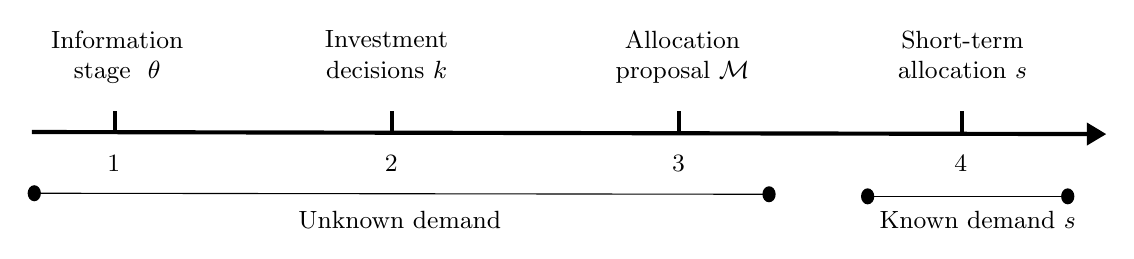
\begin{tikzpicture}[x=0.60pt,y=0.75pt,yscale=-1,xscale=1]

%Straight Lines [id:da9957648743256338] 
\draw [line width=1.5]    (20,100) -- (663,101) ;

\draw [shift={(667,101)}, rotate = 180.07] [fill={rgb, 255:red, 0; green, 0; blue, 0 }  ][line width=0.08]  [draw opacity=0] (11.61,-5.58) -- (0,0) -- (11.61,5.58) -- cycle    ;

%Straight Lines [id:da6515049842476789] 
\draw [line width=1.5,color = black]    (70,90) -- (70,100) ;
%Straight Lines [id:da5279432381947544] 
\draw [line width=1.5,color = black]   (237,90) -- (237,100) ;
%Straight Lines [id:da10457327739176892] 
\draw [line width=1.5,color = black]   (410,90) -- (410,100)  ;
%Straight Lines [id:da5055720939116881] 
\draw [line width=1.5,color = black]    (580,90) -- (580,100)   ;
%Straight Lines [id:da16737672008641513] 
\draw    (21.5,129.5) -- (464,130) ;
\draw [shift={(464,130)}, rotate = 0.06] [color={rgb, 255:red, 0; green, 0; blue, 0 }  ][fill={rgb, 255:red, 0; green, 0; blue, 0 }  ][line width=0.75]      (0, 0) circle [x radius= 3.35, y radius= 3.35]   ;
\draw [shift={(21.5,129.5)}, rotate = 0.06] [color={rgb, 255:red, 0; green, 0; blue, 0 }  ][fill={rgb, 255:red, 0; green, 0; blue, 0 }  ][line width=0.75]      (0, 0) circle [x radius= 3.35, y radius= 3.35]   ;
%Straight Lines [id:da35289334593742727] 
\draw    (523.39,131) -- (643.89,131) ;
\draw [shift={(643.89,131)}, rotate = 0] [color={rgb, 255:red, 0; green, 0; blue, 0 }  ][fill={rgb, 255:red, 0; green, 0; blue, 0 }  ][line width=0.75]      (0, 0) circle [x radius= 3.35, y radius= 3.35]   ;
\draw [shift={(523.39,131)}, rotate = 0] [color={rgb, 255:red, 0; green, 0; blue, 0 }  ][fill={rgb, 255:red, 0; green, 0; blue, 0 }  ][line width=0.75]      (0, 0) circle [x radius= 3.35, y radius= 3.35]   ;


% Text Node
\draw (30,50) node [anchor=north west][inner sep=0.75pt]  [font=\small] [align=center] {Information \\ stage  \ $\displaystyle \theta $};
% Text Node
\draw (195,50) node [anchor=north west][inner sep=0.75pt]  [font=\small] [align=center] {Investment  \\ decisions $\displaystyle k$};
% Text Node
\draw (370,50) node [anchor=north west][inner sep=0.75pt]  [font=\small] [align=center] {Allocation  \\ proposal $\displaystyle \mathcal{M}$};
% Text Node
\draw (540,50) node [anchor=north west][inner sep=0.75pt]  [font=\small] [align=center] {Short-term \\ allocation $\displaystyle s$};
% Text Node
\draw (179,137) node [anchor=north west][inner sep=0.75pt]  [font=\small] [align=center] {Unknown demand $ $};
% Text Node
\draw (529,137) node [anchor=north west][inner sep=0.75pt]  [font=\small] [align=center] {Known demand $\displaystyle s$ $ $};


\draw (64,110) node [anchor=north west][inner sep=0.75pt]  [font=\small] [align=left] {$1$};
% Text Node
\draw (231,110) node [anchor=north west][inner sep=0.75pt]  [font=\small] [align=left]  {$2$};
% Text Node
\draw (404,110) node [anchor=north west][inner sep=0.75pt]  [font=\small] [align=left]  {$3$};
% Text Node
\draw (574,110) node [anchor=north west][inner sep=0.75pt]  [font=\small] [align=center]  {$4$};

\end{tikzpicture}

\end{tcolorbox}

    %%%%%%%%%%%%%%%%%%%%    %%%%%%%%%%%%%%%%%%%%    %%%%%%%%%%%%%%%%%%%%    %%%%%%%%%%%%%%%%%%%%    %%%%%%%%%%%%%%%%%%%%    %%%%%%%%%%%%%%%%%%%%

%%%%%%%%%%%%%%%%%%%%%%%%%%%%%%%%%%%%%%%%%%%%%%%%%%%%%%%%%%%%%%%%%%%%%%%%%%%%%%%%%%%%%%%%%%%%%%%%%%%%%%%%%%%%%%%%%%%%%%%%%%%%%%%%%%%%%%%%%%%%%%%%%%%%%%%%%%%%%%%%%%%%%%%%%%%%%%%%%%%%%%%%%%%%%%%%%%%%%%%%%%%%%%%%%%%%%%%%%%%%%%%%%%%%%%%%%%%%%%%%%%%%%%%%%%%%%%%%%%%%%%%%%%%%%%%%%%%%%%%%%%%%%%%%%%%%%%%%%%%%%%%%%%%%%%%%%%%%%%%%%%%%%%%%%%%%%%%%%%%%

%%%%%%%%%%%%%%%%%%%%%%%%%%%%%%%%%%%%%%%%%%%%%%%%%%%%%%%%%%%%%%%%%%%%%%%%%%%%%%%%%%%%%%%%%%%%%%%%%%%%%%%%%%%%%%%%%%%%%%%%%%%%%%%%%%%%%%%%%%%%%%%%%%%%%%%%%%%%%%%%%%%%%%%%%%%%%%%%%%%%%%%%%%%%%%%%%%%%%%%%%%%%%%%%%%%%%%%%%%%%%%%%%%%%%%%%%%%%%%%%%%%%%%%%%%%%%%%%%%%%%%%%%%%%%%%%%%%%%%%%%%%%%%%%%%%%%%%%%%%%%%%%%%%%%%%%%%%%%%%%%%%%%%%%%%%%%%%%%%%%

\section{Complete Information}\label{chap3sec:sec3}

% In this section, we focus on the environment where the market designer determines the investment level and the wholesale market allocation.

%%%%%%%%%%%%%%%%%%%%%%%%%%%%%%%%%%%%%%%%%%%%%%%%%%%%%%%%%%%%%%%%%%%%%%%%%%%%%%%%%%%%%%%%%%%%%%%%%%%%%%%%%%%%%%%%%%%%%%%%%%%%%%%%%%%%%%%%%%%%%%%%%%%%%%%%%%%%%%%%%%%%%%%%%%%%%%%%%%%%%%%%%%%%%%%%%%%%%%%%%%%%%%%%%%%%%%%%%%%%%%%%%%%%%%%%%%%%%%%%%%%%%%%%%%%%%%%%%%%%%%%%%%%%%%%%%%%%%%%%%%%%%%%%%%%%%%%%%%%%%%%%%%%%%%%%%%%%%%%%%%%%%%%%%%%%%%%%%%%%

% \subsection{Optimal allocation proposal}

The first regime we study is the complete information case concerning consumer type. It can be understood as a nonstrategic regime with complete information in the sense that consumers reveal their type honestly. For each realization of the shock $s$, we define the allocation under complete information with $q^*_i(\theta, s)$ that maps the observed type of each consumer for each category to the quantity allocated. The monetary transfer $t^*_i(\theta,s)$ maps the observed type of each consumer to the payment made by the consumer to the market designer. This framework can be understood as the market designer offering a price/quantity allocation schedule that varies depending on the demand shock $s$ and type $\theta$. We derive the optimization problem as follows:

%%%%%%%%%%%%%%%%%%%%%%%%%%%%%%%%
\begin{align*}
\max_{\substack{ t_i(\theta,s) , \\ q_i(\theta,s) }}  \quad \quad &  CS(k) =  \sum_i  \mu_i \int_s  \int_{\theta_i} \left(U(q_i(\theta,s),\theta,s)  -  t_i(\theta,s)\right) dG_i(\theta) dF(s) \quad  \\
  \text{s.t.} \quad\quad & I(k)   \leq   \sum_i \mu_i \int_s   \int_{\theta_i}  t_i(\theta,s)    dG_i(\theta)   dF(s) ,         \tag{R}\\
    &\sum_i \mu_i \int_{\theta_i} q_i(\theta,s) dG_i(\theta) \leq k, \tag{K}
\end{align*}
%%%%%%%%%%%%%%%%%%%%%%%%%%%%%%%%

The first constraint follows the principle that the market designer should avoid any negative revenue at the optimum level of investment. It allows the rewrite of the objective function by replacing the payment part directly with the investment cost. For consistency with the rest of the analysis, we keep this constraint separated. In other words, under the supply-side assumption and given the absence of production cost, the entire income is allocated to financing the investment costs. The second constraint is the capacity constraint. We also implicitly include conditions such that $q_i$ and $t_i$ are positive and that every consumer derives a null or positive surplus when participating in the mechanism. Finally, from a timing perspective, the constraints should be considered simultaneously.\footnote {In a previous version of this paper, we develop the implications of having sequential constraints.}

We show in Proposition \ref{propch3:prop1} that under a general mechanism: $i)$, the optimal allocation is defined by a unique quantity schedule and an infinite set of monetary transfers. $ii)$ 




(1) The optimal schedule in price (unit monetary transfer) and quantity. (2) The market allocation implements the first-best schedule. Recall the market allocation is defined by a price $t_i$ linked to the allocation schedule $q_i$ such that $q_i(\theta,s) = d(t_i(\theta,s),s)$ with $d(t,\theta,s) = u^{-1}(t,\theta ,s)$. Moreover, let's define the inverse demand function: 

\begin{equation*}
    p(q,s) = \sum_i\mu_i \int_s \int_{\theta_i} u(q,\theta,s) dG_i(\theta)dF(s)
\end{equation*}

With $s_1$ as the first state of the world when the capacity is binding:

\begin{equation*}
\sum_i \mu_i \int_{\theta_i} d(0,\theta,s_1) dG_i(\theta) = 
k\end{equation*}

Then

\begin{proposition}\label{propch3:prop1}

 (1) The optimal unity monetary transfer and quantity schedule is defined for each realization of $s$ as follows:

\newlength{\tempc}
\settowidth{\tempc}{$d(p(k,s),\theta,s) \quad \quad $}

\begin{equation*}
    t^*(k,s) =
    \begin{cases}
    0 \\
    p(k,s)
   \end{cases}
\quad \text{and} \quad  
    q^*_i(k,\theta,s)  =
    \begin{cases}
    \makebox[\tempc][l]{$d(0,\theta,s)$} \quad  \quad \text{if} \quad s \in [0,s_1) \\
    \makebox[\tempc][l]{$d(p(k,s),\theta,s)$} \quad \quad \text{if} \quad s \in [s_1 , \bar{s}] 
   \end{cases}
\end{equation*}



% (2) The optimal level of investment is given by the equality between the marginal investment cost and the expected aggregate marginal utility when the capacity is binding:
% %%%%%%%
% \begin{equation*}
% k^* = \left\{ \quad k \quad | \quad r = \sum_i \mu_i \int_{s_1}^{\bar{s}}\int_{\theta_i} u(k,\theta,s) dG_i(\theta) dF(s) \right\}
% \end{equation*}

(2) If the market designer implements a market mechanism with a supply function given by the monetary transfer schedule $t^*(k,s)$ and when consumers offer truthfully their demand functions, the market outcome is the first-best allocation.

\end{proposition}

\begin{proof}
See Appendix \ref{ch3app:Ap1}
\end{proof}

Solving for the Lagrangean shows that when the capacity is not biding, the optimal allocation is characterized by an expected marginal utility null. On the other hand, when the capacity is binding, the optimal allocation should be equal to the marginal investment cost. It implies that the optimal allocation is such that the marginal utility should be equal in every state of the world. The equivalence between the first-best and market allocation can be understood by adding a new constraint to the maximization problem called $(M)$ and equal to $q_i(\theta,s) = d(t_i(\theta,s),\theta,s)$. In that case, the two maximization problems lead to the same outcomes.

The results of this proposition are at the core of how markets in the electricity system should work. Whenever the capacity is not constraining, prices equal the short-term marginal cost, i.e. the marginal production cost, which is null in this framework. When the capacity is binding, prices should be raised above the long-term marginal cost such that the expected prices during those periods equal the marginal investment cost. Given the maximization objective, the optimal transfer between consumers and the market designer for each $s$ is identical to implementing the single price given by the aggregate inverse demand function at the capacity level. 

% With the linear model, we can express the expected consumer surplus in three intermediate cases depending on the level of investment $k$ and the realization of the demand shock $s$: (i) the capacity always binds for any $s$, that is, for low values of $k$ we have $s_1=0$, (ii) the capacity never binds for any $s$, that is high values of $k$ we have $s_1 = \bar{s}$ (iii) the capacity binds for some $s$, that is for intermediate values of $k$ we have $s_1\in[0,\Bar{s}]$. For the last case, we can express, for instance, the expected consumer utility under the optimal single-price allocation as follows\footnote{In the rest of the paper, we do not always study all the possible cases depending on the value of $k$, as they do not change the theoretical results. We keep the last one as the main reference.}:

% \begin{equation*}
%     \sum_i \mu_i  \left[\int_0^{s_1}\ \underbrace{ \int_{\theta_i} U(d(0,\theta,s),\theta,s) dG_i(\theta)}_\text{off-peak utility} dF(s)        +  \int_{s_1}^{\bar{s}} \underbrace{\int_{\theta_i} U(d( p^k,\theta,s),\theta,s) dG_i(\theta)}_\text{on-peak utility}dF(s) \right]
% \end{equation*}

% $p^k = p(k,s)$ is defined for notation clarity as the aggregate demand function at the investment level $p(k,s)$.


%%%%%%%%%%%%%%%%%%%%%%%%%%%%%%%%%%%%%%%%%%%%%%%%%%%%%%%%%%%%%%%%%%%%%%%%%%%%%%%%%%%%%%%%%%%%%%%%%%%%%%%%%%%%%%%%%%%%%%%%%%%%%%%%%%%%%%%%%%%%%%%%%%%%%%%%%%%%%%%%%%%%%%%%%%%%%%%%%%%%%%%%%%%%%%%%%%%%%%%%%%%%%%%%%%%%%%%%%%%%%%%%%%%%%%%%%%%%%%%%%%%%%%%%%%%%%%%%%%%%%%%%%%%%%%%%%%%%%%%%%%%%%%%%%%%%%%%%%%%%%%%%%%%%%%%%%%%%%%%%%%%%%%%%%%%%%%%%%%%%

%%%%%%%%%%%%%%%%%%%%%%%%%%%%%%%%%%%%%%%%%%%%%%%%%%%%%%%%%%%%%%%%%%%%%%%%%%%%%%%%%%%%%%%%%%%%%%%%%%%%%%%%%%%%%%%%%%%%%%%%%%%%%%%%%%%%%%%%%%%%%%%%%%%%%%%%%%%%%%%%%%%%%%%%%%%%%%%%%%%%%%%%%%%%%%%%%%%%%%%%%%%%%%%%%%%%%%%%%%%%%%%%%%%%%%%%%%%%%%%%%%%%%%%%%%%%%%%%%%%%%%%%%%%%%%%%%%%%%%%%%%%%%%%%%%%%%%%%%%%%%%%%%%%%%%%%%%%%%%%%%%%%%%%%%%%%%%%%%%%%
\section{Incomplete Information - Fixed price}\label{chap3sec:sec4}

%% CITE HOlland and borenstein

% In this section, we use our previous results to study how the single price allocation with the spot market schedule performs in an incomplete environment. We analyze different regimes depending on (i) consumers being able to reveal their type and (ii) consumers behaving strategically. 

In this section, we study the second regime under which the market designer has to choose the best allocation,  given the following assumptions:

\begin{assumption}
(1) The consumer's type is unknown to the market designer. (2) The market designer cannot extract any information from consumers. (3) The price schedule offered by the market designers is constrained to a unique price for every state of the world. (4) Given a set of prices $t^r_i$, the market designer implements a market allocation until the capacity is not binding, and the market designer implements a rationing policy when the capacity is binding.
\end{assumption}

The first assumption implies an incomplete information framework. The second assumption means that when offering the best allocation, the market designer is not subject to incentive compatibility constraints. The third assumption provides a more realistic approach between the complete first-best allocation and the incomplete information case with a mechanism design setup described in the next section. Indeed, it approximates the actual management of essential goods such as retail electricity or public transport, where a market designer is constrained in its short-term allocation while having imperfect information on its consumers' type. To capture the effect of incomplete information, the market designer must be constrained when implementing the mechanism. It can come (i) from the quantity allocation - that is, consumers do not maximize their utility\footnote{See for instance \cite{martimort2020nonlinear} which studies the optimal monopoly nonlinear pricing in an incomplete information setting where consumers wrongly equal marginal benefit with average price. For empirical evidence, see \cite{ito2014consumers}.} - (ii) or from the proposed monetary transfer. In the last case, the price schedule is incomplete because it is not optimal for every value of $s$. It distorts the quantity consumers demand, even though it maximizes their utility.\footnote{In current practice, political and technological constraints imply that the market designer (or any retailer) can only propose a finite number of schedules. See, for instance, \cite{astier2021second} for theoretical and empirical implications for consumer surplus of allocation incompleteness.} In this paper, we take the second interpretation: We assume that the market designer can only choose a single price for every state $s$. From a policy perspective, this is similar to a market designer offering a fixed-price contract to consumers.
% \footnote{An important caveat is that when considering the case with a discrete number of consumers, a first-best allocation does not replicate the optimal allocation in incomplete information. That is, even with a complete set of prices, private information leads to inefficiencies.} 

We study two cases: (i) in Appendix \ref{AppSec:singleprice} the market designer does not discriminate between different categories, and the offered price is unique for every consumer; (ii) in this section the market designer can discriminate between different categories, and he offers a price for each category.
% \footnote{Political or technical reasons can prevent the market designer from distinguishing between different categories. It will be apparent in the section that even though the outcome of discrimination is welfare-enhancing, it is not always Pareto-improving for every category. } 
The first case allows us to focus the analysis on highlighting the trade-off the market designer faces when collecting revenue for the investment cost. In contrast, the second case highlights the distributive effect between consumers of different groups. 

This modeling approach underlines a market designer's trade-off concerning the uncertainty of the consumers' types, even without strategic inefficiencies. The core idea of the model is that, without any information, a market designer has to choose a price $t^r_i$ independent of the world's states $s$. However, one issue remains unanswered, which is how quantities are allocated within the framework. While the choice of a unique price forever consumer does not need any information concerning consumer type, the market designer still has to choose how to allocate the goods between consumers. In this section, we make the following assumption:  When the capacity is not binding, quantity is adjusted given the price price $t^r_i$. When the capacity is binding, a random allocation is implemented because of incomplete information.
% \footnote{This is not the only mechanism the market designer can implement. Indeed, we could assume a mechanism design approach where the market designer can also choose $q_i(\theta,s)$ when the capacity is not binding. In that case, the market designer produces the total quantity as in the first best and allocates it randomly to the consumers. We find that there is no clear ranking between the two mechanisms regarding consumer surplus, which depends on the model parameters. The market allocation minimizes the cross-subsidies between consumers, but when prices determine the quantity when the capacity is not binding, it induces a negative price effect. This section aims to illustrate current practice, and the two mechanisms do not fundamentally differ. Therefore, we choose to represent the market allocation approach.}
Following the framework description, we modify the actions taken by the market designer. The allocation proposal comprises (i)  choosing $t^r_i$ and (ii) defining the rationing policy $\alpha^r_i$ described below (that is, the share of capacity each consumer is receiving when capacity is binding). Below, we provide an updated figure considering the decisions the market designer has to make within this framework.

    %%%%%%%%%%%%%%%%%%%%    %%%%%%%%%%%%%%%%%%%%    %%%%%%%%%%%%%%%%%%%%    %%%%%%%%%%%%%%%%%%%%    %%%%%%%%%%%%%%%%%%%%    %%%%%%%%%%%%%%%%%%%%
\vspace{1 cm}

\tikzset{every picture/.style={line width=0.75pt}} %set default line width to 0.75pt        

\begin{tcolorbox}[colback=white]


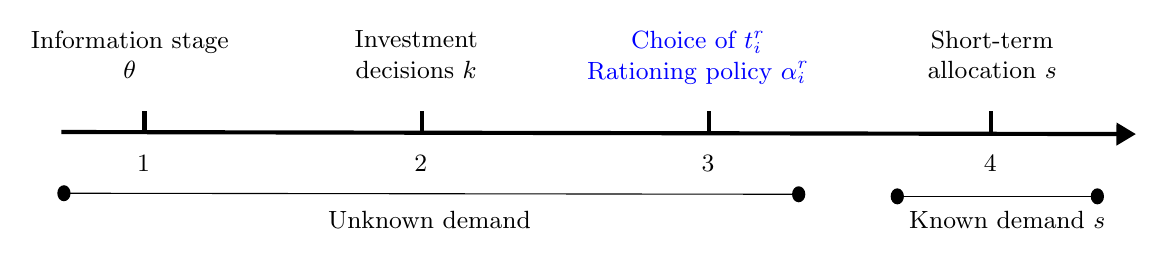
\begin{tikzpicture}[x=0.60pt,y=0.75pt,yscale=-1,xscale=1]

%Straight Lines [id:da9957648743256338] 
\draw [line width=1.5]    (20,100) -- (663,101) ;

\draw [shift={(667,101)}, rotate = 180.07] [fill={rgb, 255:red, 0; green, 0; blue, 0 }  ][line width=0.08]  [draw opacity=0] (11.61,-5.58) -- (0,0) -- (11.61,5.58) -- cycle    ;

%Straight Lines [id:da6515049842476789] 
\draw [line width=1.5,color = black]    (70,90) -- (70,100) ;
%Straight Lines [id:da5279432381947544] 
\draw [line width=1.5,color = black]   (237,90) -- (237,100) ;
%Straight Lines [id:da10457327739176892] 
\draw [line width=1.5,color = black]   (410,90) -- (410,100)  ;
%Straight Lines [id:da5055720939116881] 
\draw [line width=1.5,color = black]    (580,90) -- (580,100)   ;
%Straight Lines [id:da16737672008641513] 
\draw    (21.5,129.5) -- (464,130) ;
\draw [shift={(464,130)}, rotate = 0.06] [color={rgb, 255:red, 0; green, 0; blue, 0 }  ][fill={rgb, 255:red, 0; green, 0; blue, 0 }  ][line width=0.75]      (0, 0) circle [x radius= 3.35, y radius= 3.35]   ;
\draw [shift={(21.5,129.5)}, rotate = 0.06] [color={rgb, 255:red, 0; green, 0; blue, 0 }  ][fill={rgb, 255:red, 0; green, 0; blue, 0 }  ][line width=0.75]      (0, 0) circle [x radius= 3.35, y radius= 3.35]   ;
%Straight Lines [id:da35289334593742727] 
\draw    (523.39,131) -- (643.89,131) ;
\draw [shift={(643.89,131)}, rotate = 0] [color={rgb, 255:red, 0; green, 0; blue, 0 }  ][fill={rgb, 255:red, 0; green, 0; blue, 0 }  ][line width=0.75]      (0, 0) circle [x radius= 3.35, y radius= 3.35]   ;
\draw [shift={(523.39,131)}, rotate = 0] [color={rgb, 255:red, 0; green, 0; blue, 0 }  ][fill={rgb, 255:red, 0; green, 0; blue, 0 }  ][line width=0.75]      (0, 0) circle [x radius= 3.35, y radius= 3.35]   ;


% Text Node
\draw (0,50) node [anchor=north west][inner sep=0.75pt]  [font=\small] [align=center] {Information stage \\ $\theta$};
% Text Node
\draw (195,50) node [anchor=north west][inner sep=0.75pt]  [font=\small] [align=center] {Investment  \\ decisions $\displaystyle k$};
% Text Node
\draw (335,50) node [anchor=north west][inner sep=0.75pt]  [font=\small] [align=center] { \textcolor{blue}{Choice of $t^r_i$} \\ \textcolor{blue}{Rationing policy $\alpha_i^r$}};
% Text Node
\draw (540,50) node [anchor=north west][inner sep=0.75pt]  [font=\small] [align=center] {Short-term \\ allocation $\displaystyle s$};
% Text Node
\draw (179,137) node [anchor=north west][inner sep=0.75pt]  [font=\small] [align=center] {Unknown demand $ $};
% Text Node
\draw (529,137) node [anchor=north west][inner sep=0.75pt]  [font=\small] [align=center] {Known demand $\displaystyle s$ $ $};


\draw (64,110) node [anchor=north west][inner sep=0.75pt]  [font=\small] [align=left] {$1$};
% Text Node
\draw (231,110) node [anchor=north west][inner sep=0.75pt]  [font=\small] [align=left]  {$2$};
% Text Node
\draw (404,110) node [anchor=north west][inner sep=0.75pt]  [font=\small] [align=left]  {$3$};
% Text Node
\draw (574,110) node [anchor=north west][inner sep=0.75pt]  [font=\small] [align=center]  {$4$};

\end{tikzpicture}

\end{tcolorbox}

    %%%%%%%%%%%%%%%%%%%%    %%%%%%%%%%%%%%%%%%%%    %%%%%%%%%%%%%%%%%%%%    %%%%%%%%%%%%%%%%%%%%    %%%%%%%%%%%%%%%%%%%%    %%%%%%%%%%%%%%%%%%%%


% \subsection{Category-price policy}

We start by defining the rationing policy under this framework. This stage boils down to allocating the capacity $k$ in the first step between the two categories and the second step, randomly for each consumer within each category. We find that the market designer allocates the same expected quantity to each category under the first-best allocation (even though the within-category allocation remains inefficient). The problem is solved as follows. Let the quantity for category $i$ be $q_i$; then, when the capacity is constraining, we must have for every state of the world: $\sum_i \mu_i q_i  = k$, implying that the relation between the quantity is equal to $q_i(q_j) = \frac{k - \mu_{j}q_j}{\mu_i}$. Then, we maximize the short-term expected utility given the previous relation. Solving using the first-order condition leads to a capacity share for each consumer belonging to a group $i$ equals the allocation under the first-best allocation. 

Given this optimal rationing policy, we now define the new problem the market designer faces: 

\begin{align*}
\max_{\substack{ k  }} \max_{\substack{ t^r_i}}  \quad &  CS^r(k,t^r_1,t^r_2) =  \sum_i  \mu_i \int_s   \int_{\theta_i}( U(q^r_i(\theta,s),\theta,s)    -  t^r_i q^r_i(\theta,s) )dG_i(\theta) )\quad dF(s) \quad  \\
  \text{s.t.} \quad\quad & I(k)   \leq   \sum_i \mu_i  \int_s   \int_{\theta_i}t^r_i q^r_i(\theta,s)
     dF(s) ,         \tag{R}
\end{align*}

We drop the capacity constraint as the rationing policy defines it implicitly. To see this, we can redefine the state of the world $s^r_1$ when the capacity starts binding: 

\begin{equation*}
   \sum_i\mu_i \int_{\theta_i} d(t^r_i,\theta,s^r_1) dG_i(\theta) = k  
\end{equation*}

Then, the quantity $q^r_i(\theta,s)$ allocated in the market for each consumer of catagegory $i$ is equal to $d(t^r_i,\theta,s)$ when $s < s^r_1 $  and $ \alpha_i^r k = k + \mu_j (\theta^{av}_i - \theta^{av}_j )$ when $s \geq s^r_1$. Note that while the total quantity for each category is identical under the first-best and this framework, the total utility does differ. It implies a very similar delta in terms of utility as the equation in the Appendix \ref{AppSec:singleprice} with a single price policy. We summarize the findings in the following proposition.

% First, let's note $\mathcal{L}^r$, the Lagrangian associated with the market designer program such that 

% \begin{equation*}
%     \mathcal{L}^r(k,t^r_1,t^r_2,\gamma^r) = CS^r(k,t^r_1,t^r_2) + \gamma^r R^r(k,t^r_1,t^r_2) 
% \end{equation*}

% With $CS^r$ the aggregate expected consumer surplus defined as the sum of consumers' utility net of monetary transfers, $\gamma^r$ the lagrangian multiplier associated with the revenue constraint, and $R^r(k)$ the revenue constraint (expected revenue net of investment costs). Then, using the Envelop Theorem, we can express the derivative of an optimal price with respect to $k$ as follows:

% \begin{equation}\label{eq:diffpri}
%     \pdv{t^r_i}{k} =  \big( {CS}_{ik} +  \rho_i CS_{jk} +  (R_i - \rho_i R_j) \gamma^r_k +  (R_{ik} - \rho_i R_{jk}) \gamma^r  \big) \frac{-\mathcal{L}_{jj}}{H^r}
% \end{equation}

% \begin{equation*}
%     \gamma^r_k =   -\frac{1}{bH^r}\left(\sum_i R_i ( L_{ij} L_{jk} - L_{jj} L_{ik} ) + R_k H^r \right)
% \end{equation*}

% pdv_lamb_v1 = ...
%     - (...
%     + pdv_net_R_inc_1_k * ( L11_l * L22_l - Lij_l^2 ) ...
%     + R1_l * ( - L22_l * L1k_l + Lij_l * L2k_l) ...
%     + R2_l * ( - L11_l * L2k_l + Lij_l * L1k_l) ...
%     )/(2 * R1_l * Lij_l * R2_l - L22_l * R1_l^2 - L11_l * R2_l^2) ;
% pdv_lamb_v1_fct = matlabFunction(pdv_lamb_v1);




% pdv_lamb_v2 = simplify(...
%    ( - pdv_net_R_inc_1_k * detHess_l ...
%     + R1_l * (  L22_l * CS1k_l - Lij_l * CS2k_l ) ...
%     + R2_l * (  L11_l * CS2k_l - Lij_l * CS1k_l ) ...
%     + R1_l * lamb_1 * ( L22_l * R1k_l - Lij_l * R2k_l ) ...
%     + R2_l * lamb_1 * ( L11_l * R2k_l - Lij_l * R1k_l ) ...
%     )/detBHess_l

% \begin{equation*}
%     \pdv{t^r_i}{k} =  \big( \overbrace{{CS}_{ik} +  \rho_i CS_{jk} }^{\text{consumer surplus effect} \leq 0} \quad + \quad \overbrace{  (R_i - \rho_i R_j) \gamma^r_k +  (R_{ik} - \rho_i R_{jk}) \gamma^r  }^{\text{revenue effect }\geq 0}  \quad \big) \underbrace{{\frac{-\mathcal{L}_{jj}}{H^r}}}_{\leq 0}
% \end{equation*}


% \begin{align}\label{eq:diffpri}
%     \pdv{t^r_i}{k} =&  \overbrace{\Bigg. \frac{-\mathcal{L}_{jj}}{H^r} \Bigg. }^{\leq 0} \overbrace{\Bigg( CS_{ik} +  \rho_i CS_{jk} +   (R_i - \rho_i R_j) \sum_i( CS_{ik} -\rho_i  CS_{jk} )\frac{ {  R_i } }{L_{jj} 
%  bH^r}}^{\text{effect of $k$ on CS with holding R fixed}}  \\ 
%    & \quad + \underbrace{  \gamma^r \bigg (R_{ik} - \rho_i R_{jk} + (R_i - \rho_i R_j)\sum_i(   R_{ik} - \rho_i R_{jk} ) \frac{ R_i  }{L_{jj} bH^r} \bigg)  -  R_k\frac{{ H^r} }{bH^r}   \Bigg) }_{\text{effect of $k$ on $R$}}
% \end{align}

% \begin{equation*}
%     \pdv{t^r_i}{k} =  \big( \Big. \overbrace{{CS}_{ik} + R_i \gamma^r_k + R_{ik}\gamma^r  \Big.  }^{\text{effect of $t^r_i$}} - \rho_i(  \overbrace{ \Big.{CS}_{jk}  + R_j  \gamma^r_k +  R_{ik} \gamma^r  \Big. }^{\text{effect of $p_j^r$}} ) \big) \underbrace{\Big.{\frac{-\mathcal{L}_{jj}}{H^r}}\Big.}_{\leq 0}
% \end{equation*}

% pdv_lamb_v1 = simplify(...
%     - (...
%     + pdv_net_R_inc_1_k * ( L11_l * L22_l - Lij_l^2 )..
%     + R1_l * ( - L22_l * L1k_l + Lij_l * L2k_l)..
%     + R2_l * ( - L11_l * L2k_l + Lij_l * L1k_l)..
%     )/detBHess_l);

% \begin{equation*}
%     \gamma^r_k =\frac{ \sum_i  R_i (L_{jj} L_{ik} - L_{ij} L_{jk}) - R_k H^r }{bH^r}
% \end{equation*}


% pdv_lamb_v2 = simplify(...
%    ( - pdv_net_R_inc_1_k * detHess_l...
%     + R1_l * (  L22_l * CS1k_l - CSij_l * CS2k_l - lamb_1 * Rij_l * CS2k_l )...
%     + R2_l * (  L11_l * CS2k_l - CSij_l * CS1k_l - lamb_1 * Rij_l * CS1k_l )...
%     + R1_l * lamb_1 * ( L22_l * R1k_l - Lij_l * R2k_l )...
%     + R2_l * lamb_1 * ( L11_l * R2k_l - Lij_l * R1k_l )...
%     )/detBHess_l);
% pdv_lamb_v2_fct = matlabFunction(pdv_lamb_v2);


% \begin{equation*}
%     \gamma^r_k =\frac{ \overbrace{\sum_i  R_i (  L_{jj} CS_{ik} - L_{ij} CS_{jk} )}^{\text{CS effect}} + \overbrace{\sum_i \gamma^r R_i (  L_{jj} R_{ik} - L_{ij} R_{jk} ) - R_k H^r}^{\text{Revenue effect}} }{bH^r}
% \end{equation*}


% With $\rho_i = \frac{L_{ij}}{L_{jj}}$. $H^r = \mathcal{L}_{11}\mathcal{L}_{22} - \mathcal{L}_{12}\mathcal{L}_{21}
% $ being the determinant of the Hessian matrix of the Lagrangian. $bH^r = \mathcal{L}_{ij} R_i R_j - \mathcal{L}_{jj} R_i^2 - \mathcal{L}_{ii} R_j^2 + \mathcal{L}_{ji} R_i R_j$ being the determinant of the bordered Hessian matrix of the lagrangian. Each variable's index is associated with the corresponding derivative. For instance, $CS_{ik}$ reads as the cross derivative between the price of category $i$ with respect to the investment level. It measures the (marginal) change of the marginal effect of price $ t^r_i$ on the consumer surplus. 


\begin{proposition}\label{propch3:prop4}
    Suppose that category 1 consumers are of higher types than category 2 consumers and that the investment cost is not too high then: (1) $t^r_1(k)$ is increasing with $k$; (2) $t^r_2(k)$ is first decreasing, then increasing with $k$.
\end{proposition}

\begin{proof}
In Appendix \ref{ch3app:Ap6}, we provide the formal proof and the condition under which the results hold. It relies on two Lemmas that ensure that a minimum exists. We also provide a more technical discussion on the rationales for this proposition. 
\end{proof}

Figure \ref{fig:optpolicypr1} illustrates the results. The red curve shows $t^r_1(k)$, the blue curve shows $t^r_2(k)$, and the black dashed curve shows the optimal single price $t^r(k)$ found in Appendix \ref{AppSec:singleprice}. Following the proposition, we observe that the blue curves corresponding to the group with a lower expected demand exhibit a non-monotonic relationship with the level of investment such that it decreases for low values of $k$ and then increases again following a similar behavior to the optimal price for the higher category of consumers represented in the red curve.


\begin{figure}
    \centering
    \includegraphics[scale = 1.2]{1_figures/short/optpolicypr1_pttv2.png}
    \caption{Optimal prices under the category-price policy with respect to the investment}
    \label{fig:optpolicypr1}
\end{figure}

The proof of such behavior of the optimal prices can be understood by distinguishing the first-order and the second-order effects of prices and level of investment on (a) the aggregate consumer surplus and (b) the revenue constraint. The non-monotonicities of prices are the result of a \textbf{consumer surplus effect} dominating first a \textbf{revenue effect} for low values of $k$, then the revenue effect dominating the consumer effect for higher values of $k$.


% We summarize this tension between consumer and revenue effects in the following equation, which is a more detailed expression of Equation \ref{eq:diffpri}.

% \begin{align*}
%     \pdv{t^r_i}{k} =&  \overbrace{\Bigg. \frac{-\mathcal{L}_{jj}}{H^r} \Bigg. }^{\leq 0} \Bigg( \overbrace{CS_{ik} +  \rho_i CS_{jk} +   (R_i - \rho_i R_j) \sum_i( CS_{ik} -\rho_i  CS_{jk} )\frac{ {  R_i } }{L_{jj} 
%  bH^r}}^{\text{effect of $k$ on CS with holding R fixed}}  \\ 
%    & \quad + \underbrace{  \gamma^r \bigg (R_{ik} - \rho_i R_{jk} + (R_i - \rho_i R_j)\sum_i(   R_{ik} - \rho_i R_{jk} ) \frac{ R_i  }{L_{jj} bH^r} \bigg)  -  R_k\frac{{ H^r} }{bH^r} }_{\text{effect of $k$ on $R$}}  \Bigg) 
% \end{align*}

As shown in Appendix \ref{AppSec:singleprice}, this framework implies that a change of $k$ does affect both revenue and the consumer surplus, which is captured via the direct effect on prices needed for financing this investment and the change of occurrences between off-peak and on-peak periods. First, the level of investment induces a positive first derivative of the consumer surplus and a negative second derivative. That is, increasing $k$ always increases the surplus, but for a higher level of investment, the positive impact is relatively smaller. On the other hand, an analysis of how the revenue constraint behaves shows a convex effect with respect to $k$. It implies that an increase of $k$ leads to the revenue constraint shifting at an increasing rate.\footnote{The pure revenue effect of increasing prices is found in Appendix \ref{AppSec:singleprice}. The intuition is that when $k$ increases, the marginal gain from an increase of capacity during on-peak periods is offset by the increase in investment costs and by the decrease of on-peak periods. In the Appendix, we formally demonstrate that $t^r$ is convex with respect to $k$.} The switch between the decreasing and increasing parts is associated with the consumer surplus effect dominating the revenue effect first. As $k$ increases, the respective concavity and convexity of the functions lead to the revenue effect dominating the surplus effect.

The increasing prices on the right part of Figure \ref{fig:optpolicypr1} can be understood through the results of Proposition \ref{propch3:prop3}. The ranking between the category prices stems from the preference for discriminating bigger consumers. Increasing $t^r_1$ generates more revenue as they consume, on average, more. 

Let us turn towards the left part of Figure \ref{fig:optpolicypr1}. We show why the asymmetry between the two consumers decreases for a higher value of $k$. Indeed, we find that this is not fully due to the revenue effect. For the sake of clarity, let's assume the revenue does not depend on $k$. We study the impact of $k$ on the indifference curve of the market planner with respect to the prices $t^r_1$ and $t^r_2$. We define the marginal rate of substitution between the two prices:


\begin{align*}
    MRS_{i \rightarrow j}(k) = \frac{CS^r_i}{CS^r_j}
\end{align*}

It implies that the MRS changes with respect to $k$ as follows:

\begin{align*}
    \pdv{MRS_{i \rightarrow j}}{k} = \frac{CS^r_{ik}CS^r_j - CS^r_{jk}CS^r_i}{{CS^r_j}^2}
\end{align*}

Therefore, the decreasing right part of prices can be explained by having $\pdv{MRS_{i \rightarrow j}}{k} < 0$. As the level of investment increases, and to keep the same level of consumer surplus, a decrease in $t^r_i$ should lead to a relatively smaller increase of $t^r_j$. The economic interpretation of the effect of $k$ can be understood as follows. As $k$ increases, it negatively impacts the (negative) marginal effect of prices on consumer surplus. Because consumers from the bigger category have a higher marginal consumer surplus with respect to price, the negative marginal effect of prices of $k$ is bigger than for the consumers from the smaller category. In other words, as $k$ increases, $CS_i$ decreases faster than $CS_j$, which implies a negative effect on the MRS. This can be explained by the fact that as $k$ increases, it lowers the occurrences of on-peak periods, which makes consumers more exposed to the negative price effect on the quantity during off-peak periods. This, in turn, incites the market designer to have lower prices, which is attained by lowering discrimination.

% We illustrate this intuition in Figure \ref{fig:illustTMS}. We represent a fixed revenue constraint as well as two indifference curves with respect to $t^r_1$ and $t^r_2$ for two values of $k$.  As $k$ increases, we show that the indifference curves tend to decrease in the sense that their marginal rate of substitution decreases with $k$. It is this shift in the shape of the consumer surplus that implies a decrease in the optimal price, meaning that the gain in lower prices is higher than the gain from discrimination.  

% \begin{figure}
%     \centering
%     \includegraphics{1_figures/short/illustTMS.png}
%     \caption{Illustration of the decreasing part of $t^r_2$ with respect to $k$}
%     \label{fig:illustTMS}
% \end{figure}



% We conclude this section by analyzing the implication of the optimal policy when choosing the level of investment to maximize the consumer surplus. We define the first-order conditions using the Envelop Theorem for constrained optimization. That is, it is sufficient to derive the derivative of the Lagrangian with respect to $k$: $\pdv{\mathcal{L}^r }{k} = \pdv{CS^r}{k} + \gamma^r \pdv{R^r}{k}$. We start with the individual consumer surplus\footnote{We use the individual surplus for clarity. The aggregate surplus exhibits similar behavior.}:

% \begin{align*}
%          &  \overbrace{   \int_{\alpha_i^r k}^{d(t^r_i,\theta,s^r_1)} u(q,\theta,s^r_1) dq }^{\text{$\Delta$ in quantity btw. off-peak and on-peak}}+ \overbrace{\int_{s^r_1}^{\bar{s}} ( u( \alpha_i^r k, \theta,s) - t^r_i) dF(s)}^{\text{$+$ in on-peak CS}} 
% \end{align*}

% The second term is similar to the complete information benchmark. It represents the gain in consumer surplus during on-peak as capacity expands. Note that the gain in surplus does not depend on the price as the quantity is randomly assigned to each consumer in each category due to imperfect information. The first term stands for the change at the margin of quantities for each consumer. Under complete information, the quantities allocation is continuous in $s$. However, due to incomplete knowledge, the market designer creates a discontinuity in the allocation when capacity starts binding, which implies that the value at $s^r_1$ does not cancel out. For the revenue, the derivative can be expressed as follows: 

% \begin{align*}
%          &  \overbrace{ \Bigg. \sum_i\mu_i \int_{\theta_i} t^r_i \bigg( d(t^r_i,\theta,s^r_1) - \alpha_i^r k \bigg) dG_i(\theta)  \Bigg.}^{\text{$\Delta$ in quantity btw. off-peak and on-peak}}+ \overbrace{\int_{s^r_1}^{\bar{s}}  \Bigg. \sum_i\mu_i t^r_i dF(s)\Bigg. }^{\text{$+$ in on-peak rev.}}   - r
% \end{align*}

% The first term is similar and originates from discontinuity. The second term comes from the increase in available quantity during on-peak. As expected, and similarly to the first-best investment level, the sign of the first-order condition is ambiguous as it has positive and negative effects of an increase in $k$. For instance, it raises investment costs, but it also raises available revenue. Calculations show that a level of investment exists that maximizes the expected aggregate consumer surplus, as the consumer surplus and the revenue are concave in $k$. 




\section{Incomplete Information - Mechanism Design}\label{chap3sec:sec5}


\subsection{Optimal allocation}

We extend the previous framework by allowing the market designer to choose an allocation mechanism such that (i) consumers behave truthfully and (ii) the market designer is not constrained in its choice of prices given the realization of $s$. The two assumptions combined allow him to bypass the spot market allocation because truthful behavior implies that he can also set quantities for each consumer. In other words, the market designer can now offer a complete set of prices and quantities such that the schedule depends on each consumer, for every state of the world $s$, and every type $\theta$. The following figure summarizes the new action set for the market designer. As we will show, the incentive compatibility constraint pins down the optimal monetary transfer $t^m_i$, leaving the market designer only with the quantity choice.



    %%%%%%%%%%%%%%%%%%%%    %%%%%%%%%%%%%%%%%%%%    %%%%%%%%%%%%%%%%%%%%    %%%%%%%%%%%%%%%%%%%%    %%%%%%%%%%%%%%%%%%%%    %%%%%%%%%%%%%%%%%%%%
\vspace{1 cm}

\tikzset{every picture/.style={line width=0.75pt}} %set default line width to 0.75pt        

\begin{tcolorbox}[colback=white]


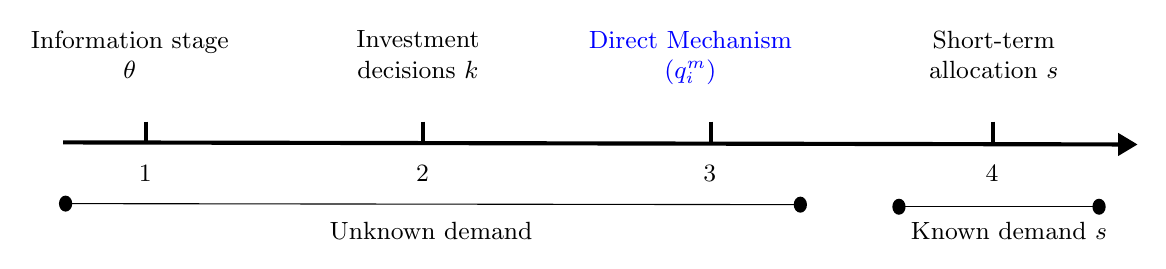
\begin{tikzpicture}[x=0.60pt,y=0.75pt,yscale=-1,xscale=1]

%Straight Lines [id:da9957648743256338] 
\draw [line width=1.5]    (20,100) -- (663,101) ;

\draw [shift={(667,101)}, rotate = 180.07] [fill={rgb, 255:red, 0; green, 0; blue, 0 }  ][line width=0.08]  [draw opacity=0] (11.61,-5.58) -- (0,0) -- (11.61,5.58) -- cycle    ;

%Straight Lines [id:da6515049842476789] 
\draw [line width=1.5,color = black]    (70,90) -- (70,100) ;
%Straight Lines [id:da5279432381947544] 
\draw [line width=1.5,color = black]   (237,90) -- (237,100) ;
%Straight Lines [id:da10457327739176892] 
\draw [line width=1.5,color = black]   (410,90) -- (410,100)  ;
%Straight Lines [id:da5055720939116881] 
\draw [line width=1.5,color = black]    (580,90) -- (580,100)   ;
%Straight Lines [id:da16737672008641513] 
\draw    (21.5,129.5) -- (464,130) ;
\draw [shift={(464,130)}, rotate = 0.06] [color={rgb, 255:red, 0; green, 0; blue, 0 }  ][fill={rgb, 255:red, 0; green, 0; blue, 0 }  ][line width=0.75]      (0, 0) circle [x radius= 3.35, y radius= 3.35]   ;
\draw [shift={(21.5,129.5)}, rotate = 0.06] [color={rgb, 255:red, 0; green, 0; blue, 0 }  ][fill={rgb, 255:red, 0; green, 0; blue, 0 }  ][line width=0.75]      (0, 0) circle [x radius= 3.35, y radius= 3.35]   ;
%Straight Lines [id:da35289334593742727] 
\draw    (523.39,131) -- (643.89,131) ;
\draw [shift={(643.89,131)}, rotate = 0] [color={rgb, 255:red, 0; green, 0; blue, 0 }  ][fill={rgb, 255:red, 0; green, 0; blue, 0 }  ][line width=0.75]      (0, 0) circle [x radius= 3.35, y radius= 3.35]   ;
\draw [shift={(523.39,131)}, rotate = 0] [color={rgb, 255:red, 0; green, 0; blue, 0 }  ][fill={rgb, 255:red, 0; green, 0; blue, 0 }  ][line width=0.75]      (0, 0) circle [x radius= 3.35, y radius= 3.35]   ;


% Text Node
\draw (-1,45) node [anchor=north west][inner sep=0.75pt]  [font=\small] [align=center] {Information stage \\ $\theta$};
% Text Node
\draw (195,45) node [anchor=north west][inner sep=0.75pt]  [font=\small] [align=center] {Investment  \\ decisions $\displaystyle k$};
% Text Node
\draw (335,45) node [anchor=north west][inner sep=0.75pt]  [font=\small] [align=center]{ \textcolor{blue}{Direct Mechanism} \\  \textcolor{blue}{$(q_i^m)$}};
% Text Node
\draw (540,45) node [anchor=north west][inner sep=0.75pt]  [font=\small] [align=center] {Short-term \\ allocation $\displaystyle s$};
% Text Node
\draw (179,137) node [anchor=north west][inner sep=0.75pt]  [font=\small] [align=center] {Unknown demand $ $};
% Text Node
\draw (529,137) node [anchor=north west][inner sep=0.75pt]  [font=\small] [align=center] {Known demand $\displaystyle s$ $ $};


\draw (64,110) node [anchor=north west][inner sep=0.75pt]  [font=\small] [align=left] {$1$};
% Text Node
\draw (231,110) node [anchor=north west][inner sep=0.75pt]  [font=\small] [align=left]  {$2$};
% Text Node
\draw (404,110) node [anchor=north west][inner sep=0.75pt]  [font=\small] [align=left]  {$3$};
% Text Node
\draw (574,110) node [anchor=north west][inner sep=0.75pt]  [font=\small] [align=center]  {$4$};

\end{tikzpicture}

\end{tcolorbox}

    %%%%%%%%%%%%%%%%%%%%    %%%%%%%%%%%%%%%%%%%%    %%%%%%%%%%%%%%%%%%%%    %%%%%%%%%%%%%%%%%%%%    %%%%%%%%%%%%%%%%%%%%    %%%%%%%%%%%%%%%%%%%%


To induce true reporting from consumers,  the market designer needs to require the following:

\begin{equation*}\label{eq:IC1}
    \theta = \arg \max_{\hat{\theta} } \int_ s(U(q_i(\hat{\theta},s),\theta,s)  - t_i(\hat{\theta},s) q_i(\hat{\theta},s))   dF(s) \tag{IR}
\end{equation*}

While the participation of every consumer implies that:

\begin{equation*}\label{eq:IR1}
    0  \leq   \int_s ( U(q_i(\theta,s),\theta,s)    -  t_i(\theta,s) q_i(\theta,s) )  dF(s) \tag{IC}
\end{equation*}

In that case, the mechanism design problem faced by the market designer is given by:

%%%%%%%%%%%%%%%%%%%%%%%%%%%%%%%%
\begin{align*} \label{eq:pbMD}
\max_{\substack{ k  }} \max_{\substack{ t_i(\theta,s) , \\ q_i(\theta,s) }}  \quad \quad &  CS(k) =  \sum_i  \mu_i \int_s     \int_{\theta_i} (U(q_i(\theta,s),\theta,s)    -  t_i(\theta,s) q_i(\theta,s)) dG_i(\theta) dF(s) \quad  \\
  \text{s.t.} \quad\quad & I(k) \leq \sum_i \mu_i \int_s  \int_{\theta_i}( t_i(\theta,s) q_i(\theta,s)) dG_i(\theta) dF(s) ,         \tag{R}\\
    & \sum_i \mu_i \int_s \int_{\theta_i} q_i(\theta,s) dG_i(\theta) dF(s) \leq k, \tag{K} \\
    & 0  \leq   \int_s ( U(q_i(\theta,s),\theta,s)    -  t_i(\theta,s)) q_i(\theta,s)   dF(s), \tag{IR} \\
   & \theta = \arg \max_{\hat{\theta} } \int_ s(U(q_i(\hat{\theta},s),\theta,s)  - t_i(\hat{\theta},s) q_i(\hat{\theta},s) )  dF(s) , \tag{IC}
\end{align*}
%%%%%%%%%%%%%%%%%%%%%%%%%%%%%%%%

We start describing the optimal allocation schedule given the new constraints and for a given level of investment $k$. Using the method developed in \cite{GUESNERIE1984329} and \cite{spulber1992capacity}, we characterize the monetary transfer $t_i(\theta,s)$ in terms of quantity $q_i(\theta,s)$. As the problem is well-defined, the incentive compatibility constraint is satisfied as soon as the optimal allocation $q_i(\theta,s)$ increases with respect to the type $\theta$. The payoff equivalence implies the following relation between optimal transfer and quantity allocated to a consumer of type $\theta$, from category $i$ and given a realization of $s$:

\begin{equation*}\label{eq:pequiv}
    t_i(\theta,s)q_i(\theta,s) = U(q_i(\theta,s),\theta,s) - \int_{\Bar{\theta}}^{\theta} q_i(\hat{\theta},s) d \hat{\theta} + Cst 
\end{equation*}

Where $Cst$ is an arbitrary constant. The payoff equivalence uses the canonical approach of the Envelope Theorem (see \cite{milgrom2002envelope}). Next, we use the approach from \cite{spulber1992capacity} to characterize a feasibility constraint that associates the revenue and individual rationality constraints. The core idea is that if one of the constraints is satisfied but not the other, a feasible lump-sum transfer from the non-binding constraint could exist that allows for relaxing the binding constraints. To say it differently, when there is, for instance, some excess revenue but the individual rationality is constraining, it is possible to transfer a lump-sum positive amount of money to the lowest types of consumers, which allows for less constraint optimal allocation. We describe in the following equation the corresponding new constraint, noted $R-IR$:

\begin{equation}\label{eq:RIRconstr}
        \sum_i \mu_i \int_s \int_\theta (U(q_i(\theta,s),\theta,s)  -\Gamma_i(\theta) \int_s q_i(\theta,s) dF(s) )dG_i(\theta) dF(s) - I(k) \geq 0 , \tag{R-IR}
\end{equation}

With $\Gamma_i(\theta) = \frac{1 - G_i(\theta)}{g_i(\theta)}$ the inverse hazard rate. Under the uniform distribution assumption considering the distribution of $\theta$, the inverse hazard rate is decreasing with $\theta$. We then solve for the Lagrangian. The following lemma shows the first-order condition to find the optimal allocation $q^m_i(\theta,s)$.

\begin{lemma}\label{lemch3:lem2}
    Given IC and IR constraints, the optimal allocation $q_{i,l}^m(\theta,s)$ for a consumer of type $\theta$ from category $i$ and for a given realization of $s$  satisfies the following condition.
\begin{equation*}
        u(q^m_{i,l},\theta,s)(1+\zeta) - \zeta \Gamma_i(\theta) - \varepsilon =0
\end{equation*}

With $\zeta$ and $\varepsilon$, the Lagrangian multipliers for, respectively, the $R-IR$ condition and the capacity constraint. We denote $l = \{1,2,3,4\}$ the index variable such that when $l = \{3,4\}$ implies that $R-IR$ is binding while $l = \{1,2\}$ means it does not, and $l = \{2,4\}$ implies that the capacity is binding while $ l = \{1,3\}$ means it does not.

\end{lemma}

\begin{proof}
See Appendix \ref{ch3app:Ap7}
\end{proof}

% Given the lemma, we can prove that the optimal allocation increases with the type. For instance, the following equation shows the derivative of the optimal allocation when both capacity and the $R-IR$ constraint are binding. 

% \begin{align*}
%     \/\pdv{q^m_{i,4}}{\theta}= \left(\frac{1}{2}-  {\pdv{u}{\theta} } \right)\left[1 - \frac{\zeta }{1 + \zeta }{\Gamma'_i(\theta)} \right] /{\pdv{u}{q}}
% \end{align*}

% Following the model specification, $\pdv{u}{\theta} = 1$ and $\pdv{u}{q}<0$, the assumption concerning $\Gamma'_i(\theta) < 0$ implies that $\pdv{q^m_{i,4}}{\theta}>0$. 

Lemma \ref{lemch3:lem2} provides four solutions to the problem faced by the market designer depending on which constraints are binding or not. We can regroup them in pairs such that $\{q^m_{i,1}(\theta,s),q^m_{i,2}(\theta,s)\}$ is the set of quantities when the optimal allocation is not constraint by $R-IR$. That is, the revenue generated by the mechanism is sufficient to cover the fixed costs and provide enough incentive for every consumer to consume electricity. On the other hand, $\{q^m_{i,3}(\theta,s),q^m_{i,4}(\theta,s)\}$ is the set of quantities such that the constraint is binding, implying that the optimal allocation needs to be distorted to cover both fixed costs and participation. Finally, note that the optimal allocation under the mechanism design approach when the $R-IR$ constraint is not binding is identical to the first-best allocation. Namely, when $\zeta = 0$, the condition in Lemma \ref{lemch3:lem2} is identical to the conditions described in the complete information section. Moreover, it can also be shown that the spot market schedule in prices and quantities is also incentive-compatible \citep{spulber1992capacity}. Therefore, we focus the rest of the analysis on the allocations $\{q^m_{i,3}(\theta,s),q^m_{i,4}(\theta,s)\}$.

\subsection{Optimal allocation and investment level}

We next analyze the threshold between the two sets of quantities. That is, we describe under which value of $k$ the market designer faces a binding $R-IR$. We summarize the findings in the following proposition.

\begin{proposition}\label{propch3:prop5}
    A unique value of $k$ exists such that the $R-IR$ is null. Moreover, for any value of $k$ below this threshold, the constraint $R-IR$ is not binding, while any value above the constraint is binding.
\end{proposition}

\begin{proof}
See Appendix \ref{ch3app:Ap8}
\end{proof}

Proposition \ref{propch3:prop5} shows that it is possible to cover both fixed costs and participation constraints without distorting the allocation only when the level of investment is low. The intuition for this result can be understood as follows. First, we denote the marginal virtual utility: $J_i(q,\theta,s) = u(q^m_{i,k}(\theta,s),\theta,s) - \Gamma_i(\theta)$, which is the marginal utility derived from the optimal allocation net of the information rent. Under the framework, it can be interpreted as the feasible gain in utility from the allocation after having remunerated the consumers to behave truthfully. Then, we can express the derivative of the $R-IR$ constraint for the first set of optimal quantities.

\begin{equation*}
   \overbrace{ \sum_i \mu_i \int_{s_1^r}^{\bar{s}} \int_{\theta_i} \quad J_i(q^m_{i,2},\theta,s)  \pdv{q^m_{i,2}}{k} \quad dG_i(\theta) dF(s)}^{\text{aggregate expected marginal virtual revenue}} \quad - \quad  r
\end{equation*} 

In other terms, the constraint starts binding when the aggregated marginal virtual revenue from the mechanism during the on-peak period equals the marginal investment. Note that both the marginal virtual utility and the derivative of the quantity are, in that case, positive. Under the framework, $\pdv{q_{1,2}^m}{k}$ is equal to 1, so to ensure that $\sum_i \mu_i \pdv{q_{1,2}^m}{k} = 1$. Therefore, an increase of $k$ generates an ambiguous effect on the constraint: (i) it increases the virtual surplus during on-peak periods, and (ii) it increases the investment costs. However, the expected surplus from consumers is concave. Indeed, note that the derivative of the marginal virtual utility with respect to $k$ is equal to $\pdv{J_i}{k} =- \pdv{q^m_{i,k}}{k}$, meaning that if an increase of the investment increases the optimal quantity, then it decreases the possible marginal utility net of information rent. This effect also accumulates with the change in occurrence between off-peak and on-peak. As $k$ increases, the capacity binds less in expectation, implying a decrease in the positive first part of the expression above. This second-order effect, combined with the increase in investment costs, implies that the constraint crosses binds only once. 

\begin{figure}
    \centering
    \includegraphics[scale = 1.2]{1_figures/short/EV_ptt.png}
    \caption{$R-IR$ constraints and its component with respect to the investment level.}
    \label{fig:EV}
\end{figure}

We illustrate the findings in Figure \ref{fig:EV}. We plot the $R-IR$ constraint under the optimal allocation set $\{q^m_{i,1},q^m_{i,2}\}$ for different values of $k$. The black curve shows the constraint. We decompose it with the blue curve only representing the aggregate expected consumer virtual utility and the red curve representing the investment costs. As previously described, the blue curve is concave in $k$ with an increasing value and then a decreasing part. Note that for sufficiently high values of $k$, the utility function is even independent of $k$ because, in expectation, the capacity is never binding.  When adding the increasing investment costs, the difference between the two has to exhibit, at one point, a decreasing behavior. Finally, we have represented the threshold value with the vertical dashed line. For lower values of $k$, the $R-IR$ constraint is positive, meaning that fixed costs and the information constraint are not binding. Above this value, the value is negative, so the market designer needs to distort the allocation so that $R-IR =0$. We now describe how the optimal allocation depends on the investment level when the $R-IR$ binds. We summarize the main findings in the following proposition. We define the term $\mathbb{A}(k)$ in the Appendix \ref{ch3app:Ap9} such that we have $\pdv{\zeta}{k} = \mathbb{A}(k)(1+\zeta(k))$. It is independent of the states of the world and the consumer types. It represents the direct marginal effects of an additional level of investment (higher investment costs and more on-peak quantities) weighted by the marginal aggregate indirect effects (due to the change in off-peak and on-peak quantities at the optimum). Then:

\begin{proposition}\label{propch3:prop6}

The investment level directly affects the optimal allocation:

\begin{itemize}[leftmargin=+0.7cm]
    \item  (Optimal off-peak) $\quad q_{i,3}^m(\theta,s)$ is always decreasing with $k$ for every values of $k$ and for every type.

\vspace{0.25 cm}

\item (Optimal on-peak) $\quad $ for a consumer belonging to category $i$ and of type $\theta$, if:

    \vspace{0.25 cm}
    
    \begin{itemize}[label=$\ast$]
        \item \( \displaystyle J_i(q_{i,4}^m,\theta,s) > \mathbb{E}J_{4} - \frac{1} {\mathbb{A}}\quad \quad 
        \) then \( q_{i,4}^m(\theta,s) \) is always increasing with $k$.

\vspace{0.25 cm}
        
        \item \( \displaystyle J_i(q_{i,4}^m,\theta,s) < \mathbb{E}J_{4} - \frac{1} {\mathbb{A}}\quad \quad   \) then \( q_{i,4}^m(\theta,s) \) is always decreasing with $k$.
    \end{itemize}



    \end{itemize}

    
\end{proposition}

\begin{proof}
See Appendix  \ref{ch3app:Ap9}.
\end{proof}

The proposition states that for a higher level of investment, every consumer should receive less electricity during off-peak periods. During on-peak, the change of quantity depends on the types. For lower types of both categories, consumers should also receive less electricity. On the other hand, higher types always receive more electricity as capacity expands. When the capacity is not binding, the effect on the quantity is captured in the equation below:

\begin{equation*}
    \pdv{q^m_{i,3}}{k} = J_i(q^m_{i,3},\theta,s) \mathbb{A}(k)
\end{equation*}

Under the framework, we find that $\mathbb{A}(k)>0$. The derivative originates from the first-order condition from Lemma \ref{lemch3:lem2}: the marginal virtual utility at the optimal allocation during off-peak is always negative. Under the framework, and similarly to the previous sections, we know that the revenue constraint behaves convexly with respect to $k$: a higher capacity level implies a higher need for revenue. Thus it implies that  $\pdv{\zeta}{k} > 0$. The two observations lead to a negative derivative. The economic intuitions can be understood as follows: as $k$ expands, this does not directly generate any additional quantity for consumers during off-peak, as, by definition, the capacity is not binding. On the other hand, the need for revenue is increasing. Combining the absent surplus effect and the negative revenue effect implies that the optimal quantities for all consumers are decreasing. For the on-peak allocation, the initial derivative is expressed as follows: 

\begin{equation*}
    \pdv{q^m_{i,4}}{k} = \left[ J_i(q^m_{i,4},\theta,s) \pdv{\zeta}{k} - \pdv{\varepsilon}{k} \right]\frac{1}{1+\zeta} 
\end{equation*}

As quantity expands, the willingness to pay for less binding constraint decreases, implying that $\pdv{\varepsilon}{k}<0$. Therefore, the sign of the derivative is ambiguous and notably depends on the sign of $J_i(q^m_{i,4},\theta,s)$. Contrary to the off-peak allocation, the initial first-order condition when $\varepsilon > 0$ does not allow a clear-cut answer for the sign of the virtual marginal utility. Using the constraint from the market design problem, we can express the derivative of the Lagrange multiplier $\varepsilon$ associated with the capacity constraint as a function of the derivative of $\zeta$ with respect to $k$. Namely, after simplification, we find that the derivative of the optimal quantity can be expressed as follows:

\begin{equation}\label{eq:q4md}
    \pdv{q^m_{i,4}}{k} = \left[ J_i(q^m_{i,4},\theta,s)  - \mathbb{E}J_{4}  \right] \mathbb{A}(k) + 1 
\end{equation}

With 

\begin{equation*}
    \mathbb{E}J_{4} = \sum_i \mu_i \int_{\theta_i} J_i(q^m_{i,4},\theta,s) dG_i(\theta)
\end{equation*}

Being the aggregate marginal virtual utility over every consumer and across all groups. The equation states a sufficient condition for having a positive derivative for a given consumer: If his virtual marginal utility is not too low than the aggregate marginal virtual utility, then its allocation is increasing with $k$. This condition captures the fundamental trade-off that the market designer faces when there is an information constraint. First, note the value 1 on the right part of the equation. It describes the positive effect of increasing $k$ for consumers when the capacity is binding, which always implies higher utility. On the other hand, the left part can be negative if the marginal virtual utility is not sufficiently close to the aggregate expression. We find that this is due to the existence of the cost associated with incomplete information. 

% \noindent \textbf{Illustrative Example} When expressing the marginal utility with respect to the optimal allocation, we find the following difference assuming two consumers of the same category, with one having type $\theta^1$ and the other having $\theta^2$. 

% \begin{equation*}
%     u(q^m_{i,4}(\theta^1,s),\theta^1,s) - u(q^m_{i,4}(\theta^2,s),\theta^2,s) = (\theta^2 - \theta^1)\frac{\zeta(k)}{1+\zeta(k)}
% \end{equation*}

% That is, smaller consumers imply smaller marginal utility at the optimal allocation. We turn now to the difference in terms of information rent: 

% \begin{equation*}
%     \Gamma_i(\theta^1) - \Gamma_i(\theta^2)  = \theta^2 - \theta^1
% \end{equation*}

% The information rent is higher with smaller consumers. The two combines leads to :

% \begin{equation*}
%     J_i(q^m_{i,4},\theta,s)(q^m_{i,4}(\theta^1,s),\theta^1,s) - J_i(q^m_{i,4},\theta,s)(q^m_{i,4}(\theta^2,s),\theta^2,s)  = (\theta^1 - \theta^2)\frac{1}{1+\zeta(k)}
% \end{equation*}

Consumers with higher types always lead to a higher marginal virtual surplus in the on-peak allocation. In other terms, the negative effect of an increase in capacity is directly due to the existence of the information rent. Similarly to the off-peak case and the previous section, allocating a given quantity of electricity to the smaller consumer is always negative (at the margin). Depending on the model parameters, the potential adverse effect of having a negative marginal virtual utility has to be compared to the positive effect of $1$ associated with a less binding capacity. Finally, even when a consumer has $J_i(q^m_{i,4},\theta,s)>0$, the market designer, due to the capacity constraint and the need to cover the fixed costs, has to favor the consumers for which it is less costly to induce an optimal allocation, that is, for consumers of the highest type. This tension is highlighted by the delta $ J_i(q^m_{i,4},\theta,s)  - \mathbb{E}J_{4}$.

\begin{figure}
    \centering
    \includegraphics[scale = 1.2 ]{1_figures/short/opt_md_qtt1_ptt.png}
    \caption{Optimal on-peak allocation with respect to the consumers' type $\theta$, and threshold $\theta^m_{i}$ with respect to $k$}
    \label{fig:opt_md_qtt1}
\end{figure}


 We illustrate the findings in Figure \ref{fig:opt_md_qtt1}. It shows the optimal on-peak allocation for each consumer depending on their type and for a given realization of $s$. The solid lines represent a set of quantities given a value of $k$, and the dashed lines represent the allocation for a higher value of $k$. As described in the proposition, we observe a rotation of the allocation, with higher types receiving more goods while lower types endure a decrease in their quantity allocated. Interestingly, we do not observe a strict ranking between consumers of different categories. Namely, optimally reducing the quantities given to each consumer concerns the lowest type in each category but not across categories. The rationale behind those results lies in how incentive compatibility and individual rationality constrain the market designer. As he can discriminate the consumers based on their category, which is publicly observed, the cost associated with the information rent (partly) depends on the category the consumer belongs to.\footnote{However, as we will discuss later, the category does not play a crucial role in the results of this section compared to section \ref{chap3sec:sec4}. The same behavior of the optimal allocation with respect to the investment level holds for both categories but with a different magnitude order.} Therefore, it is less costly to discriminate the consumers of the lowest type negatively. We conclude the analysis of the relation between the quantity and the level of investment by describing the behavior of the type threshold $\theta_i^m(k)$ such that $\pdv{q_{i,4}^m}{k} = 0$ which defines the type for which the derivative of the quantity is null. To do so, we denote $\Theta^m_i$, the fraction threshold that gives the shares of consumers being negatively and positively impacted by the level of investment: $\Theta_i^m(k) = \mu_i \frac{\theta_i^m(k) - \ubar{\theta}_i}{\bar{\theta}_i - \ubar{\theta}_i} $

 \begin{lemma}\label{lemch3:lem3}
     If $\theta_1^m(k)$ and $\theta_2^m(k)$ exist, then (i) they are unique (ii) $ \Theta_1^m(k)  > \Theta_2^m(k)$ if $\mu_1 > \mu_2$ and $ \frac{\mu_1}{{\bar{\theta}_1 - \ubar{\theta}_1}}<  \frac{\mu_2}{{\bar{\theta}_2 - \ubar{\theta}_2}}$ and (iii) The thresholds follows the same behavior with respect to $k$ for every category
 \end{lemma}

\begin{proof}
See Appendix \ref{ch3app:Ap10}.
\end{proof}

 The first result ensures that there is a clear ranking between the different consumer types. This stems from the fact that the cross derivative of the quantity is positive with respect to the type. The second result in the Lemma implies that the bigger category usually exhibits a higher share of consumers having an increase in quantity when the level of investment increases compared to the smaller category. Under the symmetry of the number of consumers ($\mu_1 = \mu_2$), it is a sufficient condition to have a higher average type. The third result shows that the shape of the threshold is identical between categories. Namely, the mechanism design does not exhibit different behavior depending on the category compared to the results in section \ref{chap3sec:sec4}. Finally, numerical simulations show that the threshold exhibits a convex shape. It stems from the following observations.  First, note that the marginal effect $\pdv{q^m_{i,4}}{k}$ can be either increasing or decreasing with respect to $k$. That is, the individual quantity can either be convex or concave with respect to $k$. Indeed, the difference between the virtual marginal utility and the aggregate virtual utility can be expressed as follows:
 
 \begin{equation*}
     J_i(q^m_{i,4},\theta,s)  - \mathbb{E}J_{4} =( \theta - \Bar{\theta}_i + \sum_i \mu_i (\bar{\theta}_i - \ubar{\theta}_i))\frac{1}{1+\zeta(k)}
 \end{equation*}. 
 
 As the revenue/participation constraint is more binding as $k$ increases, the multiplier is also increasing $\zeta$. Therefore, as $k$ increases, the difference (in absolute terms) decreases. The economic intuition is that the change in virtual utility is the opposite of the quantity change. The marginal change with respect to $k$ of the aggregate virtual utility is equal to $-1$, as the aggregate quantity is equal to $k$. The marginal change of the individual virtual utility is $-\pdv{q^m_{i,4}}{k}$. Hence, the positive effect of increasing $k$ for consumers
when the capacity is binding (right term in Equation \ref{eq:q4md}) is offset by the change in the aggregate virtual utility. This leaves the sign of the derivative of the difference defined as the opposite sign of the same difference. On the other hand, the marginal effect of $k$ materialized by $\mathbb{A}$ is increasing in $k$.\footnote{Which implies that $\zeta(k)$ is convex in $k$. This echoes the convex effects of the revenue constraint in the previous section.} Therefore, the second-order effect of $k$ on the quantity is given by the change of the following ratio $ \frac {\mathbb{A}(k)}{1+\zeta(k)}$, namely, which part ratio is increasing at a higher rate. For low values of $k$,  in $J_i(q^m_{i,4},\theta,s)  - \mathbb{E}J_{4}$ is lower than the increase in $\mathbb{A}$, to compensate the threshold is lower. On the other hand, as $k$ increases, the constraint is binding more than its marginal effect. This explains the convex shape of the threshold.

\subsection{Individual welfare effect}

 
 We turn now towards the welfare effects of the mechanism design approach in this framework. We start defining the individual consumer surplus given the optimal pricing and quantity functions of the mechanism design problem. Using the standard definition of the consumer surplus and the results from Equation \ref{eq:pequiv}, we have:

 \begin{align}\label{eq:inforent}
     CS_i^m(k,\theta) = \int_{0}^{s_1^m} \int_{\ubar{\theta}_i}^{\theta} q_{i,3}^m(\hat{\theta},s) d\hat{\theta}dF(s)  + \int_{s_1^m}^{\Bar{s}}\int_{\ubar{\theta}_i}^{\theta}  q_{i,4}^m(\hat{\theta},s) d\hat{\theta}dF(s)
 \end{align}

Therefore, the relation between the level of investment and the gain/loss in welfare is given by the following derivative:

 \begin{align*}
     \pdv{CS_i^m}{k} = \int_{0}^{s_1^m} \int_{\ubar{\theta}_i}^{\theta}  \pdv{q_{i,3}^m}{k} d\hat{\theta} dF(s) + \int_{s_1^m}^{\Bar{s}}\int_{\ubar{\theta}_i}^{\theta}    \pdv{q_{i,4}^m}{k} d\hat{\theta}dF(s)
 \end{align*}

We describe in the next Lemma the conditions under which only a certain group of consumers profits from an increase in the level of investment. To do so, we define the surplus threshold $\tilde{\theta}_i(k)$ such that $ \pdv{CS_i^m}{k} = 0$.

\begin{lemma}\label{lemch3:lem4}

(i) There exists for each category a unique threshold $\tilde{\theta}_i(k)$. For consumers of a category $i$, if his type is below  $\tilde{\theta}_i(k)$, an increase in the level of investment decreases its consumer surplus. If his type is above  $\tilde{\theta}_i(k)$, its consumer surplus increases with $k$. If $\tilde{\theta}_i(k)$ exist, then (ii) $\tilde{\theta}_i(k) > \theta_i^m(k)$. 
\end{lemma}

\begin{proof}
The proof relies on the same arguments as for Lemma \ref{lemch3:lem3}. Note that the cross-derivative of the information rent in Equation \ref{eq:inforent} with respect to $k$ and $\theta$ is composed of the expected cross-derivative of the optimal quantity. The cross derivative of the optimal allocation $q_{i,3}^m$ shows that it is equal to the derivative of $q_{i,4}^m$, which we proved is positive in  Lemma \ref{lemch3:lem3}. Hence, the cross derivative is positive, so there is a unique threshold. The second result is straightforward as, in the case of the information rent, the expected derivative is based on the integral of the optimal allocations over lower types, which by Lemma \ref{lemch3:lem3} are smaller.
\end{proof}

In other words, an increase in the quantity during on-peak is not a sufficient condition for an increase in the consumer surplus, and only higher types may benefit from an increase in the level of investment. The result in Lemma \ref{lemch3:lem4} directly stems from the form of the consumer surplus given by the mechanism design approach. Namely, the consumer surplus is equal to the information rent given to the consumer by the market designer to behave truthfully. Therefore, the central interpretation of the result is that the expected information rent only increases with $k$ for higher types. The main difference between the quantity and the welfare effect with respect to $k$ boils down to the consideration for a given type $\theta$ to all the lower types. 

% We illustrate the findings in Figure \ref{fig:pdvWint}. We represent the evolution of the (expected) derivative of the off-peak quantities (dashed line) and the on-peak quantities (solid line) with respect to the consumer type. The components of $\pdv{CS_i^m}{k}$ are represented by the integrals of the different functions. That is, the red zone corresponds to the off-peak first term, and the blues zone corresponds to the on-peak term. As expected, $\pdv{q_{i,3}^m}{k} < 0$ for any values of $\theta$ and $k$. Note also that both $\pdv{q_{i,3}^m(\hat{\theta},s)}{k}$ and $\pdv{q_{i,4}^m}{k}$ are increasing in $\theta$. In the first panel, we have represented the case of a consumer of a lower type, such that the information rent is negatively affected by the level of investment. This is due to the fact that the derivatives of the quantities for both off-peak and on-peak periods are always negative. For the second panel, $\theta = \hat{\theta}$ such that its consumer surplus derivative is null at this level of investment. Some of the lower types generate sufficient positive derivatives such that they perfectly compensate for the negative effect from the smallest consumers and the off-peak periods. The last plot illustrates the case of a big consumer having a positive derivative. 

 % \begin{figure}
 %     \centering
 %     \includegraphics{1_figures/short/pdvWint.png}
 %     \caption{Components of the marginal individual consumer surplus for a given level of $k$ with respect to consumers types $\theta$}
 %     \label{fig:pdvWint}
 % \end{figure}


The second result implies that consumers who observe an increase in the consumer surplus whenever the level of investment increases also have an increase in their level of investment. This is directly related to the fact that quantities and their derivative with respect to $k$ are increasing in the type $\theta$.\footnote{A negative derivative for a given type always implies that all derivatives of lower type are also negative}. The third result shows that the surplus threshold $\theta^m_i$ exhibits similar behavior that the quantity $\Tilde{\theta}_i$ with respect to $k$. Especially one can infer from the condition in Lemma \ref{lemch3:lem4} that if $\pdv{\tilde{\theta}_i}{k} > 0 $, then we necessarily have $\pdv{{\theta}_i^m}{k} > 0 $, the main difference is that the surplus threshold becomes increasing in $k$ before the quantity threshold. In other terms, beyond a certain level of investment, an increase in $k$ implies a decrease in the share of consumers having a positive marginal surplus. Those consumers excluded are always the smaller consumers before the increase. The economic interpretation of the decrease in the share of consumers positively impacted by $k$ has two origins. (i) An occurrence effect, that is, an increase in the level of investment reduces the occurrence of on-peak periods in favor of off-peak periods. This implies that even if the on-peak quantity increases in $k$, as on-peak periods occur less often, its positive effect on the consumer surplus decreases.  This is materialized by the term left term of the condition in Lemma \ref{lemch3:lem4}. (ii) A second-order effect similar closely related to the one leading to an increase in $\theta_i^m(k)$: for sufficiently high values of $k$, the quantity is concave in $k$, implying that the derivative is decreasing in $k$, therefore reducing the positive effect. This is materialized by the right term in Lemma  \ref{lemch3:lem4}. We illustrate those findings in Figure \ref{fig:pdvCSint}. It shows how the share of consumers having an increase or a decrease in quantity and surplus evolve with $k$. The solid line corresponds to the quantity threshold $\theta_i^m(k)$ and the dashed line to the surplus threshold $\hat{\theta}_i(k)$. As expected, consumers who receive a higher surplus when $k$ increases are located in the higher part of the distribution. The blue zone corresponds to those consumers. The green zone describes the consumers having an increase in their quantity but not in their surplus, and the red zone corresponds to the consumer for which both quantity and surplus decrease with $k$. 


% The first plot shows how the different components of the information rent change with respect to $k$. As in Figure \ref{fig:pdvWint}, the dashed lines correspond to the off-peak periods. The red lines correspond to the components with higher levels of investment. As $k$ increases, the expected (negative) marginal derivative increases due to the higher occurrence of off-peak periods. The downward shift of the dashed lines translates this. The effect on the on-peak parts is a priori ambiguous, as illustrated by the rotation of the solid lines: increasing $k$ implies less negative marginal quantities from smaller consumers, hence the positive blue part, but also less positive marginal quantities from bigger consumers, hence the negative red part. In the end, we find that the net effect leads to the results in Lemma \ref{lemch3:lem4}. The second plot


 \begin{figure}
     \centering
     \includegraphics[scale = 1.2]{1_figures/short/pdvCSint_ptt.png}
     \caption{Components of the marginal individual consumer surplus for a given level of $k$ with respect to consumers types $\theta$}
     \label{fig:pdvCSint}
 \end{figure}

% We end the section with the aggregate effect of the investment level in this incomplete information framework. The second-best investment level is described in the following corollary.

% \begin{corollary}\label{corch3:cor3}

% The market designer chooses the second-best investment level $k^m$ that maximizes the expected consumer surplus. If it exists, it solves the following first-order condition:

% \begin{align*}
%     \sum_i \mu_i  \overbrace{ \left [\int_{0}^{s_1^m} \int_{\theta_i} \int_{\ubar{\theta}_i}^{\theta}  \pdv{q_{i,3}^m}{k} d\hat{\theta} dG_i(\theta) dF(s) \right. }^{\text{off-peak marginal loss}}  +  \overbrace{ \left.\int_{s_1^m}^{\Bar{s}} \int_{\ubar{\theta}_i}^{\hat{\theta}_i} \int_{\ubar{\theta}_i}^{\theta}    \pdv{q_{i,4}^m}{k} d\hat{\theta} dG_i(\theta) dF(s)  \right ]}^{\text{on-peak marginal loss}}  \\ 
%     = \underbrace{\sum_i \mu_i  \int_{s_1^m}^{\Bar{s}} \int_{\hat{\theta}_i}^{\bar{\theta}_i} \int_{\ubar{\theta}_i}^{\theta}    \pdv{q_{i,4}^m}{k} d\hat{\theta} dG_i(\theta) dF(s) }_{\text{on-peak marginal gain}}
% \end{align*}
    
% \end{corollary}

% \begin{proof}
% The proof is straightforward and is given by deriving the expected information rent in Equation \ref{eq:inforent}.
% \end{proof}

The mechanism design approach adds a new dimension to the choice of the optimal investment level compared to the complete information framework and the second section. In addition to covering the investment costs, the market designer faces a new tension associated with the participation and incentive compatibility constraint. Due to private information, the market designer has to reward consumers to behave truthfully. In the end, individual consumer surplus is equal to the information rent. Therefore, the objective function of the market designer when choosing the level of investment is to maximize the aggregate information rent. The first step in the analysis is to characterize how individual quantities relate to the investment level. We find that all consumers receive less during off-peak periods, and the smaller consumers observe a decrease in their allocated quantity during on-peak periods. Compared to the previous section, the same effect is found across the two categories. Following the standard approach adapted to the setting, the expected information rent of a given type is composed of the integral of the quantity allowed to every smaller consumer below the type. Consequently, to be positively affected by the increase in the level of investment, a consumer needs to have a sufficiently high type to offset the negative effects of off-peak periods and from smaller consumers of on-peak periods.


\section{Conclusion}\label{chap3sec:sec6}

This paper built a theoretical framework to analyze the role of market designers in finding the most efficient way of consuming an essential good when faced with investment decisions. Most of the literature has focused either on providing additional remuneration streams for producers to increase the level of investment or on designing the second-best pricing schedule for consumers, given informational and technical constraints. This paper provides a unifying framework linking investment decisions and consumer participation. We show an inherent tension when implementing an allocation mechanism to maximize consumer surplus and generate revenue to cover fixed costs. The paper provides policy and technical results by adding additional constraints to the initial framework. We assume that consumers possess private information with respect to their utility level and that the market designer may be constrained in the allocation mechanism he can propose to consumers. The central result of the paper is that, depending on a set of assumptions, some specific and non-intuitive relations exist between the level of investment and the optimal allocation proposed to consumers, which has significant welfare and distributive implications. We first introduce incomplete information in a contemporaneous setting. That is, we model a market designer who cannot set prices for every state of the world. This framework shows that the market designer faces a tradeoff between generating a higher surplus by discriminating against smaller consumers and generating higher revenue to finance investment by discriminating against bigger consumers. In the end, smaller consumers from the smaller category favor a high level of investment, and bigger consumers from the bigger category favor a low investment level. In the last section, we adopt a standard mechanism design approach to consider incentive and participation constraints. The central highlight is the specific relation between the level of investment and the individual and aggregate information rent. We find that only bigger consumers can face an increase both in quantity and surplus when the level of investment is high as they are the only consumers to face an increasing information rent with respect to the capacity level.

Finally, we plan to extend the result with two main extensions: (i) study market design constraints with the mechanism design framework. While market designers may wish to implement some information revelation mechanism, as theoretically studied in the third result, practical contractual arrangements between the market designer and consumers may constrain him in the implementable mechanism. It would lead to specific effects, as highlighted in the second set of results. (ii) Implement specific distribution preferences associated with consumer types and categories. The current framework does not consider welfare weights, which may distort the optimal allocation. Including such parameters would highlight the tension between generating sufficient revenue and maximizing consumer surplus. From a more extreme view, as the paper shows, the allocation can exhibit some non-monotonicities of the optimal quantities and prices; a market designer may want to avoid any decreasing quantities when the level of investment rises. Including such constraints in the framework could highlight new trade-offs.


\bibliographystyle{apalike}
\bibliography{lib_short}


\appendix



\section{Single price policy}\label{AppSec:singleprice}

We start by assuming that the market designer is constrained by setting a unique price for each category, so we drop the index and assume that $t^r$ is the price chosen by the market designer. The incomplete information set-up in this section has an important implication regarding quantity allocation. Indeed, combining a single-price policy and imperfect knowledge implies that some inefficient rationing should be expected in the market. To see this, recall that $d(t^r,\theta,s)$ is the quantity a consumer asks given the price $t^r$. Let's define $s^r_0$ the first states of the world when the capacity is binding when the price is $t^r$, that is:

\begin{equation*}
 \sum_i\mu_i \int_{\theta_i} d(t^r,\theta,  s^r_0 ) dG_i(\theta) = k    
\end{equation*}

For any $ \leq s^r_0$, the price is such that capacity is not binding. That is, the quantity asked by each consumer is short-term. In that case, there is no need for rationing. Note, however, that when $t^r > 0$, the model does imply an inefficiency similar to the effect of market power. Due to the price being higher to marginal, it prevents some Pareto-improving trade from happening. For any $s \geq s^r_0$, capacity is binding, and the total quantity each consumer asked is above the available capacity. To avoid market failure, the market designer needs to reallocate quantity between consumers. However, we assumed that he does not observe consumer type. Without any possibility of extracting information, the only option for the market designer is to allocate a quantity equal to the investment level equally across consumers. Therefore, the individual quantity $k$ and the expected quantity for each category is $\mu_i k$. We illustrate the implications by defining the expected utility under the single-price policy with incomplete information.

\begin{equation*}
     \sum_i\mu_i \int_{0}^{s^r_0} \overbrace{\int_{\theta_i} U(d(t^r,\theta,s),\theta,s) dG_i(\theta) }^{\text{off-peak utility}}dF(s) + \sum_i\mu_i \int_{s^r_0}^{\bar{s}}\overbrace{\int_{\theta_i} U(k ,\theta,s) dG_i(\theta)}^{\text{on-peak utility}} dF(s)
\end{equation*}

We now determine the best single-price policy given the framework. Compared to the previous analysis, the optimal price $t^r$ depends not only on the first-best condition but on the revenue constraint. If it exists, the optimal value $t^r(k,t^r)$ satisfies the net revenue condition $R^k (k,t^r) = 0 $ with:

\begin{equation*}
    R^k(k,t^r):= \underbrace{t^r \left(\sum_i\mu_i \int_{0}^{s^r_0}  \int_{\theta_i} d(t^r,\theta,s) dG_i(\theta) dF(s) + \int_{s^r_0}^{\bar{s}}  k dF(s) \right)}_{\text{Expected revenue}} - I(k) 
\end{equation*}
    
This observation is close to what can be found in the literature on peak pricing with price-inelastic consumers. In that case, the optimal price is simply the average cost. Under the framework, the optimal single price is different due to the price response of the consumers during off-peak periods and to the inefficient rationing occurring in the on-peak periods.  Next, we provide in Proposition \ref{propch3:prop3} the relation between the investment level and the optimal single-price

\begin{proposition}\label{propch3:prop3}
        If an optimal single-price $t^r(k)$ exists, it increases in $k$.
\end{proposition}
\begin{proof}
See Appendix \ref{ch3app:Ap5}
\end{proof}

Proposition \ref{propch3:prop3} shows that expanding the capacity level always leads to the positive (revenue) effect dominating the adverse (price) effects. That is, the effect of the increase in the revenue collected during on-peak periods offsets the compound negative impact of a price increase that (may) lower the revenue during off-peaks and reduces the occurrence of on-peak periods.\footnote{From a policy perspective, the market designer never wants to lower price so as the increase the consumption during off-peak.}

When choosing the price $t^r$, the market designer must trade off opposite effects. Indeed, increasing $t^r$ lowers quantity during off-peak. Hence, the revenue effect during off-peak is ambiguous. For on-peak periods, the revenue effect is always positive as the expected quantity is $k$ and is not affected by a change of $t^r$. Note that the revenue is concave in $t^r$, meaning that the second-order effects are negative, limiting the market designer's ability to extract revenue from consumers.\footnote{Increasing $t^r$ lowers the occurrence of on-peak periods, and the revenue during off-peak is concave due to the linearity assumption of the marginal utility.} Those effects can be shown by expressing the first  derivative of the expected net revenue:
    
\begin{align*}
    \pdv{R^r}{t^r} =\underbrace{  \int_{0}^{s_0^r(k)} \big( \overbrace{\bigg. d_t t^r \bigg.}^{\text{price effect }-}   + \overbrace{\bigg.\sum_i \mu_i \int_\theta   d(t^r,\theta,s) \bigg.  dG_i(\theta)  }^{\text{quantity effect }+} \big)dF(s)}_{\text{off-peak marg. revenue}} + \underbrace{\int_{s_0^r(k)}^{\bar{s}} \overbrace{\bigg. 
k \bigg. }^{\text{qtt. effect }+} dF(s)}_{\text{on-peak marg. revenue}}
\end{align*}

With $d_t = \pdv{d}{t}$ the derivative of the demand function with respect to prices. Calculation shows that $\pdv{s_0^r}{t^r} > 0 $, as a higher price implies that consumers decrease their consumption, and the capacity is binding less often. The proof relies on the observation that the second derivative is always negative. Hence, the revenue is concave in $t^r$. This comes from the (expected) marginal revenue of the off-peak revenue, and the marginal revenue effect cancels each other at $s = s_0^r(k)$, leaving the (negative) price effect. Next, we show how $k$ modifies the expected revenue. An increase in the investment level leads to more investment costs and an increase in the quantity during on-peak periods. In other terms, the gain in on-peak periods cannot compensate for the loss due to the investment costs. Then, we use the fact that $R^r(k)$ is concave in $t^r$, and we study its behavior at the limit case such that the value $k$ implies that the capacity always binds (i.e., $s_0^r(k) = 0$). In that case, we have $t^r = r$. Moreover, we also have at this limit: $\pdv{R}{{t^r}} > 0 $, implying that the revenue is increasing at the limit in $t^r$. If the function is concave, there could be at most two potential values for the optimal value of $t^r$. However, the consumer surplus is always decreasing in prices; therefore, a lower price is always optimal compared to a higher price. So, the optimal value corresponds to the first increasing part. As $ R^r(k)$ is always decreasing in $k$, the solution of $R^r(k)$ is also increasing with $k$.


\section{Individual welfare effect}\label{AppSec:indivwelfare}

We now compare the outcomes in terms of welfare given the optimal policy for the single-price and category-based prices. We focus the analysis on the individual change in the consumer surplus from a switch from a single-price-based policy to a category-based one.\footnote{Note that the individual welfare changes with respect to $k$ for each consumer are not relevant in this section as prices are based on category. Therefore, each consumer in its corresponding category exhibits similar surplus behavior. 
 This motivates the study of this section of the evolution of the change of welfare from the two policies with respect to $k$.} In this section and for clarity, we focus on the consumer surplus change for a given $k$ and rather on the change based on difference maximizing investment level that might differ from the two policies.

We start by noting that the occurrence of on-peak situations can be higher for both policies depending on the values of prices: under the framework, this boils down to comparing the average category prices (weighted by the share of consumers) to the single price $s_1^r(t^r_1,t^r_2) - s_0^r(t^r) = \sum_i\mu_i  t^r_i -  t^r $. For instance, if $  t^r - \sum_i\mu_i  t^r_i < 0 $, then the prices under the category-based policy are relatively higher than under the single-price policy, implying that consumers reduce their consumption during off-peak under the former policy, and capacity binds more often. In any case, the change of individual surplus can be decomposed into three terms composed of two terms. We illustrate the change in the following equation for a consumer of type $\theta$ and belonging to category $i$ (with $t^r > \sum_i\mu_i  t^r_i $). 

\begin{align*}
     \Delta_i CS(\theta) =  &  \int_{0}^{s_1^r(t^r_1,t^r_2)} (\Delta_i U1 + \Delta_i R1)  dF(s) + \int_{s_1^r(t^r_1,t^r_2)}^{s_0^r(t^r)} (\Delta_i U2 + \Delta_i R2)   dF(s)   \\ & + \int_{s_0^r(t^r)}^{\bar{s}}( \Delta_i U3 + \Delta_i R3)   dF(s) 
\end{align*}

$\Delta U$ captures the change in utility due to the price effect during off-peak periods on the quantity and the rationing policy under on-peak periods. For instance for a consumer belonging to category $i$: we have: $\Delta U_1 = U(d(t^r_i,\theta,s),\theta,s) - U(d(t^r,\theta,s),\theta,s)$. $\Delta R$ represents the change in the payment from each consumer. That is, for a consumer belonging to category $i$ we have $\Delta R_1 = t^r d(t^r,\theta,s) - t^r_i d(t^r_i,\theta,s) $. Hence, the individual effect from discrimination is captured following the expected change in each term. 

The framework prevents us from having any closed-form solution. Therefore, we concentrate the analysis on the main drivers of the welfare effect. Indeed, simulation shows that the second term in the previous equation is relatively small compared to the first and third terms. In other words, while there is a difference in terms of the occurrence of on-peak periods between the two policies, the delta between $s_1^r(t^r_1,t^r_2)$ and $s_0^r(t^r) $ is relatively small compared to other orders of magnitude. Hence, we discard it from the analysis. We summarize the analysis of the individual change in the following claim. Without loss of generality, we assume that category $1$ is of a higher type than category 2.

% We then distinguish two types of change: the ones that depend on the consumer type $\theta$ and the ones that are independent. 


% In this environment, $\Delta_i U1$ and $\Delta_i R3$ are independent of $\theta$ for every consumer. This is due to the linear marginal utility for $\Delta_i U1$ and to the fact that the quantity during on-peak periods is allocated randomly in both policies for $\Delta_i R3$. In the case of $\Delta_i U1$, the sign of its value is solely dependent on $\Delta_i t^r =  t^r - t^r_i $, as we have $\Delta_i U1 = \frac{1}{2}({t^r}^2 - {t^r_i}^2)$. In the case of $\Delta_i R3$, the sign is given by $k\Delta_i t^r  - \mu_{-i} t^r_i \Delta_i \theta^{av}$, with $\Delta_i \theta^{av}$ the difference between the average values : $\Delta_i \theta^{av} = \theta_i^{av} - \theta_{-i}^{av}$.\footnote{Note that if we assume that a category $i$ has bigger consumers then $\theta_i^{av}>\theta_{-i}^{av}$.} On the other hand, $\Delta_i R1$ and $\Delta_i U3$ are dependent on $\theta$, but they can also be decomposed between a dependent and an independent part. In the case of $\Delta_i R1$, we rewrite the term such that $\Delta_i R1 = \Delta_i R1^{\theta} + \Delta_i R1^c$ with  $\Delta_i R1^{\theta} = \theta \Delta_i t^r$ and $\Delta_i R1^c  = (s - \Delta_i t^r)\Delta_i t^r$, the first term depends on $\theta$ while the second does not. In the case of $\Delta_i U3$, we rewrite the term such that $\Delta_i U3  = \Delta_i U3^{\theta} + \Delta_i U3^c$ with $ \Delta_i U3^{\theta} = \mu_{-i}\Delta_i \theta^{av}\theta $ and $ \Delta_i U3^c = \mu_{-i}\Delta_i \theta^{av}\left( s  - k - 0.5 \mu_{-i} \Delta_i \theta^{av} \right)$.  

\begin{claim}

When the category-based policy is implemented, individual consumer surplus for consumers of category 1 (resp. category 2) increases (resp. decreases) with low values of $k$. It decreases (resp. increases) with high values of $k$. Moreover, individual consumer surplus for smaller consumers from category 1 (resp. category 2) sustains smaller (resp. greater) gains and greater (resp. smaller) losses from the change in policy.

\end{claim}

The results in the Claim can be understood as a mirror effect from one category to another both in terms of magnitude and of who gets more impacted by the change of policy. The results are illustrated in Figure \ref{fig:relativechangepr}. The within-category comparison is clearly stated in $\Delta_i R1^{\theta} = \theta \Delta_i t^r$ and $ \Delta_i U3^{\theta} = \mu_{-i}\Delta_i \theta^{av}\theta $. Whatever the sign of those terms, the smaller the $\theta$, the smaller the change. Then, we find that the main gains for the larger category come from $\Delta_i U3$, while it is the main source of losses for the smaller category. Switching from a single-price-based policy to a category-based policy increases the utility of the consumers from category 1 as they are allocated a greater share of quantity when the capacity is binding. However, as $k$ increases, the capacity binds less in terms of occurrences. It implies that the main utility gain for the higher category (and the main loss for the smaller category) decreases as $k$ increases. For $\Delta_i U1$ and $\Delta_i R1$, the sign (mostly) depends on $\Delta_it^r$. When $k$ increases, we previously showed that there is a switch in terms of ranking between $t^r_1$ and $t^r_2$, namely that for high values of $k$ we have: $t^r_1 > t^r > t^r_2 $. In that case we have $\Delta_1 U1 < 0$ and $\Delta_2 U1 > 0$. For $\Delta_i R3 = k\Delta_i t^r  - \mu_{-i} t^r_i \Delta_i \theta^{av}$, the sign is ambiguous. However, for higher values of $k$, the change for the higher category is negative as we have $\Delta_1 t^r < 0 $ and $\Delta_1 \theta^{av} > 0$. In other terms, the main losses for the higher type come from the difference in prices and are also mostly localized during off-periods. As $k$ increases, the price differential increases, and it also increases the occurrences of off-peak periods. All in all, a higher level of investment means more losses for the higher category and more gains for the lower category. Finally, as the common net effect ($\Delta_i U1, \Delta_iR3 $ ) is negative for the higher category and positive for the lower category, the smaller consumers are more negatively affected for the higher category and positively affected for the smaller category. 


\begin{figure}
    \centering
    \includegraphics{1_figures/short/relativechangepr.png}
    \caption{Change in consumer surplus with respect to investment level and consumer type. Consumers from the higher category exhibit a high gain from the switch to a category-based policy with a low level of investment. On the other hand, consumers from the lower favor a higher level of investment. Moreover, smaller consumers from the higher category sustain lower gains, which is the opposite for smaller consumers from the lower category.}
    \label{fig:relativechangepr}
\end{figure}




\section{Proof of Proposition \ref{propch3:prop1}} \label{ch3app:Ap1}


\begin{proof}

The maximization program of the market designer is equal to the following:

\begin{align*}
\max_{\substack{ t_i(\theta,s) \rightarrow \mathbb{R}^+, \\ q_i(\theta,s) \rightarrow \mathbb{R}^+ , \\ k \geq 0 }}  \quad \quad &  CS(k) =  \sum_i  \mu_i \int_s  \int_{\theta_i}\left( U(q_i(\theta,s),\theta,s)    -  t_i(\theta,s) q_i(\theta,s) \right) dG_i(\theta) 
dF(s) \quad  \\
  \text{s.t.} \quad\quad & I(k)   \leq   \sum_i \mu_i \int_s   \int_{\theta_i} t_i(\theta,s) q_i(\theta,s) dG_i(\theta)
     dF(s) ,         \tag{R}\\
    &\sum_i \mu_i \int_{\theta_i} q_i(\theta,s) dG_i(\theta) \leq k, \tag{K}
\end{align*}


We simplify the problem by noting that the revenue constraint is always binding, as increasing quantity benefits consumer surplus. Then, we can rewrite the problem as follows:

\begin{align*}
\max_{\substack{ t_i(\theta,s) \rightarrow \mathbb{R}^+, \\ q_i(\theta,s) \rightarrow \mathbb{R}^+ , \\ k \geq 0 }}  \quad \quad &  U^*(k) =  \sum_i \mu_i \int_s \int_{\theta_i} U(q_i(\theta,s),\theta,s)  dG_i(\theta) dF(s)  - I(k)\quad  \\
  \text{s.t.}     &\sum_i \mu_i \int_{\theta_i} q_i(\theta,s) dG_i(\theta) \leq k, \tag{K}
\end{align*}

The corresponding Lagrangian is equal to 

\begin{align*}
    \mathcal{L} = \sum_i  \mu_i \int_s     \int_{\theta_i} U(q_i(\theta,s),\theta,s)  dG_i(\theta) dF(s)   + \varepsilon \left(k - \sum_i \mu_i \int_{\theta_i} q_i(\theta,s) dG_i(\theta) \right)
\end{align*}

The associated first-order conditions are equal to

\begin{align*}
    \pdv{\mathcal{L}}{k} =
    r  - \varepsilon = 0
    \\
    \pdv{\mathcal{L}}{q_i} =  \int_s  u(q_i(\theta,s),\theta,s)   dF(s)- \varepsilon   = 0
    \\
    \pdv{\mathcal{L}}{\varepsilon} =
    k - \sum_i \mu_i \int_{\theta_i} q_i(\theta,s) dG_i(\theta) = 0
\end{align*}

Which follows that $r = \varepsilon$. Hence, when capacity is not binding $\varepsilon = 0$ it implies that the expected $ \int_s  u(q_i(\theta,s),\theta,s)   dF(s) = 0$. The marginal utility is always positive or null. Therefore, $ u(q_i(\theta,s),\theta,s)  = 0$ for every allocation when the capacity is not binding.


When capacity is binding $\varepsilon > 0$, it implies that $\int_s  u(q_i(\theta,s),\theta,s) = r$. We show next that the optimal quantity is increasing with $s$. The derivative of the marginal utility at the optimal quantity for off-peak periods is equal to:

\begin{equation*}
\pdv{u(q_i(\theta,s),\theta,s)}{s} = \pdv{u(q_i(\theta,s),\theta,s)}{q_i} \pdv{q_i(\theta,s)}{s} + \pdv{u(q_i(\theta,s),\theta,s)}{s} 
\end{equation*}

From the initial assumptions, we have $\pdv{u(q_i(\theta,s),\theta,s)}{q_i} < 0 $ and $\pdv{u(q_i(\theta,s),\theta,s)}{s} > 0$. Hence, for the first-order condition to hold, we must have $ \pdv{q_i(\theta,s)}{s}>0$. We then define $s_1$ as the world's first state for which the capacity may be binding: when $\varepsilon = 0 $ we have: $\sum_i q_i(\theta,s_1) = k$. 

The optimal quantities are found as follows. Due to the linear form, when $k$ is not binding: $u(q_i(\theta,s),\theta,s) = 0$, implying under the linear assumption that: $q_i(\theta,s) = \theta + s $. The aggregate quantity for a category $i$ is then equal to $\mu_i \int_{\theta_i} q_i(\theta,s)dG_i(\theta) = \mu_i(\theta_i^{av}+s)$. We can deduce the value of the threshold $s_1$ such that when $s = s_1$, capacity starts to bind. Total quantity off-peak is equal to $\sum_i \mu_i \int_{\theta_i} q_i(\theta,s)dG_i(\theta) = \sum_i \mu_i(\theta_i^{av}+ 2 s)$. Then at $s_1$ we have $\sum_i \theta_i^{av}+ 2 s_1 = k$, implying that $s_1 = k - \sum_i \mu_i\theta_i^{av}$. When $k$ is binding, we use both the capacity constraint and the fact that the expected utility is equal for every consumer as $\int_s  u(q_i(\theta,s),\theta,s) = r$. The capacity constraint gives: $ \int_{\theta_j} q_j(\theta,s) dG_j(\theta) = \frac{1}{\mu_j}\left(k - \mu_i \int_{\theta_i} q_i(\theta,s) dG_i(\theta) \right)$. Hence, the expected  utility for a consumer from  category $j$ can be expressed as : 

\begin{align*}
    \mu_j \int_s \int_{\theta_j}  u(q_j(\theta,s),\theta,s)dG_j(\theta) dF(s) = \mu_j \int_s \int_{\theta_j}  (\theta + s - q_j(\theta,s)) dG_j(\theta) dF(s) & \\
    =  \mu_j \left[ \int_s \int_{\theta_j}  (\theta + s) dG_j(\theta) dF(s) - \int_s \frac{1}{\mu_j}\left(k - \mu_i \int_{\theta_i} q_i(\theta,s) dG_i(\theta) \right) dF(s) \right]
\end{align*}. 

Moreover, we know that $\int_s  u(q_i(\theta,s),\theta,s) dF(s)= r$ for every consumer and category, hence we have  $\int_s \int_{\theta_i} u(q_i(\theta,s),\theta,s)dG_i(\theta)dF(s) =\int_s \int_{\theta_j} u(q_j(\theta,s),\theta,s)dG_j(\theta)dF(s)$. This, with the previous result, implies that 

% \begin{align*}
% \mu_j \int_s \int_{\theta_i} u(q_i(\theta,s),\theta,s)dG_i(\theta)dF(s) = \mu_j \int_s \int_{\theta_j} u(q_j(\theta,s),\theta,s)dG_j(\theta)dF(s) \\
%     \mu_j \int_s \int_{\theta_i}  u(q_i(\theta,s),\theta,s)dG_i(\theta) dF(s) =   \mu_j \left[\int_s (\theta^{av}_j + s) dF(s) - \frac{1}{\mu_j} \int_s \left(k - \mu_i \int_{\theta_i} q_i(\theta,s) dG_i(\theta) \right)dF(s) \right] \\
%     \mu_j \int_s \int_{\theta_i} ( \theta + s - q_i(\theta,s) )dG_i(\theta) dF(s) =   \mu_j \int_s (\theta^{av}_j + s) dF(s) - k  + \mu_i\int_s   \int_{\theta_i} q_i(\theta,s) dG_i(\theta) dF(s) \\
%     % \mu_j \int_s (\theta^{av}_i + s ) dF(s) - \mu_j\int_s \int_{\theta_j}  q_i(\theta,s) dG_j(\theta) dF(s)  =   \mu_j \int_s (\theta^{av}_j + s) dF(s) - k  + \mu_i\int_s   \int_{\theta_i} q_i(\theta,s) dG_i(\theta) dF(s) \\
%     (\mu_i + \mu_j)\int_s  \int_{\theta_i} q_i(\theta,s) dG_i(\theta))dF(s) =  k  + \mu_j (\theta^{av}_i - \theta^{av}_j)\\
%     \int_s  \int_{\theta_i} q_i(\theta,s) dG_i(\theta))dF(s) =  k  + \mu_j (\theta^{av}_i - \theta^{av}_j)
% \end{align*}


\begin{align*}
\mu_j \int_s \int_{\theta_i} u(q_i(\theta,s),\theta,s)dG_i(\theta)dF(s) = \mu_j \int_s \int_{\theta_j} u(q_j(\theta,s),\theta,s)dG_j(\theta)dF(s)
\end{align*}

After calculation:

\begin{align*}
    \mu_j \int_s \int_{\theta_i}  u(q_i(\theta,s),\theta,s)dG_i(\theta) dF(s)  =   \mu_j  & \left[ \int_s (\theta^{av}_j + s) dF(s) - \right. \\
    & \left. \frac{1}{\mu_j} \int_s \left(k - \mu_i \int_{\theta_i} q_i(\theta,s) dG_i(\theta) \right)dF(s) \right] \\
\end{align*}

Ultimately:

\begin{align*}
    \int_s  \int_{\theta_i} q_i(\theta,s) dG_i(\theta))dF(s) =  k  + \mu_j (\theta^{av}_i - \theta^{av}_j)
\end{align*}

It implies that the aggregate quantity is equal to $    \mu_i\int_s  \int_{\theta_i} q_i(\theta,s) dG_i(\theta))dF(s) =  k \mu_i + \mu_i \mu_j (\theta^{av}_i - \theta^{av}_j) $. We denote $q^*_{i,1}(\theta,s)$ and $q^*_{i,2}(\theta,k,s)$ the optimal allocation when the capacity is respectively not binding and binding for a consumer from category $i$. Also note that we do not have a discontinuity between quantities at $s_1$: $q^*_{i,1}(\theta,s_1) = q^*_{i,2}(\theta,k,s_1)$. We then rewrite the objective function:

\begin{align*}
   U^*(k) =  \sum_i \mu_i &  \left[ \int_{0}^{s_1} \int_{\theta_i} U(q^*_{i,1}(\theta,s),\theta,s)  dG_i(\theta) dF(s) +  \right. \\
 & \left. \int_{s_1}^{\Bar{s}} \int_{\theta_i} U(q^*_{i,2}(\theta,k,s),\theta,s)    dG_i(\theta) dF(s) \right] - I(k) 
\end{align*}

The first-order condition gives the optimal investment level:

\begin{align*}
   \pdv{U^*(k)}{k} & =  \sum_i  \mu_i \int_{s_1}^{\Bar{s}} \int_{\theta_i} u(q^*_{i,2}(\theta,k,s),\theta,s) \pdv{q^*_{i,2}(\theta,k,s)}{k}   dG_i(\theta) dF(s) - r \\
   & =  \sum_i  \mu_i \int_{s_1}^{\Bar{s}} \int_{\theta_i} u(q^*_{i,2}(\theta,k,s),\theta,s) dG_i(\theta) dF(s) - r
\end{align*}

This implies that the optimal investment level is found such that the expected aggregate marginal utility should equal the marginal investment costs. We now describe the optimal payment $t^*_i(\theta,s)$, which should be such that 
\begin{align*}
    \sum_i  \mu_i \left[\int_{0}^{s_1} \int_{\theta_i} t^*_{i}(\theta,s) q^*_{i,1}(\theta,s)  dG_i(\theta) dF(s) +\int_{s_1}^{\Bar{s}} \int_{\theta_i}  t^*_{i}(\theta,s) q^*_{i,2}(\theta,k,s)   dG_i(\theta) dF(s)\right] = I(k) 
\end{align*}

It turns that if $t^*_{i}(\theta,s)  = \{ t^*_{i,1}(\theta,s) , t^*_{i,2}(\theta,s) \}$ with $t^*_{i,1}(\theta,s) = 0 $ when $s\leq s_1$ and $t^*_{i,2}(\theta,s) =  \sum_i  \mu_i \int_{\theta_i} u(q^*_{i,2}(\theta,k,s),\theta,s) dG_i(\theta) dF(s) $ when $s> s_1$, then by construction at the optimal investment level, the expected revenue is null.

We end the proof by showing that if we assume a spot market where consumers adjust their quantity given a price, the optimal allocation mechanism is equivalent to the spot market allocation. To see it, note first that the demand function on the spot market is equal to the inverse of the marginal utility function: $d(t,\theta,s) =u^{-1}(q,\theta,s)$. Therefore, when the price is equal to the marginal cost when capacity is not binding, we find that $q_i(\theta,s) = d(0,\theta,s) = \theta + s$, the same as the optimal allocation. When the capacity is binding, the quantity supply curve is a vertical line equal to $k$. The aggregate inverse demand on the market $p(q,s)$ is given by the solution of $\sum_i \mu_i \int_{\theta_i} d(t,\theta,s) dG_i(\theta) = q $ . At $k$ the inverse demand is equal to $\sum_i  \mu_i \int_{\theta_i} u(k,\theta,s) dG_i(\theta) dF(s) $ which is the optimal unit transfer found in the optimal allocation at the optimal investment level.




\end{proof}



\section{Proof of Proposition \ref{propch3:prop4}}\label{ch3app:Ap6}
\begin{proof}
We denote the consumer surplus under the policy as follows:

\begin{align}\label{eq:CSri}
     CS^r(k,t^r_i,t_j^r)  = & \sum_i \mu_i \left[\int_0^{s_1^r(k)}  \int_{\theta_i} \left( U(d(t^r_i,\theta,s),\theta,s) -  t^r_i d(t^r_i,\theta,s) \right)dG_i(\theta) dF(s) \right. \\
     \nonumber + & \left.\sum_i \mu_i \int_{s_1^r(k)}^{\Bar{s}}  \int_{\theta_i} \left( U(\alpha_i^r(k) k ,\theta,s) -  t^r_i \alpha_i^r(k) k \right)dG_i(\theta) dF(s)   \right]
\end{align}

With $\alpha_i^r(k) = 1 + \frac{  \mu_j (\theta^{av}_i - \theta^{av}_j )}{k}$ corresponding to the share of capacity allocated to category $i$. $s_1^r(k)$ is given by solving: $\sum \mu_i \int_{\theta_i} d(t^r_i,\theta,s_1^r(k)) dG_i(\theta) = k $. Which gives :

\begin{equation}\label{eq:s1pr1}
      s_1^r(k) = k + \sum_i \mu_i (t_i^r - \theta_i^{av}) 
\end{equation}

The expected revenue net of investment costs is defined as:

\begin{align}\label{eq:Rri}
    R^r(k,t_i^r,t_j^r)  = & \sum_i \mu_i \left[\int_0^{s_1^r(k)}  \int_{\theta_i} \left(  t^r_i d(t^r_i,\theta,s) \right)dG_i(\theta) dF(s) \right. \\
     + & \left.\sum_i \mu_i \int_{s_1^r(k)}^{\Bar{s}}  \int_{\theta_i} \left( t^r_i \alpha_i^r(k) k \right)dG_i(\theta) dF(s)   \right] - I(k)
\end{align}

Hence, the maximization problem is given in the following expression:

\begin{align*}
\max_{\substack{ k,\\ t^r_i \rightarrow \mathbb{R}^+}}  \quad \quad &  CS^r(k,t_i^r,t_j^r) \quad  \\
  \text{s.t.} \quad\quad & 0 \leq  R^r(k,t_i^r,t_j^r) ,         \tag{R}
\end{align*}

The Lagrangian associated with the market designer program such that 

\begin{equation*}
    \mathcal{L}^r(k,t_i^r,t_j^r) = CS^r(k,t_i^r,t_j^r) + \gamma R^r(k,t_i^r,t_j^r) 
\end{equation*}

With $\gamma^r$, the lagrangian multiplier is associated with the revenue constraint. The first-order condition of the program at the optimal value of $t_i^r(k)$ and $t_j^r(k)$ are equal to:

\begin{align*}
    \begin{cases}
    CS^r_i(k,t_i^r,t_j^r) + \gamma(k) R^r_i(k,t_i^r,t_j^r) = 0 \\
    CS^r_j(k,t_i^r,t_j^r) + \gamma(k) R^r_j(k,t_i^r,t_j^r) = 0
    \end{cases}
\end{align*}

With $CS^r_i(k,t_i^r,t_j^r) = \pdv{CS^r(k,t_i^r,t_j^r)}{t^r_i}$ and $R^r_i(k,t_i^r,t_j^r)  = \pdv{R^r(k,t_i^r,t_j^r)}{t^r_i}$. Differentiating with respect to $k$ the first equation and dropping the variables for clarity implies that: 

\begin{align*}
      CS^r_{ii}\pdv{t^r_i(k)}{k} + \gamma(k) R^r_{ii}\pdv{t^r_i(k)}{k} + CS^r_{ij}\pdv{t^r_j(k)}{k} + \gamma(k) R^r_{ij}\pdv{t^r_j(k)}{k} + CS^r_{ik} + \gamma(k) R^r_{ik} + \pdv{\gamma(k)}{k}R^r_{i}  = 0
\end{align*}

With $ CS^r_{ii} = \pdv[2]{CS^r}{{t_i^r}}$, $ R^r_{ii} = \pdv[2]{R^r}{{t_i^r}}$, $ CS^r_{ij} = \frac{\partial CS}{\partial t_i^r \partial t_j^r}$ , $ R^r_{ij} = \frac{\partial R}{\partial t_i^r \partial t_j^r}$  , $ CS^r_{ik} = \frac{\partial CS}{\partial t_i^r \partial k}$ , $ R^r_{ik} = \frac{\partial R}{\partial t_i^r \partial k}$. The equation simplifies to:

\begin{align*}
      \mathcal{L}_{ii}^r(k,t_i^r,t_j^r)\pdv{t^r_i(k)}{k} + \mathcal{L}_{ij}^r(k,t_i^r,t_j^r)\pdv{t^r_j(k)}{k} + \mathcal{L}_{ik}^r(k,t_i^r,t_j^r) + \pdv{\gamma(k)}{k}R^r_{i}(k,t_i^r,t_j^r)  = 0
\end{align*}

With $ \mathcal{L}_{ii}^r$,$ \mathcal{L}_{ij}^r$ and $ \mathcal{L}_{ik}^r$ the derivatives of the Lagrangian. Hence, the derivatives of the first-order condition are given by:

\begin{align*}
    \begin{cases}
      \mathcal{L}_{ii}^r(k,t_i^r,t_j^r)\pdv{t^r_i(k)}{k} + \mathcal{L}_{ij}^r(k,t_i^r,t_j^r)\pdv{t^r_j(k)}{k} + \mathcal{L}_{ik}^r(k,t_i^r,t_j^r) + \pdv{\gamma(k)}{k}R^r_{i}(k,t_i^r,t_j^r)  = 0 \\\\
     \mathcal{L}_{jj}^r(k,t_i^r,t_j^r)\pdv{t^r_j(k)}{k} + \mathcal{L}_{ji}^r(k,t_i^r,t_j^r)\pdv{t^r_i(k)}{k} + \mathcal{L}_{jk}^r(k,t_i^r,t_j^r) + \pdv{\gamma(k)}{k}R^r_{j}(k,t_i^r,t_j^r)  = 0
    \end{cases}
\end{align*}

Which implies : 

\begin{align*}
    \begin{cases}
      \pdv{t^r_i(k)}{k} =  - \left( \mathcal{L}_{ij}^r(k,t_i^r,t_j^r)\pdv{t^r_j(k)}{k} + \mathcal{L}_{ik}^r(k,t_i^r,t_j^r) + \pdv{\gamma(k)}{k}R^r_{i}(k,t_i^r,t_j^r)  \right) \frac{1}{\mathcal{L}_{ii}^r(k,t_i^r,t_j^r)}  \\\\
    \pdv{t^r_j(k)}{k} =  - \left( \mathcal{L}_{ji}^r(k,t_i^r,t_j^r)\pdv{t^r_i(k)}{k} + \mathcal{L}_{jk}^r(k,t_i^r,t_j^r) + \pdv{\gamma(k)}{k}R^r_{j}(k,t_i^r,t_j^r)  \right) \frac{1}{\mathcal{L}_{jj}^r(k,t_i^r,t_j^r)}
    \end{cases}
\end{align*}

Let's note the determinant of the Hessian matrix of the Lagrangian $H^r = \mathcal{L}_{ii}^r\mathcal{L}_{jj}^r  - \mathcal{L}_{ij}^r\mathcal{L}_{ji}^r$. Then the derivative of the optimal value of $t^r_i(k)$ with respect to $k$ is equal to:


\begin{equation}
    \pdv{t^r_i(k)}{k} =  \left( \mathcal{L}_{ik}^r(k,t_i^r,t_j^r) + R_i  \pdv{\gamma(k)}{k} -  \rho_i \left( \mathcal{L}_{jk}^r(k,t_i^r,t_j^r) + R_j \pdv{\gamma(k)}{k} \right) \right) \frac{-\mathcal{L}_{jj}}{H^r}
\end{equation}

With $\rho_i = \frac{L_{ij}}{L_{jj}}$. The revenue constraint gives the expression of the derivative of the Lagrangian multiplier. As it is binding, we have the revenue at the optimal values:

\begin{align*}
  R^r(k,t_i^r(k),t_j^r(k)) = 0 
\end{align*}

Hence:

\begin{align*}
  R^r_i(k,t_i^r(k),t_j^r(k)) \pdv{t^r_i}{k} + R^r_j(k,t_i^r(k),t_j^r(k)) \pdv{t^r_j}{k} + R^r_k(k,t_i^r(k),t_j^r(k)) = 0 
\end{align*}

From the previous findings on the derivative of the optimal values $t^r_i(k)$ and $t^r_j(k)$, we have:

\begin{align*}
  R^r_i(k,t_i^r(k),t_j^r(k)) \left( \mathcal{L}_{ik}^r(k,t_i^r,t_j^r) -  \rho_i \mathcal{L}_{ij}^r(k,t_i^r,t_j^r) +  (R_i - \rho_i R_j) \pdv{\gamma(k)}{k} \right) \frac{-\mathcal{L}_{jj}}{H^r} \\
  + R^r_j(k,t_i^r(k),t_j^r(k)) \left( \mathcal{L}_{jk}^r(k,t_i^r,t_j^r) -  \rho_j \mathcal{L}_{ji}^r(k,t_i^r,t_j^r) +  (R_j - \rho_i R_i) \pdv{\gamma(k)}{k} \right) \frac{-\mathcal{L}_{ii}}{H^r} \\
  + R^r_k(k,t_i^r(k),t_j^r(k)) = 0 
\end{align*}

It implies that: 

\begin{equation*}
    \pdv{\gamma(k)}{k}  =   -\frac{1}{bH^r}\left(\sum_i R_i  ( \mathcal{L}_{ij}^r  \mathcal{L}_{jk}^r  - \mathcal{L}_{jj}^r  \mathcal{L}_{ik}^r  ) + R_k H^r \right)
\end{equation*}


In the next step, we formally prove that at least one minimum exists for the price of the smaller category. The critical insight of the proof relies on the behavior of prices in the special cases of the maximization program. That is when the capacity level is such that it always binds or it never binds in expectation. The following results show that the prices are always increasing with a relatively high level of $k$ when the capacity never binds, and the price of the smaller consumer at the level of investment such that it always binds is always decreasing. For the price of the bigger consumer, the result is ambiguous as it may happen that for some values of the parameters, the price might decrease. We also provide a more detailed discussion of the rationale behind such behavior in the proof.


\begin{lemma}\label{lem:AppLem1}

Assume that for a given $k$, the optimal values $t_i^r(k)$ and $t_j^r(k)$ are such that $s_1^r(k) > \Bar{s}$. Then $t_i^r(k)$ and $t_j^r(k)$ are increasing and convex in $k$. Moreover, if $i$ is the bigger category then we have $t_j^r(k) > t_i^r(k)$.

\end{lemma}

\begin{proof}

Assuming that the capacity never binds in expected significantly implies the analysis. All the cross derivatives are null, and the second derivatives for both the consumer surplus and the revenue with respect to $k$ are also null. The derivative of the optimal price $t_i^r(k)$ is equal to:

\begin{equation*}
    \pdv{t_i^r(k)}{k} = -\pdv{\gamma(k)}{k}\frac{R_i}{\mathcal{L}_{ii}}
\end{equation*}

With $R_i>0$. Indeed, the revenue is concave in $t_i^r$ : $R_{ii} = - 2 \mu_i \int_s 1 dF(s) <0 $. Hence, there are at most two possible values that can satisfy the revenue constraint. As the market designer always prefers smaller prices for consumers, then the chosen value is the minimum of the two, which, under a concave function, is located in the increasing part of the function. Next, we have $\mathcal{L}_{ii} = \mu_i(1 - 2\gamma(k))$. We prove that $\gamma(k)>1$, hence $\mathcal{L}_{ii} < 0$. From the maximization problem, we have : 

\begin{equation*}
    \gamma(k) = - \frac{CS^r_i}{R_i}
\end{equation*}

With 

\begin{equation*}
    CS^r_i = - \mu_i \int_s  \int_{\theta_i}  d(t_i^r,\theta,s) dG_i(\theta) dF(s) 
\end{equation*}

And 

\begin{equation}\label{eq:pdvRi}
    R^r_i = \mu_i \int_s \left( \int_{\theta_i}  d(t_i^r,\theta,s) dG_i(\theta) + t^r_i \pdv{d(t_i^r,\theta) }{t_i^r}  \right) dF(s) 
\end{equation}

Which boils down:


\begin{equation*}\label{eq:pdvRiup}
    R^r_i = - CS^r_i + \mu_i \int_s  t^r_i \pdv{d(t_i^r,\theta) }{t_i^r}  dF(s) 
\end{equation*}

Hence : 


\begin{equation*}
    \gamma(k) = \frac{CS^r_i}{ CS^r_i - \mu_i \int_s  t^r_i \pdv{d(t_i^r,\theta) }{t_i^r}  dF(s) } > 1
\end{equation*}

The derivative of $\gamma(k)$ is such that:

\begin{equation*}
    \pdv{\gamma(k)}{k} = -\frac{R_k^r \mathcal{L}_{ii} \mathcal{L}_{jj}}{bH^r} 
\end{equation*}

With $bH^r$, the determinant of the bordered Hessian matrix is positive at the maximum. $R_k = -r < 0$ as the capacity never binds in expectation. Hence, the revenue is independent of $k$. Finally $ \mathcal{L}_{ii} \mathcal{L}_{jj} = \mu_i \mu_j (2\gamma(k) - 1)^2 > 0$. Therefore, we have: $ \pdv{\gamma(k)}{k} > 0$, and the price is increasing with $k$. Calculations give the second derivative with respect to $k$:


\begin{equation*}
    \pdv[2]{t_i^r(k)}{k} =     ( 3  R_{jj}  (\mathcal{L}_{ii} R_j^r)^2 +  (\mathcal{L}_{jj} R_i^r)^2  R_{jj}  - 2 \mathcal{L}_{jj}  R_{ii}  \mathcal{L}_{ii} (R_i^r) ^2 ) \frac{ R_i^r \mathcal{L}_{jj}{R_k^r}^2}{{bH^r}^3}
\end{equation*}

The term in parenthesis is equal to 

\begin{equation*}
    2 (2\gamma(k) - 1)^2 \sum_i \mu_i^3 \mu_j^2 (2\bar{s} - 2t_i^r + \theta_i^{av})^2
\end{equation*}

Which is positive. We also have: $\mathcal{L}_{jj}  =  \mu_i (2\gamma(k) - 1) < 0 $, and $R_i^r <0$. Hence, the second derivative is positive, and $t_i^r(k)$ is convex is $k$. The ranking between prices is given by the closed-form solution of the difference between the two prices that can be expressed as follows:


\begin{equation*}
   t^r_i - t^r_j = \frac{ \Delta \theta^{ab}}{2 \mathbb{G}}(\mathbb{G} - (\mathbb{G}^2 - 16kr\mathbb{G})^{0.5}) > 0
\end{equation*}

With $\mathbb{G} = 4\sum_i \mu_i (\theta_i^{av})^2 + \bar{s}(\bar{s} + 4 \sum_i \mu_i \theta_i^{ab})$ which is positive implying that the difference is also positive.

\end{proof}

Note that as prices decrease as the level of investment decreases, then it implies that a value of $k$ exists such that the investment starts binding in expectation. It ensures the existence of the middle case with $0 < s_1^r(k) < \bar{s}$. Next, we study the opposite extreme case where $k$ is sufficiently low such that $ s_1^r(k) = 0$. We have $ s_1^r(k) = k + \sum \mu_i (t^r_i - \theta^{av}_i ) $. Recall that no price can be negative, and neither can the demand. Hence, we have : $t^r_i \in [0 , \ubar{\theta}_i ]$. Therefore, $ s_1^r(k) \leq  k$. It implies that a $k^-(r)$ such that $s_1^r(k^-(r)) = 0$ exists. We provide in the following lemma the results with respect to the sign of the prices at $k^-(r)$

\begin{lemma}\label{lem:AppLem2}
When $k = k^-(r)$, the optimal value $t_j^r(k)$ for the smaller category is always decreasing. The optimal price derivative for the bigger category $t_i^r(k)$ is either decreasing or increasing depending on the parameters. The price of the smaller category is always higher than the price of the bigger category.
\end{lemma}

\begin{proof}

We start by describing the solution of the optimization model at $k^-(r)$. Recall that the first-order condition is $CS^r_i + \lambda^r R^r_i = 0$. When $ = k^-(r)$, we express the consumer surplus derivative from Equation  \ref{eq:CSri} with with $s_1 = 0$ as follows:

\begin{align*}
    CS^r_{i} = \mu_i \mathbb{B}  - \mu_i  \alpha_i^r(k) k 
\end{align*}

With

\begin{align*}
    \mathbb{B} = & \sum_i \mu_i \int_{\theta_i}\left(   CS(d(t_i^r,\theta,s_1^r(k)),\theta,s_1^r(k)) - CS(\alpha_i^r(k) k,\theta,s_1^r(k)) \right)dG_i(\theta) f(s)
\end{align*}


It corresponds to the consumer surplus adjustment between off-peak and on-peak periods as the price level changes. Due to the incomplete information framework, the inefficient rationing during on-peak periods implies a discontinuity of the surplus between the two periods. It is always positive, as $U(d(t_i^r,\theta,s_1^r(k)),\theta,s_1^r(k)) - U(\alpha_i^r(k) k,\theta,s_1^r(k)) = (\mu_i(t_i^r - t_j^r) - \theta + \theta_1^{av} )^2\frac{1}{2} >0 $. That is, increasing the level of investment always increases the on-peak quantity (second term) but also substitutes a lower on-peak surplus with a higher off-peak surplus. Similarly, from Equation \ref{eq:Rri}. The marginal revenue is given by :

\begin{align*}
    R^r_{i} = \mu_i \mathbb{C}  + \mu_i  \alpha_i^r(k) k 
\end{align*}

With

\begin{align*}
   \mathbb{C} = & \sum_i \mu_i \int_{\theta_i}\left(   t^r_i d(t_i^r,\theta,s_1^r(k)) - t^r_i \alpha_i^r(k) k  \right)dG_i(\theta)  f(s)
\end{align*}

This expression is close to $\mathbb{B}$ in the sense that it represents the cost adjustment for consumers due to the discontinuity of the individual consumer surplus. Note that we have $\mathbb{B} = \mathbb{D} - \mathbb{C} $, with $\mathbb{D} 
 = \sum_i \mu_i \int_{\theta_i}\left(   U(d(t_i^r,\theta,s_1^r(k)),\theta,s_1^r(k)) - U(\alpha_i^r(k) k,\theta,s_1^r(k)) \right)dG_i(\theta) f(s)$, which is the utility adjustment. Therefore, we rewrite the Lagrange multiplier such that $\lambda^r = -\frac{CS^r_i}{R^r_i}$. It implies that: $\frac{CS^r_i}{R^r_i} = \frac{CS^r_j}{R^r_j}$. After rewriting the different terms, the optimal prices need to satisfy the following conditions:
 
 \begin{equation*}
     (\mu_i  \alpha_i^r(k) k - \mu_j  \alpha_i^r(k) k) \mathbb{D} = 0
 \end{equation*}

As only $\mathbb{D}$ depends on the prices, it implies that at the maximum, we have $\mathbb{D} = 0$. Which allows us to rewrite $CS^r_i = - \mu_i \mathbb{C}  - \mu_i  \alpha_i^r(k) k  $. From the expression of $\lambda^r$, we therefore have $\lambda^r = 1$. The first-order condition at $k^-(r)$ implies that $CS^r_i = - R^r_i$. Solving for two first-order conditions, plugging them in the function $s_1$ and solving for $k$ gives:

\begin{equation*}
k^-(r) = \frac{1}{2}\left(  \theta^{av} - r + \left( ( \theta^{av}  - r )^2 - 4(\mu_i\mu_j \sigma )^{0.5}\Delta\theta^{av} \right)^{0.5}  \right)  
\end{equation*}

With $ \theta^{av} = \sum_i \mu_i \theta^{av}_i$ the weighted sum of average type. $\Delta\theta^{av} = \theta^{av}_i - \theta^{av}_j > 0$ as we assume $i$ being the biggest category. And $\sigma = \sum_i \mu_i \sigma_i^2>0$, with $\sigma_i = \frac{(\bar{\theta}_i - \ubar{\theta}_i)^2}{12}$. Note that the threshold $k^-(r)$ is decreasing with $r$, as we also have $\theta^{av}  - r > 0$. We now turn to express the values $t_i^r$ and $t_j^r$  under a closed-form solution such that it respects the case that $ s_1 (k)=0$. To find such values, we used the two observations that at $k^-(r)$ we both have $R^r = 0$ and $s_1 = 0$. Solving the system and deriving the solution with respect to $k$ gives:

\begin{equation*}
    \pdv{t_i^r}{k} = \frac{1}{\mu_i\Delta\theta^{av}}(2k + r - (\theta^{av}_j + 2\mu_i\Delta\theta^{av}) )
\end{equation*}

and 

\begin{equation*}
    \pdv{t_j^r}{k} = -\frac{1}{\mu_j\Delta\theta^{av}}(2k + r - (\theta^{av}_i - 2\mu_j\Delta\theta^{av}) )
\end{equation*}

This leads to the following observation: if $2k + r - ( \theta^{av}_j + 2\mu_i\Delta\theta^{av}) > 0$, it implies that whenever the price of the bigger category is increasing, then the price of the smaller category is always decreasing. Indeed, note that $(\theta^{av}_j + 2\mu_i\Delta\theta^{av}) - (\theta^{av}_i - 2\mu_j\Delta\theta^{av})= \Delta\theta^{av}>0$. 

It is straightforward to see that the price of the bigger category is convex in $k$, and the price of the smaller category is concave in $k$. The rest of the proof is as follows: we show that the investment level that minimizes the price for the bigger category $k_i^-(r)$ is higher than the level $k_j^-(r)$  that maximizes the price for the bigger category and that $k^-(r)$ can be smaller than $k_i^-(r)$ but never smaller than $k_j^-(r)$. Hence, the smaller category always exhibits a negative derivative (as we always have $k^-(r) > k_j^-(r)$), while the price for the bigger category can be either increasing (when $k^-(r) > k_i^-(r)$) or decreasing (when $k^-(r) < k_i^-(r)$). Using the price derivative we have $k_i^-(r) = \frac{1}{2}(\theta_j^{av} + 2\mu_i\Delta\theta^{av} - r)$ and  $k_j^-(r) = \frac{1}{2}(\theta_i^{av} - 2\mu_j\Delta\theta^{av} - r)$. Clearly, $k_i^-(r) > k_j^-(r) $ as $k_i^-(r) - k_j^-(r) = \frac{1}{2}\Delta\theta^{av} > 0$. Moreover, both investment levels are decreasing in $r$. 

Simulations shows that the ranking between $k_i^-(r)$ and $k^-(r)$ is ambiguous. However, note that we have shown that $k^-(r)$ is decreasing in $r$ and that the term inside the square root is also decreasing in $r$. As it must be positive, the limit toward the highest value $r^-$ that can imply a solution is such that $\lim_{r\rightarrow r^-} k^-(r) = \frac{1}{2}\left(  \theta^{av} - r^-  \right)  $. We now prove that $ \theta^{av} - r^- > 0$. To see this, recall that $t^r_j$ is concave in $k$ and $t^r_i$  is convex in $k$. Therefore, there are at most two intersections. In that case, those intersections are such that one of them implies that both prices equal $r$.\footnote{Calculations show that if both intersections exist, then one implies that both prices meet at $k = 0$. The other intersection is at an investment level, which is always above $k^-_i(r)$.} As prices also satisfy the condition $s_1 = 0$, from Equation \ref{eq:s1pr1}, we can deduce that it implies at the corresponding $k$ of the intersection $\theta^{av} - k - r = 0$. Therefore, for any values of $k$ below the term, it is positive and, by extension, $\theta^{av} - r>0 $. From the expression of $k_j^-(r)$, it is clear that this limit is above it. Therefore,  $k^-(r)$ is always above $k^-_j(r)$ and there is not intersection. Hence, the level of investment such that $s_1 = 0$ implies that the price for the smaller is always decreasing in $k$. We conclude the proof by expressing the difference between the two prices: 

\begin{equation*}
 \frac{k}{\mu_i \mu_j \Delta\theta^{av}}( \theta^{av} - k - r)
\end{equation*}

From the discussion on the price intersection, we know that $\theta^{av} - k - r >0$. Hence, the price difference is positive.
  
\end{proof}


Now that we have formally shown that a minimum always exists for the smaller consumers, we provide in the rest of the proof a technical discussion on the rationale behind the behavior of the prices. To do so, we decompose the effect of $k$ on the optimal values between two opposite effects:

\begin{itemize}
    \item A consumer surplus effect.
    \item A revenue effect. 
\end{itemize}

The non-monotonicities emerge from the tension between the two effects. Namely, the consumer effect dominates the revenue effect for relatively low values of $k$. As $k$ increases, the revenue effect takes over the consumer effect. The central idea of the consumer surplus effect comes from the observation that an additional investment is always beneficial for consumers. To see this, we express the derivative of the consumer surplus with respect to $k$ as follows:

\begin{align}\label{eq:pdvCSk}
    CS^r_k(k,t_i^r,t_j^r)  =& \mathbb{B}  + \sum_i \mu_i \int_{s_1^r(k)}^{\Bar{s}}  \int_{\theta_i} ( u(\alpha_i^r(k) k ,\theta,s) - t_i^r)dG_i(\theta) dF(s)
\end{align}

The second derivative with respect to $k$ is given by:

\begin{align*}
    CS^r_{kk}(k,t_i^r,t_j^r)  = -  \int_{s_1^r(k)}^{\Bar{s}} 1 dG_i(\theta) dF(s)
\end{align*}

Which is negative. Hence, a higher level of investment supposes a lower marginal gain for the consumer surplus. This explains why the consumer surplus effect is relatively less significant for a higher level of investment. On the other hand, the revenue effect is convex in $k$. Namely, the revenue constraint is increasingly tighter as $k$ increases, which necessitates higher prices. Two results can illustrate this effect: (i) Proposition \ref{propch3:prop3}, which shows that for a single price, an increase in $k$ always implies an increase in $t^r(k)$, (ii) Lemma \ref{lem:AppLem1}  that shows for the extreme case such that when the capacity never binds in expectation, prices are also increasing and convex in $k$.

We turn toward the analysis of the behavior and the ranking between prices. Lemma \ref{lem:AppLem1} proves that the prices are increasing in $k$ for high values of $k$, which is reinforced by the results from the single-price policy. The ranking between the two prices, that is, having a higher price for the bigger category, can be illustrated by the following lemma:

\begin{lemma}
    The pair of prices that maximizes the expected revenue when the capacity is always binding is always asymmetric with $t_i(k) > t_j(k)$ whenever the category $i$ is the bigger category compared to category $j$. 
\end{lemma}

\begin{proof}

Under the assumption that the capacity is always binding, the expected revenue is equal to:

\begin{align*}
    R^r(k,t_i^r,t_j^r)  = & \sum_i \mu_i \int_s  \int_{\theta_i} \left(  t^r_i d(t^r_i,\theta,s) \right)dG_i(\theta) dF(s) - I(k)
\end{align*}

Which gives the first-order condition in Equation \ref{eq:pdvRiup}. Under the linear and uniform assumption, the derivatives imply that the price $\Tilde{t}^r_i$ that maximizes revenue is given by:

\begin{equation*}
    \Tilde{t}^r_i = \frac{\Bar{s} + \theta_i^{av}}{2}
\end{equation*}

This clearly implies that if the category $i$ is bigger than $j$, then its average type is higher, and so is the price $\Tilde{t}^r_i$.  
\end{proof}

We conclude this proof by showing that the consumer surplus effect can explain the decrease in the price for the smaller category. Namely, we find that for a revenue constraint independent of the investment level, the change in the consumer surplus with respect to $k$ is sufficient for generating the decrease in price. This observation is supported by the fact that for a small value of $k$, the change in the revenue constraint is relatively smaller due to its convexity with respect to $k$. The decrease in the price of the smaller category is explained by the decrease in the marginal rate of substitution as $k$ increases. The rate of substitution between the price of the bigger category relative to the smaller category for having the same consumer surplus is given by:

\begin{align*}
    MRS_{i \rightarrow j}(k) = \frac{CS^r_i}{CS^r_j}
\end{align*}

It implies that the MRS changes with respect to $k$ as follows:

\begin{align*}
    \pdv{MRS_{i \rightarrow j}(k)}{k} = \frac{CS^r_{ik}CS^r_j - CS^r_{jk}CS^r_i}{{CS^r_j}^2}
\end{align*}

In the absence of a clear closed-form solution. We provide in the following lemma for the sign of $\pdv{MRS_{i \rightarrow j}(k)}{k}$ for the symmetric case, namely when $t_i^r(k) = t_j^r(k)$

\begin{lemma}
    When $t_i^r(k) = t_j^r(k)$, the marginal rate of substitution $MRS_{i \rightarrow j}$ is decreasing in $k$.
\end{lemma}

\begin{proof}

The expression of the derivatives in $\pdv{MRS_{i \rightarrow j}(k)}{k}$ are described below. For the first derivative with respect to $t_i^r$:

\begin{align*}
    CS^r_{i} = \mu_i \mathbb{B}    -  \mathbb{E}q_i
\end{align*}

With $\mathbb{E}q_i$ being the expected quantity for category $i$:

\begin{equation*}
    \mathbb{E}q_i = \mu_i \left[\int_0^{s_1^r(k)}  \int_{\theta_i} d(t^r_i,\theta,s) dG_i(\theta) dF(s) +  \int_{s_1^r(k)}^{\Bar{s}} \alpha_i^r(k) k dG_i(\theta) dF(s)   \right]
\end{equation*}

Then the cross derivative is equal to:
    
\begin{align*}
    CS^r_{ik} & = - \pdv{\mathbb{E}q_i}{k} \\
    &   = \mu_i  \left[ \left( \int_{\theta_i} d(t^r_i,\theta,s_1^r(k))  dG_i(\theta) - \alpha_i^r(k) k \right)  - \int_{s_1^r(k)}^{\bar{s}} \pdv{\alpha_i^r(k) k}{k} dF(s) \right] \\
    &  = \pdv{\mathbb{B}}{t_i^r}  - \mathbb{E}\partial_k q_i
\end{align*}
    
We have:

\begin{equation*}
     \pdv{\mathbb{B}}{t_i^r} =  \mu_i \mu_j  (t_i^r - t_j^r) \frac{1}{\bar{s}}
\end{equation*}

Hence at $t_i^r = t_j^r$ the derivative is null. We then rewrite the MRS : 

\begin{align*}
    \pdv{MRS_{i \rightarrow j}(k)}{k} = \frac{  \mathbb{E}\partial_k q_j \left[ (\mu_i - \mu_j) \mathbb{B}  + \mathbb{E}q_j  -  \mathbb{E}q_i   \right]}{{CS^r_j}^2}
\end{align*}

Note that $  \mu_j  \mathbb{E}\partial_k q_i  = \mu_i \mathbb{E}\partial_k q_j = \int_{s_1}^{\Bar{s}} \mu_i \mu_j dF(s) $. this allows us to simplify the expression to:

\begin{align*}
    \pdv{MRS_{i \rightarrow j}(k)}{k} = \frac{   \mathbb{E}\partial_k q_i ( \mathbb{E}q_j - \mathbb{E}q_i)}{{CS^r_j}^2}
\end{align*}

If category $i$ is the bigger category, then $\mathbb{E}q_i > \mathbb{E}q_j$ at $t_i^r = t_j^r$. This implies that $\pdv{MRS_{i \rightarrow j}(k)}{k} < 0$.


\end{proof}


\end{proof}


\section{Proof of Proposition \ref{propch3:prop3}}\label{ch3app:Ap5}
\begin{proof}
The expected revenue from consumers is built from the expected off-peak revenue, during which the quantity bought by consumers depends on the unique price implemented by the market designer, and from the expected on-peak revenue, during which the aggregate quantity is by definition equal to the level of investment. The expected off-peak revenue is equal to :

\begin{equation*}
     \sum_i \mu_i \int_{0}^{s^r_0(k,t^r)}\int_{\theta_i} (t^r d(t^r,\theta,s))dG_i(\theta) dF(s)
\end{equation*}

 The expected on-peak revenue is equal to :

\begin{equation*}
     \sum_i \mu_i \int_{s^r_0(k,t^r)}^{\Bar{s}}\int_{\theta_i} (t^r k)dG_i(\theta) dF(s)
\end{equation*}

With $s^r_0(k,t^r)$ defined as the first state of the world such that the capacity is binding:

\begin{equation*}
   \sum_i \mu_i \int_{\theta_i} d(t^r,\theta,s^r_0(k,t^r))dG_i(\theta) = k
\end{equation*}

Because there is only one decision variable to choose from, and the market designer maximizes the consumer surplus under revenue constraint, the revenue constraint fully pined down the optimal transfer such that it solves: 

\begin{align} \label{eq:Revtr}
    R^r_0(k,t^r) = \sum_i \mu_i \left[ \int_{0}^{s^r_0(k,t^r)}\int_{\theta_i} (t^r d(t^r,\theta,s))dG_i(\theta) dF(s) + \right.  \nonumber \\ 
    \left. \int_{s^r_0(k,t^r)}^{\Bar{s}}\int_{\theta_i} (t^r k)dG_i(\theta) dF(s) \right] - I(k)  \quad \Rightarrow \quad  R^r_0(k,t^r) = 0 
\end{align}

There exists at most three solutions to the problem depending on the value of $k$: (i) when the capacity never binds in expectation $(s_0^r(k,t^r) = \Bar{s})$, (ii) when the capacity always binds that is ($s_0^r(k,t^r) = 0$), and (iii) the middle case as illustrated in Equation \ref{eq:Revtr}. In case (ii), the solution is straightforward such that: 

\begin{equation} 
        \sum_i \mu_i \int_{0}^{\Bar{s}}\int_{\theta_i} (t^r k)dG_i(\theta) dF(s) = I(k) \quad  \Rightarrow \quad  t^r = \frac{I(k)}{k}
 \end{equation}

The optimal transfer is the average investment cost. Under our framework, it is equal to $t^r= r$ for a value of $k^-(r)$ such that $s_0^r(k^-(r)) = 0 $, which is $k^-(r) =\sum_i \mu_i \theta_i^{av} - r $. The other extreme case is given under our framework by the expression:

\begin{equation*}
     \sum_i \mu_i \int_{0}^{\Bar{s}}\int_{\theta_i} (t^r d(t^r,\theta,s))dG_i(\theta) dF(s) = I(k) \quad  \Rightarrow \quad  t^r \left(\Bar{s}\frac{1}{2} - t^r - \sum_i \mu_i \theta_i^{av} \right) = I(k)
\end{equation*}

The first derivative with respect to $t^r$ is given by:

\begin{equation} \label{eq:pdvtrRext}
     \pdv{R^r_0(k,t^r)}{t^r} = \Bar{s}\frac{1}{2} - 2t^r - \sum_i \mu_i \theta_i^{av} 
\end{equation}

And the maximum is given by $t^r = \frac{1}{2} \left (\Bar{s}\frac{1}{2} - \sum_i \mu_i \theta_i^{av}  \right) $. The second derivative is equal to $-2$, which is negative, confirming the expected revenue is concave in $t^r$. Note also that the expected revenue is independent of $k$. This implies that the revenue net of investment cost is always decreasing in $k$. Discarding the case of corner solutions and lower limit of $k$ such that $s_0^r(k,t^r) = \Bar{s}$, a solution to the problem exists if and only if the net revenue at the maximum is positive, that is only when $k < \frac{(\Bar{s}\frac{1}{2} + \sum_i \mu_i \theta_i^{av})^2}{4r}$. The interpretation of this limit is that beyond it, the investment cost is such that the price to cover it leads to a negative consumer surplus. That is, the reaction to the price from the consumer prevents the financing of such an  investment level. 

For the middle case, the closed-form solution does not exist. Still, the principles remain the same: a value $t^r$ exists for only a relatively low value of $k$ such that it leads to positive or null demand during off-peak periods. We now study how the optimal value $t^r(k)$ behaves with respect to $k$. To do so, we use the implicit function theorem, which gives the following:

\begin{equation*}
    \pdv{t^r(k)}{k} = - \pdv{R^r_0(k)}{k} / \pdv{R^r_0(k)}{t^r}
\end{equation*}

We start with the derivative of the revenue with respect to $k$:

\begin{align*}
    \pdv{R^r_0(k)}{k} = \int_{s^r_0(k,t^r)}^{\Bar{s}} t^r dF(s)  - r 
\end{align*}

Which apparently has an ambiguous sign. We prove below that the derivative has to be negative at the optimal value of $t^r$. From Equation \ref{eq:Revtr}, we rewrite:

\begin{align*}
    R^r_0(k) = \sum_i \mu_i  \int_{0}^{s^r_0(k,t^r)}\int_{\theta_i} (t^r d(t^r,\theta,s))dG_i(\theta) dF(s) +     \left( \sum_i \mu_i \int_{s^r_0(k,t^r)}^{\Bar{s}} t^r dF(s)- r \right) k  
\end{align*}

Hence, the second term in parenthesis is precisely the derivative of the revenue with respect to $k$:

\begin{align*}
    R^r_0(k) = \sum_i \mu_i  \int_{0}^{s^r_0(k,t^r)}\int_{\theta_i} (t^r d(t^r,\theta,s))dG_i(\theta) dF(s) +  \pdv{R^r_0(k)}{k} k  
\end{align*}

As $t^r d(t^r,\theta,s) > 0 $, we must have $\pdv{R^r_0(k)}{k} < 0$ to have $R^r_0(k) = 0$. We turn now to the derivatives with respect to $t^r$; the first derivative with respect to $t^r$ is equal to :

\begin{equation*}
    \pdv{R^r_0(k)}{{t^r}} =  \sum_i \mu_i \left[ \int_{0}^{s^r_0(k,t^r)}\int_{\theta_i} \left(d(t^r,\theta,s)  + t^r \pdv{d(t^r,\theta)}{t^r} \right)dG_i(\theta) dF(s) +  \int_{s^r_0(k,t^r)}^{\Bar{s}} k dF(s) \right] 
\end{equation*}

Which has an ambiguous sign similar to Equation \ref{eq:pdvtrRext} of the extreme case when the capacity never binds. We show next that the derivative at $k^-(r)$, defined in the previous extreme case when the capacity always binds and $t^r=r$, is in we have $s^r_0(k^-(r),t^r) = 0$, hence:

\begin{equation*}
    \pdv{R^r_0(k^-(r))}{{t^r}} =  \sum_i \mu_i  \int_{0}^{\Bar{s}} k dF(s) > 0
\end{equation*}

Note that for a given level of investment, it is always better to have the same revenue with a lower price to maximize consumer surplus. Therefore, if $R^r_0$ is concave in $t^r$ and as $R^r_0(k)$ is decreasing in $k$, the optimal price is decreasing in $k$. The second derivative with respect to $t^r$  is equal to:

\begin{align*}
  \pdv[2]{R^r_0(k)}{{t^r}} =  f(s_0^r(k,t^r)) \pdv{s_0^r(k,t^r)}{t^r}   \left( \sum_i \mu_i \int_{\theta_i} \left(d(t^r,\theta,s_0^r(k,t^r))  + t^r \pdv{d(t^r,\theta)}{t^r} \right)dG_i(\theta) -  k \right) \\ 
    +   \sum_i \mu_i \left[ \int_{0}^{s^r_0(k,t^r)}\int_{\theta_i} \left(2 \pdv{d(t^r,\theta)}{t^r}  + t^r \pdv[2]{d(t^r,\theta)}{{t^r}} \right)dG_i(\theta) dF(s)  \right] 
\end{align*}

Under linear marginal utility, we have  $ \pdv[2]{d(t^r,\theta)}{{t^r}} = 0$, which ensure that the revenue during off-peak is concave in $t^r$. Next, note that, by definition, we have the equality   $  \sum_i \mu_i  \int_{\theta_i}d(t^r,\theta,s_0^r(k,t^r)) dG_i(\theta) =  k$. This allows us to express the following derivative:

\begin{align*}
      \sum_i \mu_i \int_{\theta_i}  \left( \pdv{s_0^r(k,t^r)}{t^r} \pdv{d(t^r,\theta)}{s} + \pdv{d(t^r,\theta)}{t^r} \right)dG_i(\theta) = 0 
\end{align*}

Hence: 

\begin{align*}
        \pdv{s_0^r(k,t^r)}{k}  = - \pdv{d(t^r,\theta)}{t^r} / \pdv{d(t^r,\theta)}{s} = 1
\end{align*}

This allows us to rewrite the second derivative as:

\begin{align*}
  \pdv[2]{R^r_0(k)}{{t^r}} =   t^r  f(s_0^r(k,t^r)) \pdv{s_0^r(k,t^r)}{t^r} \pdv{d(t^r,\theta)}{t^r}+  2  \int_{0}^{s^r_0(k,t^r)}  \pdv{d(t^r,\theta)}{t^r} dF(s) 
\end{align*}

Which is negative, so the expected revenue is concave in $t^r$. Hence $t^r(k)$ is increasing in $k$.


\end{proof}
%%%%%%%%%%%%%%%%%%%%%%%%%%%%%%%%%%%%%%%%%%%%%%%%%%%%%%%%%%%%%%%%%%%%%%%%%%%%%%%%%%%%%%%%%%%%%%%%%%%%%%%%%%%%%%%%%%%%%%%%%%%%%%%%%%%%%%%%%%%%%%%%%%%%%%%%%%%%%%%%%%%%%%%%%%%%%%%%%%%%%%%%%%%%%%%%%%%%%%%%%%%%%%%%%%%%%%%%%%%%%%%%%%%%%%%%%%%%%%%%%%%%%%%%%%%%%%%%%%%%%%%%%%%%%%%%%%%%%%%%%%%%%%%%%%%%%%%%%%%%%%%%%%%%%%%%%%%%%%%%%%%%%%%%%%%%%%%%%%%%%%%%%%%%%%%%%%%%%%%%%%%%%%%%%%%%%%%%%%%%%%%%%%%%%%%%%%%%%%%%%%%%%%%%%%%%%%%%%%%%%%%%%%%%%%%%%%%%%%%%%%%%%%%%%%%%%%%%%%%%%%%%%%%%%%%%%%%%%%%%%%%

\section{Proof of Lemma \ref{lemch3:lem2}}\label{ch3app:Ap7}

\begin{proof}


The proof summarizes the approach of \cite{spulber1992capacity}. It starts by showing that the participation and the revenue constraints can be merged to form the unique constraint noted $R-IR$. Given a strategy $\hat{\theta}$, an individual surplus of a consumer of type $\theta$ is given by:

\begin{equation}\label{eq:V}
    CS(\theta,\hat{\theta}) = \int_s (U(q(\hat{\theta},s),\theta,s) - t(\hat{\theta},s)q(\hat{\theta},s)) dF(s)
\end{equation}

If incentive compatibility holds, then $ \hat{\theta} = \theta $. It implies that the first-order condition is such that $\pdv{CS}{\hat{\theta}} = 0$ at $ \hat{\theta} = \theta $. Using this condition and totally differentiating the first-order condition implies at $ \hat{\theta} = \theta $: $\pdv[2]{CS}{\hat{\theta}} + \frac{\partial^2 CS}{\partial\hat{\theta}\partial\theta}= 0$. If $\hat{\theta}$ is a maximum then $\pdv[2]{CS}{\hat{\theta}} \leq 0 $. Hence, we must also have : $\frac{\partial^2 CS}{\partial\hat{\theta}\partial\theta} \geq 0$. From Equation \ref{eq:V}, we have

\begin{equation*}
    \frac{\partial^2 CS}{\partial\hat{\theta}\partial\theta} = \int_s \left(\pdv{u(q(\hat{\theta},s),\theta,s)}{\theta} \pdv{q(\hat{\theta},s)}{\hat{\theta}}\right) dF(s) = \int_s \pdv{q(\hat{\theta},s)}{\hat{\theta}} dF(s) 
\end{equation*}

Hence, if the derivative of the individual quantity increases with the type, the solution of the first-order condition is also a maximum. The envelope theorem implies that the derivative of the consumer surplus at the maximum with respect to the type is given solely by the derivative of the expected utility. Therefore, writing $CS(\theta)$ as the surplus when the consumer behaves honestly gives :

\begin{equation*}
    CS(\theta) =  \int_s CS(\ubar{\theta}_i)  + \int_{\ubar{\theta}_i}^{\theta} \pdv{U}{\theta} d\Tilde{\theta}  = CS(\ubar{\theta}_i)  + \int_s \int_{\ubar{\theta}_i}^{\theta} q(\Tilde{\theta},s) d\Tilde{\theta} dF(s)
\end{equation*}

Isolating $CS(\ubar{\theta}_i)$ gives : $CS(\ubar{\theta}_i) = CS(\theta)  - \int_s \int_{\ubar{\theta}_i}^{\theta} q(\Tilde{\theta},s) d\Tilde{\theta} dF(s)$. Note that it is by definition independent of any consumer type, hence: $CS(\ubar{\theta}_i) = \int_{\theta_i} CS(\ubar{\theta}_i) dG_i(\theta)= \int_{\theta_i}\left(CS(\theta) - \int_s \int_{\ubar{\theta}_i}^{\theta} q(\Tilde{\theta},s) d\Tilde{\theta} dF(s) \right)dG_i(\theta)$. The smallest type from both groups needs to satisfy the participation constraint, hence $\sum_i \mu_i \int_{\theta_i} CS(\ubar{\theta}_i) dG_i(\theta) \geq 0$. Then, it remains to note that the net revenue also needs to be at least positive. Note $R^m$ the expected revenue is given by :  

\begin{equation}\label{eq:Rm}
    R^m = \sum_i \mu_i \int_s \int_{\theta_i} (t_i(\theta,s) q_i(\theta,s)) dG_i(\theta) dF(s) - I(k) \geq 0 
\end{equation}

Combining both conditions leads to the following: 

\begin{align*}\label{eq:Rm}
   \sum_i \mu_i \int_{\theta_i}\left(CS(\theta) - \int_s \int_{\ubar{\theta}_i}^{\theta} q(\Tilde{\theta},s) d\Tilde{\theta} dF(s) \right)dG_i(\theta) +  R^m \geq 0 
\end{align*}

As a consumer surplus is given by $CS(\theta) = \int_s (U(q(\theta,s)\theta,s) - t_i(\theta,s)q_i(\theta,s) )dF(s) $, the consumer cost from the consumer surplus and the payment from the revenue cancel each other. This leaves:

\begin{align*}
   \sum_i \mu_i \int_{\theta_i}\int_s\left(U(q(\theta,s),\theta,s) - \int_{\ubar{\theta}_i}^{\theta} q(\Tilde{\theta},s) d\Tilde{\theta} dF(s) \right) dF(s)dG_i(\theta)  - I(k) \geq 0 
\end{align*}

Finally, integration by parts leads to the final expression of the constraint $R-IR$. Then, note the revenue equivalence stems from the observation that the following expression can give the payment schedule:

\begin{equation*}
   t(\hat{\theta},s)q(\hat{\theta},s)) =  U(q(\hat{\theta},s),\hat{\theta},s) - \int_{\ubar{\theta}_i}^{\hat{\theta}} q(\Tilde{\theta},s) d\Tilde{\theta}  - R-IR
\end{equation*}

Plugged in the consumer surplus and simplified:

\begin{equation}\label{eq:CSV}
    CS(\theta,\hat{\theta}) = \int_s (U(q(\hat{\theta},s),\theta,s) - U(q(\hat{\theta},s),\hat{\theta},s) + \int_{\ubar{\theta}_i}^{\hat{\theta}} q(\Tilde{\theta},s) d\Tilde{\theta}  + R-IR) dF(s)
\end{equation}

The derivative with respect to $\hat{\theta}$ leads to:

\begin{equation}
    \pdv{CS}{\hat{\theta}}= \int_s \left(\pdv{U(q(\hat{\theta},s),\theta,s)}{q} \pdv{q}{\hat{\theta}}  - \pdv{U(q(\hat{\theta},s),\hat{\theta},s)}{q} \pdv{q}{\hat{\theta}}- \pdv{U}{\theta} +  q(\hat{\theta},s) \right) dF(s)
\end{equation}

Recall that $\pdv{U}{\theta} =q(\hat{\theta},s) $. Hence, $ \pdv{CS}{\hat{\theta}} = 0 $ if and only if $\theta = \hat{\theta}$, which ensures the incentive compatibility constraint to be satisfied . The cross derivative with respect to $\theta$ is also clearly positive if $ \pdv{q}{\theta} > 0$. Finally, note that by construction, the expected revenue is also non-negative. Moreover, from Equation \ref{eq:CSV}, we have $CS(\theta,\theta) = \int_s \int_{\ubar{\theta}_i}^{\hat{\theta}} q(\Tilde{\theta},s) d\Tilde{\theta}  + R-IR) dF(s)$. Hence, when $\theta = \bar{\theta}_i$, $CS(\ubar{\theta}_i,\ubar{\theta}_i) = R-IR = 0$, which implies that both revenue and participation constraints are satisfied.

The Lagrangian of the problem can be expressed as follows: 


\begin{align*}
    \mathcal{L}^m & = \sum_i \mu_i \int_s \int_{\theta_i} (U(q_i(\theta,s),\theta,s) - q_i(\theta,s)t_i(\theta,s)) dG_i(\theta)dF(s) \\
    + & \varepsilon \left( k - \sum_i \mu_i \int_{\theta_i}q_i(\theta,s)dG_i(\theta) \right) +  \zeta \; R-IR
\end{align*}

With $\varepsilon$ being the Lagrange multiplier associated with the capacity constraint and $\zeta$ the multiplier associated with the new participation/revenue constraint. Now, note that as the market designer seeks to maximize consumer surplus, having a positive net revenue is not optimal. In other terms, at the maximum we have $\sum_i \mu_i \int_s\int_{\theta_i}q_i(\theta,s)t_i(\theta,s)dG_i(\theta) =I(k)$. From the expression of $R-IR$ in Equation \ref{eq:RIR}, the derivative with respect to $q_i$ gives:

\begin{align*}
    \pdv{\mathcal{L}^m}{q_i} & = \int_s u(q_i(\theta,s),\theta,s) dF(s) - \varepsilon     +  \zeta \int_s  (u(q_i(\theta,s),\theta,s)  -\Gamma_i(\theta)) dF(s)  
\end{align*}

Which gives the first-order condition:

\begin{equation}\label{eq:FOCIC}
    u(q_i(\theta,s),\theta,s)  - \varepsilon     +  \zeta (u(q_i(\theta,s),\theta,s)  -\Gamma_i(\theta) )=0
\end{equation}

Note that due to the consumer unit mass assumption, having different categories of consumers does not change the solution to the problem. Namely, the maximization of the expected aggregate consumer surplus can be understood as the individual sum of the maximization of the consumer surplus at the category level. 

Finally, we show that the incentive compatibility condition is satisfied with the first-order condition. We derive the condition \ref{eq:FOCIC} with respect to the type $\theta $: $ \pdv{u}{q} \pdv{q_i}{\theta} + \pdv{u}{\theta}  + \varepsilon     +  \zeta (\pdv{u}{q} \pdv{q_i}{\theta} + \pdv{u}{\theta} -\pdv{\Gamma_i}{\theta} )=0$. With the linear framework and uniform distribution  we have: $\pdv{u}{q} = -1$, $\pdv{u}{\theta} = 1$ and $\pdv{\Gamma_i}{\theta} = -1 $. It implies that $ - \pdv{q_i}{\theta} + 1  + \varepsilon     +  \zeta (-\pdv{q_i}{\theta} + 2)=0$. That is:
\begin{equation*}
    \pdv{q_i}{\theta} = \frac{1 + 2 \zeta}{1+\zeta} > 0
\end{equation*}

\end{proof}


%%%%%%%%%%%%%%%%%%%%%%%%%%%%%%%%%%%%%%%%%%%%%%%%%%%%%%%%%%%%%%%%%%%%%%%%%%%%%%%%%%%%%%%%%%%%%%%%%%%%%%%%%%%%%%%%%%%%%%%%%%%%%%%%%%%%%%%%%%%%%%%%%%%%%%%%%%%%%%%%%%%%%%%%%%%%%%%%%%%%%%%%%%%%%%%%%%%%%%%%%%%%%%%%%%%%%%%%%%%%%%%%%%%%%%%%%%%%%%%%%%%%%%%%%%%%%%%%%%%%%%%%%%%%%%%%%%%%%%%%%%%%%%%%%%%%%%%%%%%%%%%%%%%%%%%%%%%%%%%%%%%%%%%%%%%%%%%%%%%%%%%%%%%%%%%%%%%%%%%%%%%%%%%%%%%%%%%%%%%%%%%%%%%%%%%%%%%%%%%%%%%%%%%%%%%%%%%%%%%%%%%%%%%%%%%%%%%%%%%%%%%%%%%%%%%%%%%%%%%%%%%%%%%%%%%%%%%%%%%%%%%

\section{Proof of Proposition \ref{propch3:prop5}}\label{ch3app:Ap8}
\begin{proof}
The merged participation and revenue constraint, when it is not binding, is given in the following equation:


\begin{align}\label{eq:RIR}
        R^{IR}(k) = \sum_i \mu_i \int_{\theta_i} \left[ \int_{0}^{s_1}  (U(q^m_{i,1}(\theta,s),\theta,s)  -\Gamma_i(\theta)q^m_{i,1}(\theta,s) ) dF(s) + \right. \\
        \nonumber \left. \int_{s_1}^{\bar{s}}  (U(q^m_{i,2}(\theta,s),\theta,s)  -\Gamma_i(\theta)q^m_{i,2}(\theta,s) ) dF(s) \right]dG_i(\theta) - I(k) 
\end{align}

With $q^m_{i,1}$ and $q^m_{i,2}$ being respectively the allocation when the capacity is not binding and the capacity is binding. As it is the same allocation as the first-best, the first state of the world such that the capacity binds is the same as under the first-best: $s_1$. Similar to other proves, we start by stating that depending on the value of $k$, the expression of $R^{IR}$ can take three forms: (1) when the capacity never binds $s_1 \geq \bar{s}$, (2) when it always binds $s_1 \leq 0$, (3) when it both binds and not binds as given by equation \ref{eq:RIR}. We have: 

\begin{equation*}
    s_1 = k - \theta^{av}
\end{equation*}

In this case, situation (1) is realized whenever the investment level $k$ is above the threshold $k^+ =  \theta^{av} + \Bar{s}$. Situation (2) is realized whenever the investment level $k$ is below the threshold $k^- =  \theta^{av}$. Finally, note that the equation \ref{eq:RIR} is continuous at both threshold. 

We start with the lowercase: $k \geq k^-$ such that $s_1 = 0$. Equation \ref{eq:RIR} becomes:

\begin{align*}
        R^{IR}(k) = \sum_i \mu_i \int_{\theta_i}  \int_s  (U(q^m_{i,2}(\theta,s),\theta,s)  -\Gamma_i(\theta)q^m_{i,2}(\theta,s) ) dF(s) dG_i(\theta) - I(k) 
\end{align*}

With the linear and uniform assumption, we have $q^m_{i,2}(\theta,s)= k + s + \theta - \sum_i \mu_i(s + \theta_i^{av})$ and $\Gamma_i(\theta) = \bar{\theta}_i - \theta$. In that case: 

\begin{equation*}
R^{IR}(0) =  \frac{1}{8} ( (\sum_i \mu_i (\bar{\theta}_i-\ubar{\theta}_i))^2+4\mu_i\mu_j(\bar{\theta}_i - \bar{\theta}_j)^2)  
\end{equation*}

Which is always positive. Next, we compute the first derivative with respect to $k$, which gives:

\begin{align*}
        \pdv{R^{IR}}{k} = & \sum_i \mu_i \int_{\theta_i}  \int_s  (u(q^m_{i,2}(\theta,s),\theta,s)\pdv{q^m_{i,2}}{k}  -\Gamma_i(\theta)\pdv{q^m_{i,2}}{k}(\theta,s) )dF(s) dG_i(\theta)- r \\
        & \sum_i \mu_i \int_{\theta_i}  \int_s  (u(q^m_{i,2}(\theta,s),\theta,s) -\Gamma_i(\theta)(\theta,s) )dF(s) dG_i(\theta)- r 
\end{align*}

As $\pdv{q^m_{i,2}}{k} = 1$. And the second order derivative with respect to $k$


\begin{align*}
        \pdv[2]{R^{IR}}{k} = &  \sum_i \mu_i \int_{\theta_i}  \int_s  \pdv{u}{q}\pdv{q^m_{i,2}}{k} dF(s) dG_i(\theta)= -1
\end{align*}

As $\pdv{u}{q} = - 1$. This shows that the expression $R^{IR}$ is concave in $k$. This, and the fact that the $R^{IR}$ is positive in $k= 0$, implies that there can only be one solution to $R^{IR}(k) = 0$ from case (1). 

We now study the middle case (3). From the first-order condition, we have $q^m_{i,1}(\theta,s) = \theta + s $ which does not depends on $k$. As the function in the interval is continuous is $s$, the marginal effect at $s_1$ cancels out. Hence, the first derivative with respect to $k$ gives:

\begin{align*}
        \pdv{R^{IR}}{k} = \sum_i \mu_i \int_{\theta_i} \int_{s_1}^{\bar{s}}  (u(q^m_{i,2}(\theta,s),\theta,s)  -\Gamma_i(\theta) )dF(s) dG_i(\theta) - r 
\end{align*}

Deriving again by $k$: 

\begin{align*}
        \pdv[2]{R^{IR}}{k} =  \sum_i \mu_i  \int_{\theta_i}\left[- \pdv{s_1}{k} \/ (u(q^m_{i,2}(\theta,s_1),\theta,s_1) -\Gamma_i(\theta) ) f(s) -   \int_{s_1}^{\bar{s}} 1 dF(s)   \right]dG_i(\theta) 
\end{align*}

Using the value of $u(q^m_{i,2}(\theta,s_1),\theta,s_1)$ and $\Gamma_i(\theta)$, we have $\int_{\theta_i} \sum_i \mu_i (u(q^m_{i,2}(\theta,s_1),\theta,s_1) -\Gamma_i(\theta) ) = - \sum_i \mu_i \frac{\bar{\theta}_i - \ubar{\theta}_i}{2} < 0$. As $\pdv{s_1}{k} = 1$, the first term is positive. Hence, the sign of the second derivative is ambiguous. This is clear as at $k^+$, we have $s_1(k^r) = \bar{s}$. Hence, the second term in the second derivative is null, and the expression $R^{IR}(k^+)$ is convex in $k$. However, the first derivative with respect to $k$ is also negative at $k^+$, as it is equal to $-r$. Finally, the third derivative is positive and equal to a constant, ensuring that there are no multiple combinations of concave/convexity from $R^{IR}$. In other words, in the case (3), $R^{IR}$ is first concave and then convex. Continuity with case (1) and the negative derivative at the threshold with case (2) ensures that there is at most one solution to $R^{IR}(k) = 0$. 

The existence of a solution comes from the observation that $R^{IR}(0) > 0$ and that the derivative of $R^{IR}(k)$ with respect to $k$ whenever $k \geq k^r$ is negative and equal to $-r$.

\end{proof}

%%%%%%%%%%%%%%%%%%%%%%%%%%%%%%%%%%%%%%%%%%%%%%%%%%%%%%%%%%%%%%%%%%%%%%%%%%%%%%%%%%%%%%%%%%%%%%%%%%%%%%%%%%%%%%%%%%%%%%%%%%%%%%%%%%%%%%%%%%%%%%%%%%%%%%%%%%%%%%%%%%%%%%%%%%%%%%%%%%%%%%%%%%%%%%%%%%%%%%%%%%%%%%%%%%%%%%%%%%%%%%%%%%%%%%%%%%%%%%%%%%%%%%%%%%%%%%%%%%%%%%%%%%%%%%%%%%%%%%%%%%%%%%%%%%%%%%%%%%%%%%%%%%%%%%%%%%%%%%%%%%%%%%%%%%%%%%%%%%%%%%%%%%%%%%%%%%%%%%%%%%%%%%%%%%%%%%%%%%%%%%%%%%%%%%%%%%%%%%%%%%%%%%%%%%%%%%%%%%%%%%%%%%%%%%%%%%%%%%%%%%%%%%%%%%%%%%%%%%%%%%%%%%%%%%%%%%%%%%%%%%%


\section{Proof of Proposition \ref{propch3:prop6}}\label{ch3app:Ap9}
\begin{proof}
We start with the first derivative with respect to $k$. The first-order condition of the Lagrangian is equal to:

\begin{equation*}
    u(q^m_{i,l},\theta,s)(1+\zeta) - \zeta \Gamma_i(\theta) - \varepsilon =0
\end{equation*}

We rewrite the equation such that:

\begin{equation*}
    u(q^m_{i,l},\theta,s)+ \zeta J_i(q^m_{i,l},\theta,s)  - \varepsilon =0
\end{equation*}

With $J_i(q^m_{i,l},\theta,s) = u(q^m_{i,l},\theta,s) - \Gamma_i(\theta)$. It corresponds to the marginal virtual utility of a consumer. We start with the optimal off-peak allocation: $q_{i,3}$. In that case, given a realization of $s$, the capacity does not bind, and $\varepsilon = 0$. Hence

\begin{equation*}
    u(q^m_{i,3},\theta,s)+ \zeta J_i(q^m_{i,3},\theta,s)  =0
\end{equation*}

This implies that at the optimum, we have: (i) $ u(q^m_{i,3},\theta,s) \geq 0$ and (ii) $J_i(q^m_{i,3},\theta,s)\leq 0$. The derivative with respect to $k$ of the first-order condition gives: 

\begin{align*}
\pdv{u}{q} \pdv{q^m_{i,3}}{k} + \pdv{\zeta}{k} J_i(q^m_{i,l},\theta,s)  + \zeta \pdv{J}{q} \pdv{q^m_{i,3}}{k}  =0
\end{align*}

With $\pdv{u}{q} = - 1 $, which implies that $ \pdv{J}{q} = - 1 $. Hence, this gives:

\begin{align*}
\pdv{q^m_{i,3}}{k} =   \pdv{\zeta}{k} \frac{J_i(q^m_{i,3},\theta,s)}{1+\zeta} 
\end{align*}

If $\pdv{\zeta}{k} > 0$, and because we have $ J_i(q^m_{i,3},\theta,s) < 0$, then $\pdv{q^m_{i,3}}{k} < 0$. For the on-peak quantity, the derivative of the first-order condition gives:

\begin{align*}
\pdv{u}{q} \pdv{q^m_{i,4}}{k} + \pdv{\zeta}{k} J_i(q^m_{i,4},\theta,s)  + \zeta \pdv{J}{q} \pdv{q^m_{i,4}}{k}  + \pdv{\varepsilon}{k}=0
\end{align*}

Hence:

\begin{equation*}
\pdv{q^*_{i,4}}{k}  = \left[ \pdv{\zeta}{k}\/J_i(q^m_{i,4},\theta,s)  - \pdv{\varepsilon}{k}\/\right] \frac{1}{1 + \zeta}
\end{equation*}





We turn now to the derivative of the multipliers. We start with the capacity constraint:

\begin{align*}
     \sum_i \mu_i \int_{\theta_i} q^m_{i,4}(\zeta,\varepsilon) dG_i(\theta) = k
\end{align*}

The derivative with respect to $k$ gives:

\begin{align}\label{eq:pdvq4k1}
    \sum_i \mu_i \int_{\theta_i}  \left( \pdv{q^m_{i,4}}{\zeta}\pdv{\zeta}{k} +  \pdv{q^*_{i,4}}{\varepsilon}\pdv{\varepsilon}{k} \right)  dG_i(\theta) = 1
\end{align}

Using the first-order conditions gives:

\begin{align*}
    & \pdv{q^*_{i,4}}{\zeta}  = \frac{ J_i(q^m_{i,4},\theta,s) }{1+\zeta} \\
    & \pdv{q^*_{i,4}}{\varepsilon}  = - \frac{1}{1+\zeta}
\end{align*}

Plugged in Equation \ref{eq:pdvq4k1} gives:
\begin{align*}
    \sum_i \mu_i \int_{\theta_i} \frac{1}{1+\zeta} \left( J_i(q^m_{i,4},\theta,s)\pdv{\zeta}{k}  - \pdv{\varepsilon}{k} \right)  dG_i(\theta) = 1
\end{align*}

Therefore :

\begin{align*}
         \pdv{\varepsilon}{k}\/ & = \mathbb{E}_\theta J_i(q^m_{i,4},\theta,s)\pdv{\zeta}{k}  -  (1+\zeta)
\end{align*}

With $\mathbb{E}_\theta J_i(q^m_{i,4},\theta,s) = \sum_i \mu_i \int_{\theta_i}  J_i(q^m_{i,4},\theta,s)$ the aggregate virtual marginal utility across all consumers. We turn toward the $R^{IR}$ constraint:


\begin{align*}
    & \sum_i \mu_i \int_{\theta_i} \left[ \int_{0}^{s^m_1(k)}  (U(q^m_{i,3}(\zeta),\theta,s)  -\Gamma_i(\theta)q^m_{i,3}(\zeta) ) dF(s)  \right. \\
      & +   \nonumber \left. \int_{s^m_1(k)}^{\bar{s}}  (U(q^m_{i,4}(\zeta,\varepsilon),\theta,s)  -\Gamma_i(\theta)q^m_{i,4}(\zeta,\varepsilon) ) dF(s) \right]dG_i(\theta) - I(k) = 0
\end{align*}

The derivative is equal to

\begin{align}\label{eq:pdvq4k2}
    & \sum_i \mu_i \int_{\theta_i} \left[ \int_{0}^{s^m_1(k)}  \left( J(q^m_{i,3}(\zeta),\theta,s)\pdv{q^m_{i,3}}{\zeta} \pdv{\zeta}{k} \right) dF(s)  \right. \\
      & +   \nonumber \left. \int_{s^m_1(k)}^{\bar{s}}  \left( J(q^m_{i,4}(\zeta),\theta,s) \left(\pdv{q^m_{i,4}}{\zeta} \pdv{\zeta}{k}  + \pdv{q^m_{i,4}}{\varepsilon} \pdv{\varepsilon}{k} \right) \right) dF(s) \right]dG_i(\theta) - r = 0 
\end{align}

From previous calculations, this gives after rewriting :

\begin{align*}
    & \sum_i \mu_i \int_{\theta_i} \left[ \int_{0}^{s^m_1(k)}  \left( \frac{ (J_i(q^m_{i,3},\theta,s))^2 }{1+\zeta}  \pdv{\zeta}{k} \right) dF(s)+   \int_{s^m_1(k)}^{\bar{s}}  \left( \frac{ (J(q^m_{i,4}(\zeta),\theta,s))^2}{1+\zeta}  \pdv{\zeta}{k}  \right) dF(s)  \right. \\
    \nonumber & -  \left. \int_{s^m_1(k)}^{\bar{s}}  \left( \frac{J(q^m_{i,4}(\zeta),\theta,s)\mathbb{E}_\theta J_i(q^m_{i,4},\theta,s)}{1+\zeta}\pdv{\zeta}{k} \right) dF(s)  + \int_{s^m_1(k)}^{\bar{s}}  J(q^m_{i,4}(\zeta),\theta,s)  dF(s) \right]dG_i(\theta) - r = 0 
\end{align*}

Define 

\begin{equation*}
    \mathbb{K} = r - \sum_i \mu_i \int_{\theta_i} \int_{s^m_1(k)}^{\bar{s}}  J(q^m_{i,4}(\zeta),\theta,s)  dF(s)dG_i(\theta) 
\end{equation*}

and

\begin{equation*}
    \mathbb{M} =\sum_i \mu_i \int_{\theta_i} \left[  \int_s (J_i(q^m_{i,l},\theta,s)))^2 dF(s)dG_i(\theta) - \int_{s^m_1(k)}^{\bar{s}}  ( J(q^m_{i,4},\theta,s)\mathbb{E}_\theta J_i(q^m_{i,4},\theta,s))dF(s)  \right]
\end{equation*}

Then, define:

\begin{equation*}
    \mathbb{A} = \frac{\mathbb{K}}{\mathbb{M}}
\end{equation*}

Therefore, from \ref{eq:pdvq4k2}, we isolate the derivative of the multiplier which gives:

\begin{align*}
    \pdv{\zeta}{k}  = (1+\zeta) \mathbb{A} 
\end{align*}

We show now that $ \mathbb{A} > 0$. 

First note that : $\sum_i \mu_i \int_{\theta_i} J(q^m_{i,4},\theta,s)  dG_i(\theta) = s - k + \sum_i \mu_i {\ubar{\theta}_i} $, this can seen from the fact that by definition $\sum_i \mu_i q^m_{i,4} = k$ and $\Gamma_i(\theta) = \hat{\theta}_i - \theta$ under uniform distribution. Then, we show that $\mathbb{K} > 0$ for every $k$ in the case that the capacity always binds (i.e., $s_1^m(k) = 0)$. Using the expression of the aggregate virtual marginal utility, we have $\mathbb{K} = k + r - \frac{\Bar{s}}{2} - \sum_i \mu_i {\ubar{\theta}_i}$. Next, we use Proposition \ref{propch3:prop5} to show that it is always positive. Indeed, the maximum of the non-binding constraint $R^{IR}$ described in equation \ref{eq:RIR} and noted $k^{IR}$ is equal to $k^{IR} r - \frac{\Bar{s}}{2} - \sum_i \mu_i {\ubar{\theta}_i}$. Hence we can rewrite the $\mathbb{K} = k - k^{IR}$. As $R^{IR}(k)$ is concave in $k$ and $R^{IR}(0)>0$, therefore the solution of $R^{IR}(k) = 0$ is always grater than the maximum $k^{IR}$. Because we study the case when $R-IR$ is binding, the level of investment of interest is such that $k$ is above the solution of $R^{IR}(k) = 0$. Hence, the $k$ of interest is also greater than $k^{IR}$. Therefore, $\mathbb{K}\geq 0$. 
First note that : $\sum_i \mu_i \int_{\theta_i} J(q^m_{i,4},\theta,s)  dG_i(\theta) = s - k + \sum_i \mu_i {\ubar{\theta}_i} $, this can seen from the fact that by definition $\sum_i \mu_i q^m_{i,4} = k$ and $\Gamma_i(\theta) = \hat{\theta}_i - \theta$ under uniform distribution. Then, we show that $\mathbb{K} > 0$ for every $k$ in the case that the capacity always binds (i.e., $s_1^m(k) = 0)$. Using the expression of the aggregate virtual marginal utility, we have $\mathbb{K} = k + r - \frac{\Bar{s}}{2} - \sum_i \mu_i {\ubar{\theta}_i}$. Next, we use Proposition \ref{propch3:prop5} to show that it is always positive. Indeed, the maximum of the non-binding constraint $R^{IR}$ described in equation \ref{eq:RIR} and noted $k^{IR}$ is equal to $k^{IR} r - \frac{\Bar{s}}{2} - \sum_i \mu_i {\ubar{\theta}_i}$. Hence we can rewrite the $\mathbb{K} = k - k^{IR}$. As $R^{IR}(k)$ is concave in $k$ and $R^{IR}(0)>0$, therefore the solution of $R^{IR}(k) = 0$ is always grater than the maximum $k^{IR}$. Because we study the case when $R-IR$ is binding, the level of investment of interest is such that $k$ is above the solution of $R^{IR}(k) = 0$. Hence, the $k$ of interest is also greater than $k^{IR}$. Therefore, $\mathbb{K}\geq 0$. 
First note that : $\sum_i \mu_i \int_{\theta_i} J(q^m_{i,4},\theta,s)  dG_i(\theta) = s - k + \sum_i \mu_i {\ubar{\theta}_i} $, this can seen from the fact that by definition $\sum_i \mu_i q^m_{i,4} = k$ and $\Gamma_i(\theta) = \hat{\theta}_i - \theta$ under uniform distribution. Then, we show that $\mathbb{K} > 0$ for every $k$ in the case that the capacity always binds (i.e., $s_1^m(k) = 0)$. Using the expression of the aggregate virtual marginal utility, we have $\mathbb{K} = k + r - \frac{\Bar{s}}{2} - \sum_i \mu_i {\ubar{\theta}_i}$. Next, we use Proposition \ref{propch3:prop5} to show that it is always positive. Indeed, the maximum of the non-binding constraint $R^{IR}$ described in equation \ref{eq:RIR} and noted $k^{IR}$ is equal to $k^{IR} r - \frac{\Bar{s}}{2} - \sum_i \mu_i {\ubar{\theta}_i}$. Hence we can rewrite the $\mathbb{K} = k - k^{IR}$. As $R^{IR}(k)$ is concave in $k$ and $R^{IR}(0)>0$, therefore the solution of $R^{IR}(k) = 0$ is always grater than the maximum $k^{IR}$. Because we study the case when $R-IR$ is binding, the level of investment of interest is such that $k$ is above the solution of $R^{IR}(k) = 0$. Hence, the $k$ of interest is also greater than $k^{IR}$. Therefore, $\mathbb{K}\geq 0$. 

It remains to show that the level of investment that solves $R^{IR}(k) = 0$ for the middle case (3) is always higher than the one of the case when the capacity always binds. If this is the case, it would imply that $\mathbb{K}$ under the middle case is greater than the $\mathbb{K}$ of the lower case. As we proved that the latter is always positive, then the former will also be positive. We prove it by studying the difference between the two expressions of $R^{IR}$ for a given $k$, that is, when the capacity always binds as in case (1) and sometimes binds as in case (3). Note that the difference is null at the level of investment $k^-$ that satisfies $s_1 =0$ due to the continuity between the two expressions. Therefore, we are only interested in the sign of the difference at any level of investment greater than $k^-$. The difference is given by 


\begin{align*}
        \sum_i \mu_i \int_{\theta_i}  \int_0^{s_1}  (U(q^m_{i,1},\theta,s) - U(q^m_{i,2},\theta,s)  -\Gamma_i(\theta)(q^m_{i,1} - q^m_{i,2}) ) dF(s) dG_i(\theta)
\end{align*}

As only the on-peak allocation $q^m_{i,2}$ depends on $k$, the first derivative with respect to $k$ gives:

\begin{align*}
        \sum_i \mu_i \int_{\theta_i}  \int_0^{s_1}  (- u(q^m_{i,2},\theta,s)  + \Gamma_i(\theta)) dF(s) dG_i(\theta)
\end{align*}

Note that at $k^-$, the derivative is null. Finally, the second derivative with respect to $k$ gives:

\begin{align*}
 \sum_i \mu_i  \int_{\theta_i}\left[- \pdv{s_1}{k} \/ (u(q^m_{i,2}(\theta,s_1),\theta,s_1) -\Gamma_i(\theta) ) f(s) +   \int_0^{s_1}  1 dF(s)   \right]dG_i(\theta) 
\end{align*}

We previously showed that the first term is positive. The second term is clearly also positive. Hence, the difference is convex in $k$. This and the previous observation implies that the solution of $R^{IR}(k) = 0$ is higher for the middle case, hence $\mathbb{K}$ is also positive in that case. The last case when the capacity never binds is straightforward as $\mathbb{K} = r$. Finally, $\mathbb{M}$ is also positive. We rewrite the expression:

\begin{align*}
    \mathbb{M} = & \sum_i \mu_i \int_{\theta_i}  \int_s (J_i(q^m_{i,2},\theta,s))^2 dF(s)dG_i(\theta) \\
   + & \sum_i \mu_i \int_{\theta_i}  \int_{s^m_1(k)}^{\Bar{s}} ( (J_i(q^m_{i,4},\theta,s))^2  - J(q^m_{i,4},\theta,s)\mathbb{E}_\theta J_i(q^m_{i,4},\theta,s))dF(s) dG_i(\theta)
\end{align*}
The first term is positive. Dropping the reference to the state of the world $s$, the second term can be rewritten as : 

\begin{equation*}
     \sum_i \mu_i \int_{\theta_i} (J_i(q^m_{i,4},\theta,s))^2 dG_i(\theta) - \left[\sum_i \mu_i \int_{\theta_i} J(q^m_{i,4},\theta,s){\theta_i}dG_i(\theta)  \right]^2
\end{equation*}

The closed-form solution gives : $ \mu_i (4 \mu_j+\mu_i) \sigma_i^2 + \mu_j (4 \mu_i+\mu_j) \sigma_j^2 - 6\mu_i \mu_j\sigma_i\sigma_j $. Recall that $\sigma_i = \frac{\Bar{\theta}_i - \ubar{\theta}_i}{12}$. With $\mu_i \in[0,1]$ and $\mu_j = 1 - \mu_i$, the term is positive. Hence $\mathbb{M}$ is always positive.

\end{proof}


%%%%%%%%%%%%%%%%%%%%%%%%%%%%%%%%%%%%%%%%%%%%%%%%%%%%%%%%%%%%%%%%%%%%%%%%%%%%%%%%%%%%%%%%%%%%%%%%%%%%%%%%%%%%%%%%%%%%%%%%%%%%%%%%%%%%%%%%%%%%%%%%%%%%%%%%%%%%%%%%%%%%%%%%%%%%%%%%%%%%%%%%%%%%%%%%%%%%%%%%%%%%%%%%%%%%%%%%%%%%%%%%%%%%%%%%%%%%%%%%%%%%%%%%%%%%%%%%%%%%%%%%%%%%%%%%%%%%%%%%%%%%%%%%%%%%%%%%%%%%%%%%%%%%%%%%%%%%%%%%%%%%%%%%%%%%%%%%%%%%%%%%%%%%%%%%%%%%%%%%%%%%%%%%%%%%%%%%%%%%%%%%%%%%%%%%%%%%%%%%%%%%%%%%%%%%%%%%%%%%%%%%%%%%%%%%%%%%%%%%%%%%%%%%%%%%%%%%%%%%%%%%%%%%%%%%%%%%%%%%%%%

\section{Proof of Lemma \ref{lemch3:lem3}}\label{ch3app:Ap10}

\begin{proof}

We recall the derivative of the optimal allocation with respect to $k$:

\begin{equation}\label{eq:q4mdAPP}
    \pdv{q^m_{i,4}}{k} = \ \left[ J_i(q^m_{i,4},\theta_i^m,s)  - \mathbb{E}J_{4}  \right] \mathbb{A}(k) + 1 
\end{equation}

Hence, if we derive with respect to the type, this boils down to the following:

\begin{equation*}
\pdv{q^m_{i,4}}{k}{\theta} = \pdv{J_i}{q} \pdv{q^m_{i,4}}{\theta} + \pdv{J_i}{\theta}  = -1 \frac{2\zeta + 1}{1 + \zeta} +2 =  \frac{1}{1 + \zeta}
\end{equation*}

Therefore, the cross derivative increases in the type. If, for the lowest type, the derivative is negative, the threshold exists, and it is unique. 

The condition for having a higher threshold is given by the expression of $\theta^{m}_i$:

% ( 1/A * (g+1) - th1 +  m2*dt2_av + m1*dt1_av)


\begin{equation*}
    \theta^{m}_i = \frac{1}{\mathbb{A}}(1+\zeta) - \Bar{\theta}_1 + \sum_i (\Bar{\theta}_i - \ubar{\theta}_i)
\end{equation*}

Then from the definition of $\Theta_i^m(k)$ : 

\begin{equation*}
    \Theta_i^m(k) = \mu_i \frac{\theta_i^m(k) - \ubar{\theta}_i}{\bar{\theta}_i - \ubar{\theta}_i}
\end{equation*}

The comparison with category $j$ gives sufficient conditions. Then, we can observe that the derivative of the threshold is independent of the type:

\begin{equation*}
    \pdv{\theta^{m}_i}{k} = \frac{\pdv{\zeta}{k} \mathbb{A} - (1+\zeta)\pdv{\mathbb{A}}{k}}{\mathbb{A}^2} = \frac{(1+\zeta) (\mathbb{A}^2 - \pdv{\mathbb{A}}{k})}{\mathbb{A}^2}
\end{equation*}

Therefore, the threshold for every category behaves the same, and only the level changes. Note that both terms in the numerator are positive. Hence, the sign of the threshold is ambiguous. Numerical simulation shows that the threshold can be either increasing or decreasing with respect to $k$.

    
\end{proof}

\end{document}
